\documentclass[a4paper,12pt]{article}
\usepackage[utf8]{inputenc}
\usepackage[T1]{fontenc}
\usepackage[french]{babel}
\addto\captionsfrench{%
  \renewcommand{\tablename}{Tableau}
}
\usepackage{graphicx}
\usepackage[top=3cm, bottom=3cm, left=3.5cm, right=3.5cm, marginparwidth=2.5cm]{geometry}
\usepackage{amsmath, amssymb} % Pour formules
\usepackage{booktabs}        % Pour jolis tableaux
\usepackage{hyperref}        % Pour liens cliquables
\usepackage{geometry}
\usepackage{fancyhdr}
\usepackage{csquotes}
\usepackage{setspace}
\usepackage{tikz}
\usepackage{tocloft}
\usepackage{titlesec}
\usepackage{xcolor}
\usepackage{setspace}



\usepackage{tocloft}
\usepackage{listings}

\lstdefinestyle{bashstyle}{
    language=bash,
    basicstyle=\ttfamily\small,
    backgroundcolor=\color{gray!10},
    frame=single,
    breaklines=true,
    columns=fullflexible,
    keywordstyle=\color{blue},
    commentstyle=\color{green!50!black},
    showstringspaces=false
}

\usepackage[most]{tcolorbox}

\newtcblisting{terminal}{
    listing only,
    colback=black!3,
    colframe=black!60,
    listing options={
        language=bash,
        basicstyle=\ttfamily\small,
        breaklines=true
    }
}

\renewcommand{\cftfigpresnum}{Figure~}
\setlength{\cftfignumwidth}{6em}

\usepackage{subcaption}


% Section en chiffres romains
\renewcommand{\thesection}{\Roman{section}}

% Sous-sections : I.1, I.2, ...
\renewcommand{\thesubsection}{\thesection.\arabic{subsection}}
\setcounter{tocdepth}{2}    % table des matières jusqu'aux subsection seulement


% Style de la section
\usepackage{titlesec}
\usepackage{xcolor}

\titleformat{\section}
  {\color{black}\LARGE\bfseries} % style du titre
  {\thesection}                 % numéro de section
  {1em}                         % espace numéro–titre
  {}                            % avant le titre

% Style de la sous-section
\titleformat{\subsection}
{\normalfont\large\bfseries}
{\thesubsection}
{1em}
{}

\renewcommand{\cftsecleader}{\cftdotfill{\cftdotsep}}
%informations pieds de page
\fancypagestyle{plain}{%
	\fancyhf{}
	\renewcommand{\headrulewidth}{0pt}  % Supprime la ligne en haut
	\fancyfoot[C]{\thepage} % Numéro de page au centre
	\renewcommand{\footrulewidth}{0.4pt}
	\fancyfoot[L]{\textbf{\textit{Marietou Aïda TRAORE}}}
	\fancyfoot[R]{\textbf{\textit{Rapport de Stage M1}}}
}


\usepackage[backend=biber,style=numeric,sorting=none]{biblatex}
\addbibresource{Reference.bib} % ton fichier exporté


% Nouveau compteur pour les sections personnalisés
% \newcounter{customchap}
% \newcommand{\customchapter}[1]{%
	% \refstepcounter{customchap}%
	% \setcounter{chapter}{\value{customchap}} % Synchroniser pour les sous-sections
	% \addcontentsline{toc}{chapter}{\protect\numberline{\thecustomchap}#1}%
	% \vspace{2cm}
	% \no indent
	% \begin{tikzpicture}
		% Numéro grand et bleu à gauche
		% \node[anchor=base west, text=gray!90, font=\fontsize{60}{60}\bfseries] at (0,-0.15) {\thecustomchap};
		
		% Titre au-dessus du trait
		% \node[anchor=east, text=blue, font=\huge\bfseries, align=right, text width=12cm] at (16,1.0) {#1};
		
		% Trait horizontal
		% \draw[line width=4pt, color=blue] (2.5,0) -- (\linewidth,0);
	% \end{tikzpicture}
	% \vspace{1cm}
	% \setcounter{section}{0}
	% \setcounter{subsection}{0}
% }
\usepackage{chngcntr}
\counterwithout{table}{section}
\counterwithout{figure}{section}

\usepackage{booktabs}
\usepackage{array}

% Configuration de hyperref

\hypersetup{
	colorlinks=true,   % Activer les couleurs pour les liens
	linkcolor=blue,    % Couleur pour \ref (sections, figures, tableaux, etc.)
	citecolor=blue,    % Couleur pour les citations (si applicable)
	urlcolor=blue,     % Couleur pour les URL (si applicable)
	filecolor=blue     % Couleur pour les liens vers fichiers (si applicable)
}
%couleur de la table de matieres
\makeatletter
\pretocmd{\l@chapter}{\hypersetup{linkcolor=black}}{}{}
\apptocmd{\l@chapter}{\hypersetup{linkcolor=blue}}{}{}
\pretocmd{\l@section}{\hypersetup{linkcolor=black}}{}{}
\apptocmd{\l@section}{\hypersetup{linkcolor=blue}}{}{}
\pretocmd{\l@subsection}{\hypersetup{linkcolor=black}}{}{}
\apptocmd{\l@subsection}{\hypersetup{linkcolor=blue}}{}{}
\pretocmd{\l@subsubsection}{\hypersetup{linkcolor=black}}{}{}
\apptocmd{\l@subsubsection}{\hypersetup{linkcolor=blue}}{}{}

% Liste des figures
\pretocmd{\l@figure}{\hypersetup{linkcolor=black}}{}{}
\apptocmd{\l@figure}{\hypersetup{linkcolor=blue}}{}{}


% Liste des tableaux
\usepackage{tocloft}

\renewcommand{\cfttabpresnum}{Tableau~}
\renewcommand{\cfttabaftersnum}{\quad}
\settowidth{\cfttabnumwidth}{Tableau~10\quad}
\pretocmd{\l@table}{\hypersetup{linkcolor=black}}{}{}
\apptocmd{\l@table}{\hypersetup{linkcolor=blue}}{}{}
\makeatother

\begin {document}
% Redéfinir les titres des listes pour les rendre vides
	\renewcommand{\listfigurename}{}
	\renewcommand{\listtablename}{}
	\thispagestyle{empty}

\begin{titlepage}
\begin{center}
	  
	  
\includegraphics[height=3cm]{Logo_Bioinfo.png}\hspace{0.5cm}
	  
\includegraphics[height=3cm]{logo_fds_rond.png}\hspace{0.5cm}
	  
\includegraphics[height=3cm]{logo_UM.png}\hspace{0.5cm} 
      \\
       \vspace{0.5cm} % espace entre les lignes
       % Deuxième ligne
       
\includegraphics[width=4cm]{Inserm.png} \hspace{0.5cm}
        
\includegraphics[width=3cm]{logo-PCCEI.jpg}
        
    \vspace{0.5cm} 
{\Large Master Bioinformatique\\[1cm]} 

{\large HAU805I : Rapport de stage M1 \\[0.7cm]}

% Titre
\rule{\linewidth}{0.5mm} \\[0.4cm]
{ \Large \bfseries Description des foyers intra-familiaux d’infection par le virus de l’hépatite C au Burkina Faso. \\[0.4cm] }
\rule{\linewidth}{0.5mm} \\[1.5cm]

% Auteur et encadrants
\noindent
\begin{minipage}{0.4\textwidth}
  \begin{flushleft} \large
    \emph{Autrice:}\\
    Marietou Aïda  \textsc{TRAORE}\\
  \end{flushleft}
\end{minipage}
\begin{minipage}{0.5\textwidth}
  \begin{flushright} \large
    \emph{Encadrement scientifique:} \\
    Jean-Pierre \textsc{MOLES}\\
    Prénom \textsc{Nom} \\
	\emph{Tutrice pédagogique :} \\
    Sèverine \textsc{BERARD}\\
  \end{flushright}
 
\end{minipage} 
\\ 
 \vspace{1cm} 
 {\large \bfseries Période du stage  : 27/04/26 - 02/07/26} \\
\vfill

% Bas de page
{\large Année Universitaire 2025 - 2026 } \\
\vspace{0.5cm} 
{\large [Version du \today | Version finale]}

\end{center}
\end{titlepage}
%%%%%%%%%%%%%%%%%  generer la table des matière %%%%%%%%%
\onehalfspacing
	
	\newgeometry{top=2.5cm ,bottom=2.5cm,left=2.5cm,right=2.5cm}
	\newpage
	\pagenumbering{Roman}
	\pagestyle{plain}
			
\cleardoublepage	
\tableofcontents
\thispagestyle{empty}
%%%%%%%%%% table sigle et abreviation%%%%%%%%%%%%%
\cleardoublepage
\pagenumbering{Roman}
\setcounter{page}{1}

\phantomsection
\addcontentsline{toc}{section}{SIGLES ET ABRÉVIATIONS}

\textbf{\huge SIGLES ET ABRÉVIATIONS}

\vspace{1.5cm}

\renewcommand{\arraystretch}{1.4}
\begin{tabular}{p{3cm} c p{10cm}}
ADN & : & Acide désoxyribonucléique \\
ARN & : & Acide ribonucléique \\
DBS & : &  Dried Blood Spots \\
ddNTP & : & Didésoxynucléotides Triphosphates\\
dNTP & : & Désoxynucléotides Triphosphates\\
HSH & : & Hommes ayant des rapports Sexuels avec des Hommes\\
INSD &: & Institut National de la Statistique et de la Démographie \\
OMS & : & Organisation Mondiale de la Santé \\
ORF & : & Open Reading Frame \\
PCR &: & Polymerase Chain Reaction \\
RT & : & Reverse Transcription \\
SOP & : &  Procédure Opératoire Standardisée \\
TDR & :  & Tests de Diagnostic Rapides \\
TS & : &   Travailleuses du Sexe \\
UDI & : & Personnes s'Injectant des Drogues \\
VHC & : & Virus de l’hépatite C \\
 \end{tabular}
%%%%%%%%%% liste des tableaux  %%%%%%%%%%%%%
\clearpage
\phantomsection
\addcontentsline{toc}{section}{LISTE DES TABLEAUX}

\textbf{\huge LISTE DES TABLEAUX}
\vspace{1.5cm}

\listoftables
%%%%%%%%%% liste des figures  %%%%%%%%%%%%%
\clearpage
\phantomsection
\addcontentsline{toc}{section}{LISTE DES FIGURES}

\textbf{\huge LISTE DES FIGURES}
\vspace{1.5cm}

\listoffigures

%%%%%%%%%%%%%%%%%%%%%%%%%%%%%%%%%%%%%%%%%%%%
%%%         Contenu du rapport           %%%
%%%%%%%%%%%%%%%%%%%%%%%%%%%%%%%%%%%%%%%%%%%%

\clearpage
\pagenumbering{arabic}
\setcounter{page}{1}
\section*{INTRODUCTION}
\addcontentsline{toc}{section}{INTRODUCTION}


 \newpage 
 \section{Définitions}
 
 Dans cette partie, les mots clés de notre thèmatique notament l'hépatite, le ménage dans le contexte du l'étude, ont été definis.
  
 \subsection {Généralité du Virus de l'Hépatie C (VHC)}  
 Dans les années 1970, l’hépatite C était appelée hépatites virales baptisées « non A non B ». Ce n'est qu’en 1989, que le virus responsable des hépatites  « non A non B »  fut découvert et est appelé le virus de l'hépatite C (VHC). Le nom scientifique du VHC est \textbf{\textit{Hepacivirus hominis}}, appartenant à la famille des \textbf{\textit{Flaviviridae}} et au genre \textbf{\textit{Hepacivirus}}. Il est de taille très petite avec un diamètre d’environ 60 nanomètres \cite{mennecierVirusLhepatiteMonhepatogastro2022,VirusLhepatite2025}.  Le virus du VHC est composé de 3 parties : 
 \begin{itemize}
 \item une enveloppe sur laquelle existe 2 types de glycoprotéines, E1 et E2, qui permet au virus de se fixer sur la cellule du foie (hépatocyte) avant d’y pénétrer; 
  \item une coque constituée de protéines constituant une capside protéique, permettant de protéger le virus de l’extérieur;
   \item une molécule d’acide ribonucléique qui est une molécule que l’on retrouve dans la plupart des cellules vivantes (ARN). Cet ARN est très important car il constitue le génome du virus  et doit donc se transmettre en totalité ou en partie lors de la reproduction du virus (figure~\ref{fig:virusVHC});
 \end{itemize}
 
   \begin{figure}[h]
\centering
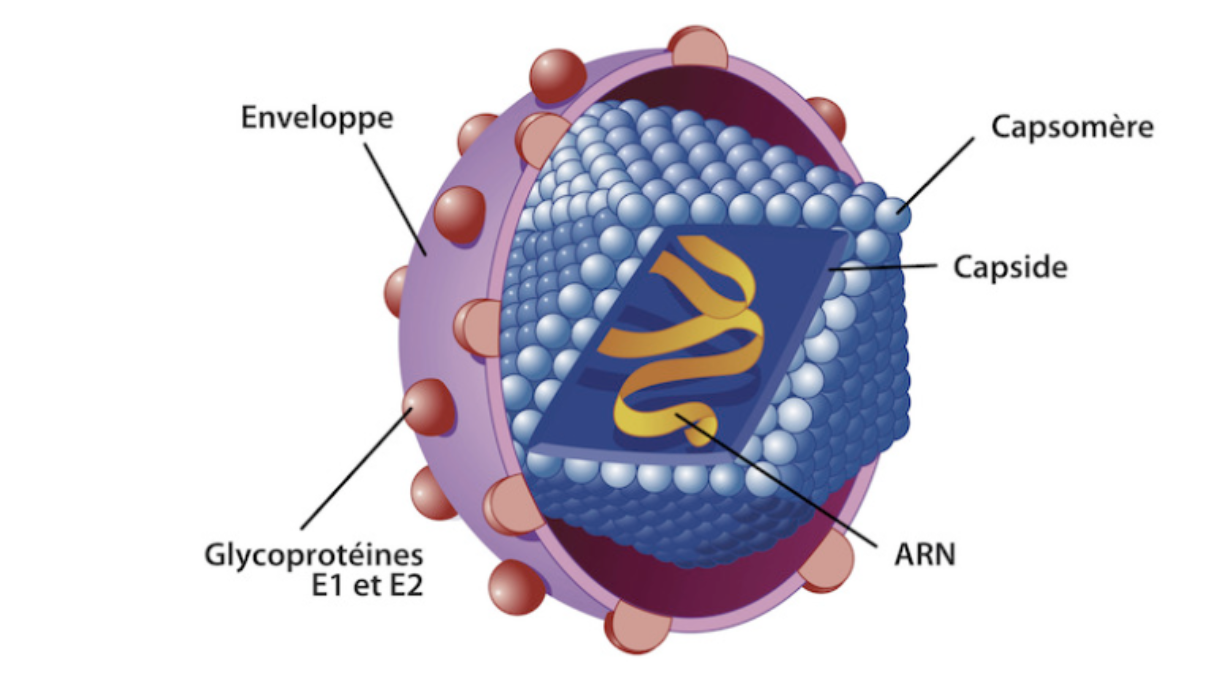
\includegraphics[width=1\textwidth]{./Image/partieVHC.png}
\caption[Différentes parties du VHC] {Différentes parties du VHC: la partie violet répresente l'enveloppe du VHC où à sa surface il y'a les deux glycoprotéines (E1,E2); à l'intérieur de l'envelope, le bleu correspond à la capside c'est une protéine qui protège l'ARN; le jaune est l'ARN virale du VHC;  source: \cite{mennecierVirusLhepatiteMonhepatogastro2022}}
\label{fig:virusVHC}
\end{figure}
 
 \subsubsection {Structure du génome du VHC}
 
 Le génome du VHC est  un ARN monocaténaire linéaire de polarité positive d’environ 9,6 kb. le génome se compose de trois parties: 
 \begin{itemize}
 \item une région 5’ non codante (5’UTR) qui est composée de 341 à 344 nucléotides, est structuré en quatre domaines tige boucle;
 \item le cadre de lecture ouvert (ORF,Open Reading Frame ) est de taille variable (9 024 à 9 111 nucléotides) selon les isolats.  La traduction du ORF code une polyprotéine qui est clivée co- et post-traductionnellement en dix protéines: protéines virales structurales (capside, E1 et E2), de p7 est une protéine qui semble jouer un rôle essentiel dans la morphogenèse du virus et des protéines non structurales (NS1, NS2, NS3, NS4A, NS4B, NS5A et NS5B);
 \item une région 3’ non codante (3’UTR) présente une longueur variable de 200 à 235 nt, elle est constituée (de 5’ en 3’) d’une région non traduite directement en aval de la protéine NS5B \cite{pawlotskyVirusLhepatite2002,VirusLhepatite2025} (figure~\ref{fig:structVHC}).
 \end{itemize}

\begin{figure}[h]
\centering
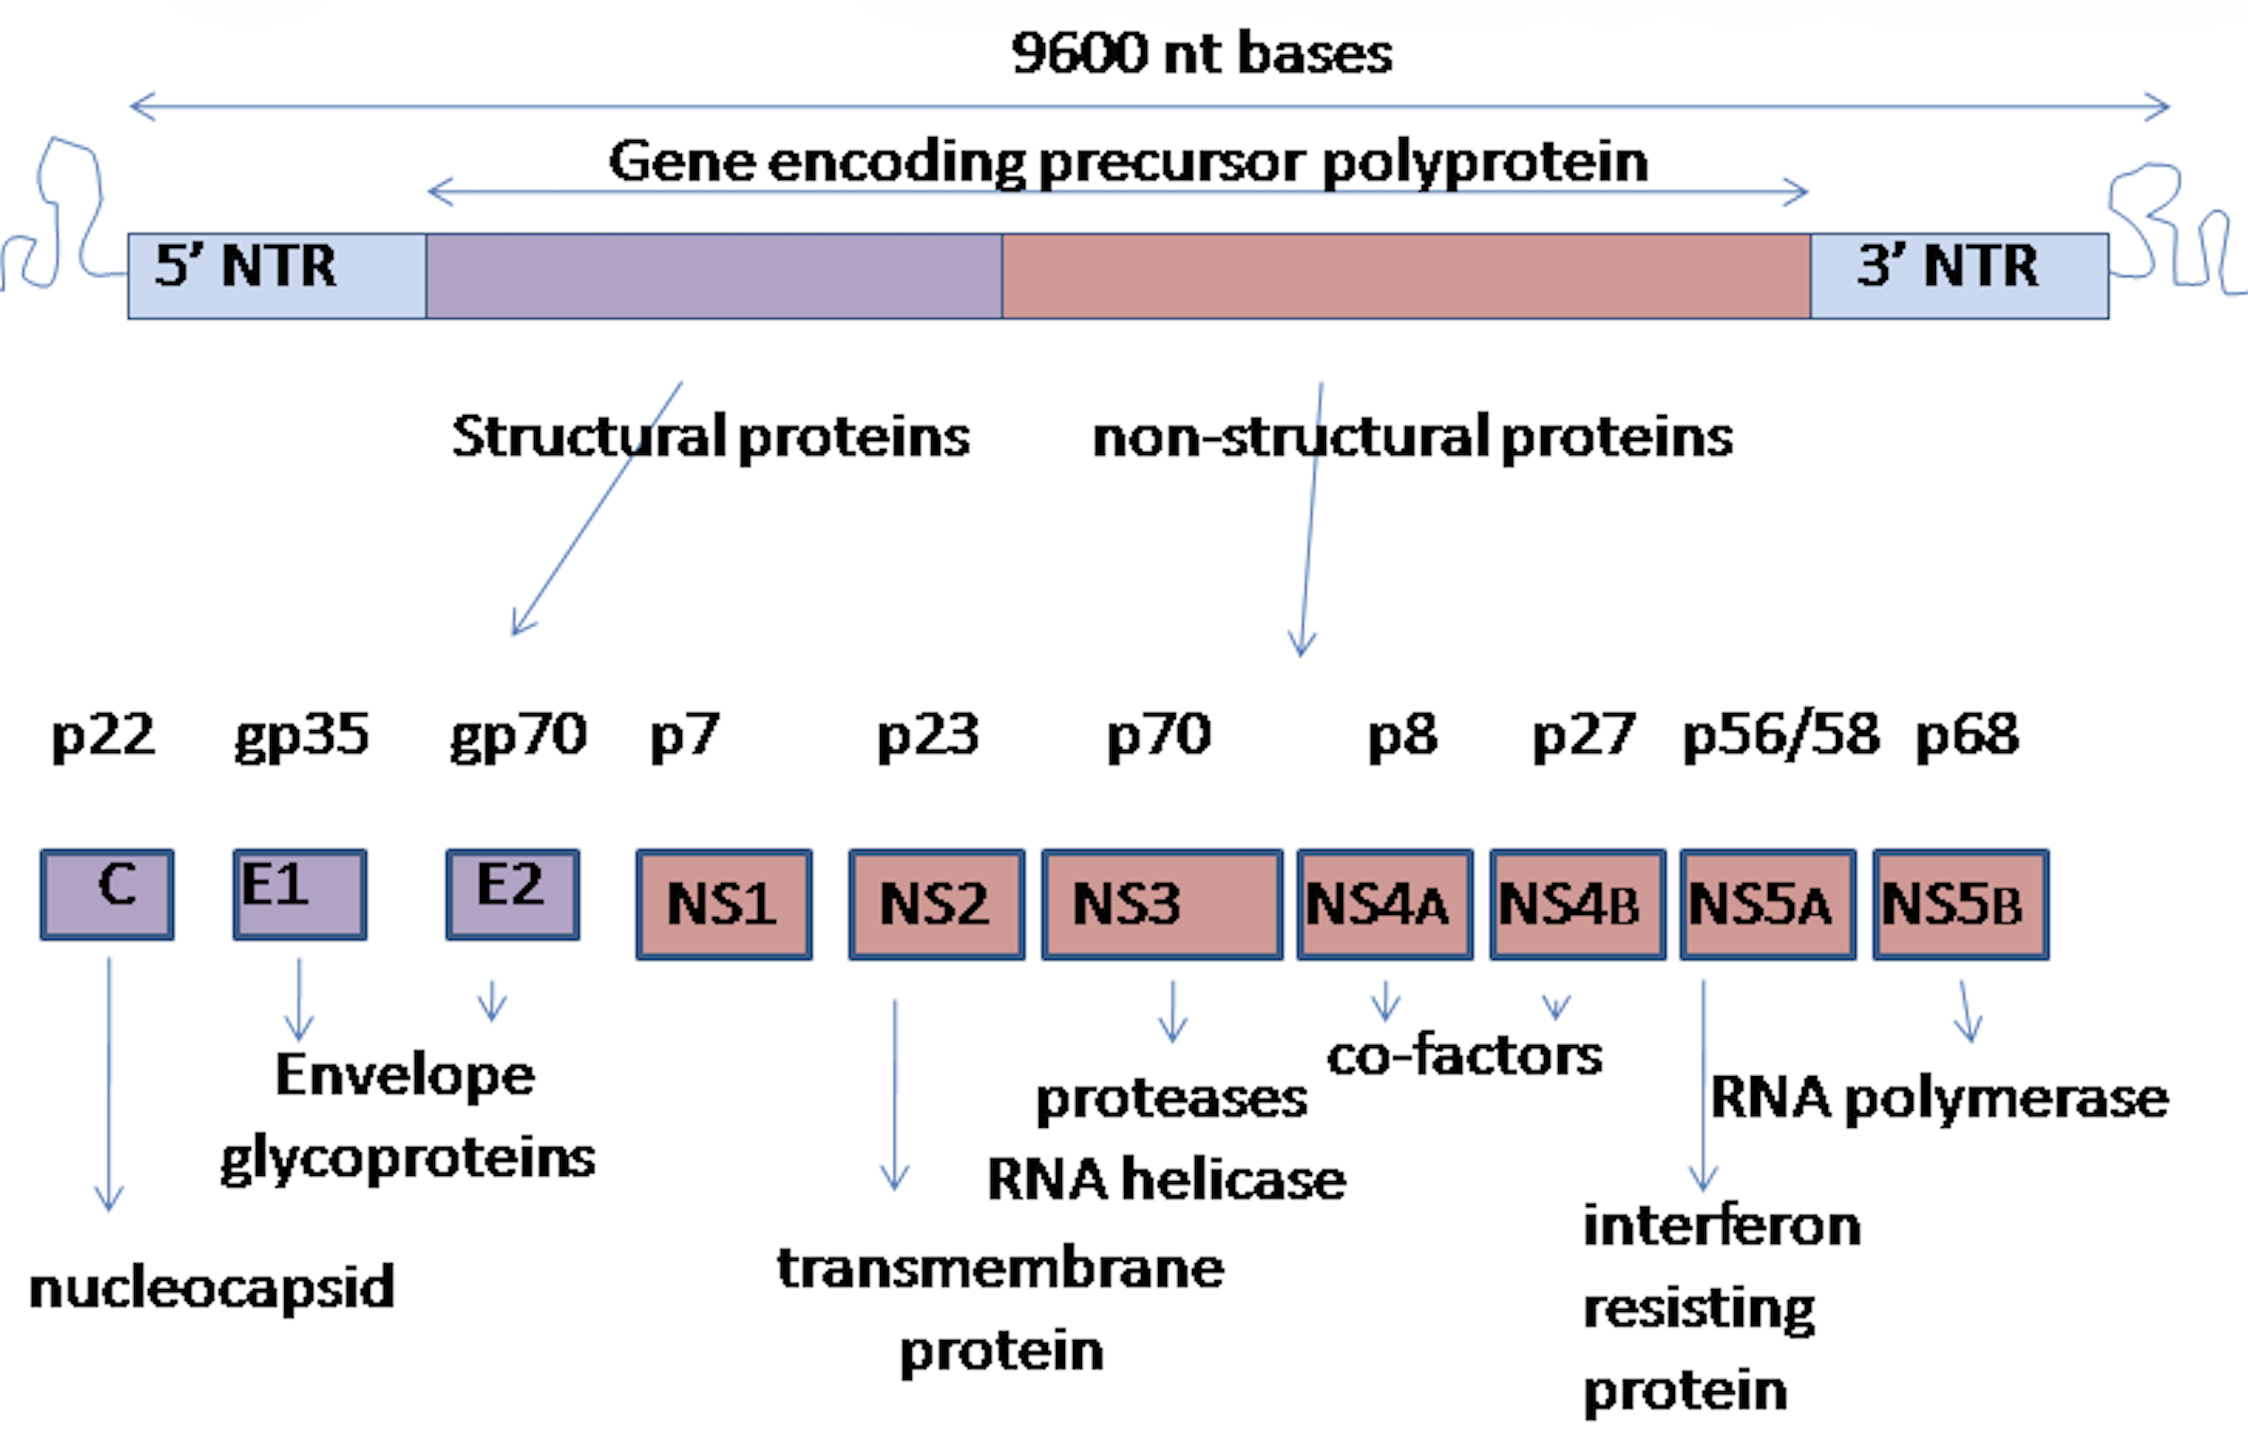
\includegraphics[width=1\textwidth]{./Image/VHC_genome.png}
\caption[Structure du genome VHC] {Structure du genome VHC: la taille du génome est 9,6 kb, les deux extrèmités sont les régions non codantes (5’UTR et 3’UTR), nous avons le ORF qui est composé de deux parties une partie structurale (violet claire) qui traduit des protéines capside (core), E1 et E2 sont très hypervariables et une partie Non structurale (rose claire). nous on s'interesse à la région NS5B qui est une région stable et fiable pour le génotypage; source: \cite{VirusLhepatite2025}}
\label{fig:structVHC}
\end{figure}

 \subsubsection {Génotypes et modes de transmissions du VHC}
 
 Le VHC comprend 7 à 8 génotypes (numérotés de 1 à 7 ou 8) et plus de 100 sous-types, qui diffèrent par leur répartition géographique, leur réponse au traitement et leur impact épidémiologique \cite{chevaliezVirusLhepatiteVHC, FlaviviridaeClassificationLHepacivirus}. Il est présent dans toutes les régions définies par l'OMS. La charge de morbidité la plus élevée se situe dans la région de la Méditerranée orientale, avec 12 millions de personnes infectées chroniquement. L'Asie du Sud-Est et l'Europe environ 9 millions de personnes infectées, la région du Pacifique occidental environ 7 millions, l’Afrique 8 millions et les Amériques 5 millions \cite{Hepatitisb}. Les génotypes 1,2,3 sont largement répandus dans le monde, tandis que les génotypes 5 et 6 sont fréquents en Afrique du Sud et en Asie du Sud-Est. Le génotype 4 est prédominant en Afrique centrale et en Afrique du Nord. Les génotypes 1 et 2 sont plus fréquents en Afrique de l'Ouest \cite{zebaCharacterisationHepatitisVirus2014}.\\
 
 
 Les nouvelles infections surviennent principalement chez les populations à haut risque, telles que les personnes s'injectant des drogues (UDI), les hommes ayant des rapports sexuels avec des hommes (HSH) et les travailleuses du sexe (TS). En Afrique subsaharienne, la transmission se fait essentiellement par des sources iatrogène (une voie de transmission liée aux soins médicaux ou aux pratiques de santé (faux soins, matériel utilisé, transfusions, etc.) . D'autres modes de transmission incluent les piqûres d'aiguilles chez les professionnels de santé, la transmission mère-enfant, les pratiques sexuelles entraînant une exposition au sang, ainsi que certaines pratiques sociales comme le piercing, la scarification, le tatouage etc. \cite{ouobaEpidemiologicProfileHepatitis2021, Hepatitisb}.
 
 
 \subsubsection  {Quasi-espèce (diversité) virale}
  
Comme de nombreux autres virus à ARN, le taux de mutation du VHC est très élevé pouvant aller jusqu’à 10 puissances 12 virions produits par jour.  En conséquence, au sein d’un même patient infecté on peut retrouver un mélange de populations virales étroitement apparenté mais distinctes appelé quasi-espèce. La distribution en quasi-espèces du VHC favorise sa survie. En effet, la présence simultanée de variants viraux différents et la rapidité avec laquelle de nouveaux variants émergent permettent la sélection rapide et continue des variants les mieux adaptés à l’environnement au sein duquel le virus se réplique. La capacité d’adaptation des quasi-espèces virales aux modifications de l’environnement joue un rôle important dans la physiopathologie de l’infection, aussi bien dans les mécanismes de persistance virale que dans la résistance aux traitements antiviraux ou la récidive de l’infection après transplantation hépatique \cite{pawlotskyVirusLhepatite2002,mennecierVirusLhepatiteMonhepatogastro2022}.


\subsection{Ménage}

Au sens statistique, un ménage est l'ensemble des personnes qui vivent habituellement dans un même logement, sans qu'il soit nécessaire qu'elles aient un lien de parenté \cite{MenageInsee}. \\
Selon l'Institut National de la Statistique et de la Démographie (INSD) du Burkina Faso, un ménage ordinaire est l'unité de base utilisée dans les enquêtes statistiques. Il désigne un groupe de personnes apparentées ou non vivant dans le même logement, qui mettent en commun leurs ressources et satisfassent ensemble à leurs besoins essentiels. Le ménage peut être composé d’une seule personne ou de plusieurs personnes, par exemple un chef de ménage (homme), son épouse  ou ses épouses, ses enfants non mariés ou d’autres personnes vivant ensemble \cite{BurkinaFasoRecensement}. Les ménages où l'on observe au moins deux (02) cas d'infection par le VHC sont considérés comme des foyers multiples ou clusteurs du VHC. \\


La transmission intrafamiliale est une transmission qui s'est faite au sein du ménage (foyer). on peut avoir plusieurs transmission intrafamiliale tels que la transmission verticale (du mère à l'enfant), une transmission entre le mari et sa femme mais dans le cadre de cette étude, on va juste regarder la transmission intra sans rentré dans les détaillés.

\newpage 

\section{Contexte de l'étude}

Dans cette section, nous allons parler du lieu de l'étude (cadre), ainsi que de la population d'étude et comment ils ont diagnostiqué les cas VHC, ensuite présenter notre question de recherche. Par ailleurs, la méthode de séquençage utilisé et les études similaires qui ont été méné dans le monde qui a une rélation avec  notre question de recherche.

\subsection{Cadre de l'étude}
L'étude a été méné au Burkina Faso plus précisement dans la région du Sud-Ouest appélé actuellement la région de \textbf{Djôrô}. Cette région est l’une des 17 régions administratives du Burkina Faso. Située dans la partie Sud-Ouest du pays, elle  couvre environ 16 317 Km² et partage des frontières avec le Ghana et la Côte d’Ivoire. Elle comprend 4 provinces: la Bougouriba, le Ioba, le Noumbiel et le Poni et 28 départements. Elle compte 4 communes urbaines, 24 communes rurales et 1084 villages. La population totale estimée en 2024 est de 986 700  habitants avec une densité de 61 hab./km\textsuperscript{2} \cite{Djoro2026} (figure~\ref{fig:carte}).
\newpage
\begin{figure}[h]
\centering
\includegraphics[width=1\textwidth]{./Image/image1.png}
\caption[Région Djôrô] {Situation géographique de la région de Djôrô: en haut à gauche nous avons la carte du Burkina Faso avec ces pays limitrophes où on a le Mali au nord-ouest, le Niger à l'est-nord-est, le Bénin à l'est-sud-est, le Togo au sud-est, le Ghana au sud et la Côte d'Ivoire au sud-ouest. À l'interieur de la carte on a la répartition spatiale des 17 régions administratives et la couleur jaune cible la localisation de la région Djôrô qui a été agrandi au centre de la figure où on a illustré les 4 provinces: la Bougouriba, le Ioba, le Noumbiel et le Poni}
\label{fig:carte}
\end{figure}

\subsection{Type et période de l’étude}
Il s’agissait d’une étude rétrospective utilisant les données issues du projet ANRS REVERSO 1 mené en 2020 dans les ménages de la région de Djôrô Burkina Faso.

\subsection{Population de l'étude \& diagnostic du VHC}

L'étude a été menée auprès des ménages dans la région de Djôrô. Le dépistage de l’hépatite C sur le terrain, a été réalisé à l’aide des tests de diagnostic rapides (TDR) de détection des anticorps anti-VHC. Ce test a été réalisé sur place par les infirmiers (es) de l’équipe d’enquête qui se déplaçaient dans les ménages pour l’étude. Le test a été réalisé suivant les procédures de l’étude en conformité avec les instructions du fabricant (cf. SOP Dépistage VHC par TDR).\\
Chez les sujets dépistés anti-VHC positif par le TDR, un prélèvement de trois à cinq gouttes de sang ont été recueillies sur une carte de papier buvard en raison d’une goutte dans chaque cercle de la carte de type Whatman 903 (Dried Blood Spots (DBS)) a été utilisé. Le prélèvement pour le DBS, s’est fait au bout du doigt pour les adultes et enfants de plus de 2 ans et au talon pour les enfants de moins de 2 ans. Pour la confirmation des cas VHC, un test Cobas AmpliPrep/Cobas TaqMan (qPCR) a été utilisé ce qui permet la détection et la quantification de l'ARN du VHC. L’infection par le VHC a été  confirmée si et seulement si ce test est positif avec ou sans une importante quantité d’ARN viral. En effet, la présence d’ARN VHC signe une infection en cours. Lorsque le test ARN était négatif, il n’y a pas d’infection du VHC. Dans ce cas, il peut s’agir d’un faux positif au TDR anti-VHC ou d’une infection ancienne guérie.

\subsection{Question de recherche de mon stage}

Suite au diagnostic du VHC dans les ménages, nous avons identifié des clusters de ménages comportant au moins deux cas d’infection par le VHC au sein du même ménage. À la suite de ces résultats, nous nous sommes posé la question suivante : \textbf {les cas de VHC sont-ils transmis au sein d’un même ménage dans cette région du Burkina Faso en 2020 ?}

\subsubsection{Objectif général}
Pour répondre à notre question de recherche, nous allons étudier la transmission du VHC au sein des ménages infectés dans la région du Djôrô du Burkina Faso en 2020.

\subsubsection {Objectifs Spécifiques}

Il s’agissait, plus spécifiquement de :
\begin{itemize}
 \item Décrire le flow chart des participants;
 \item Décrire les caractéristiques socio-démographiques des deux groupes (foyers et contrôles) ;
 \item Décrire la diversité virale globale dans les deux groupes à partir des séquences consensus ;
 \item Réaliser une analyse phylogénétique en utilisant la méthode des distances et le maximum de vraisemblance à partir de la séquence primaire.
 \end{itemize}

\subsection{Séquençage: méthode Sanger}

Suite à la confirmation des cas par qPCR, les échantillons provenant des foyers multiples ont été sélectionnés pour le séquençage. Deux régions du génome viral ont été ciblées : la région NS5B (région non structurale) et la région Core, utilisée en cas d’impossibilité d’obtenir la région NS5B. Le séquençage de Sanger a été réalisé sur les échantillons issus des foyers multiples, ainsi que sur un groupe contrôle constitué de ménages ne présentant qu’un seul cas de VHC.\\


Le VHC étant un virus à ARN monocaténaire, le séquençage nécessite une étape préalable de RT-PCR (Reverse Transcription-PCR). Cette étape est essentielle pour les virus à ARN, car elle permet de rétro transcrire l’ARN viral en ADN complémentaire (ADNc) grâce à l’enzyme transcriptase inverse. L’ADNc obtenu a été  ensuite amplifié par PCR afin de produire une quantité suffisante de matériel génétique. Les matériels génétiques amplifiés ont été finalement soumis au séquençage de Sanger pour déterminer les séquences nucléotidiques des régions d’intérêt (NS5B) (figure~\ref{fig:Processus}) qui illustre le processus avant le séquençage.

\begin{figure}[h]
\centering
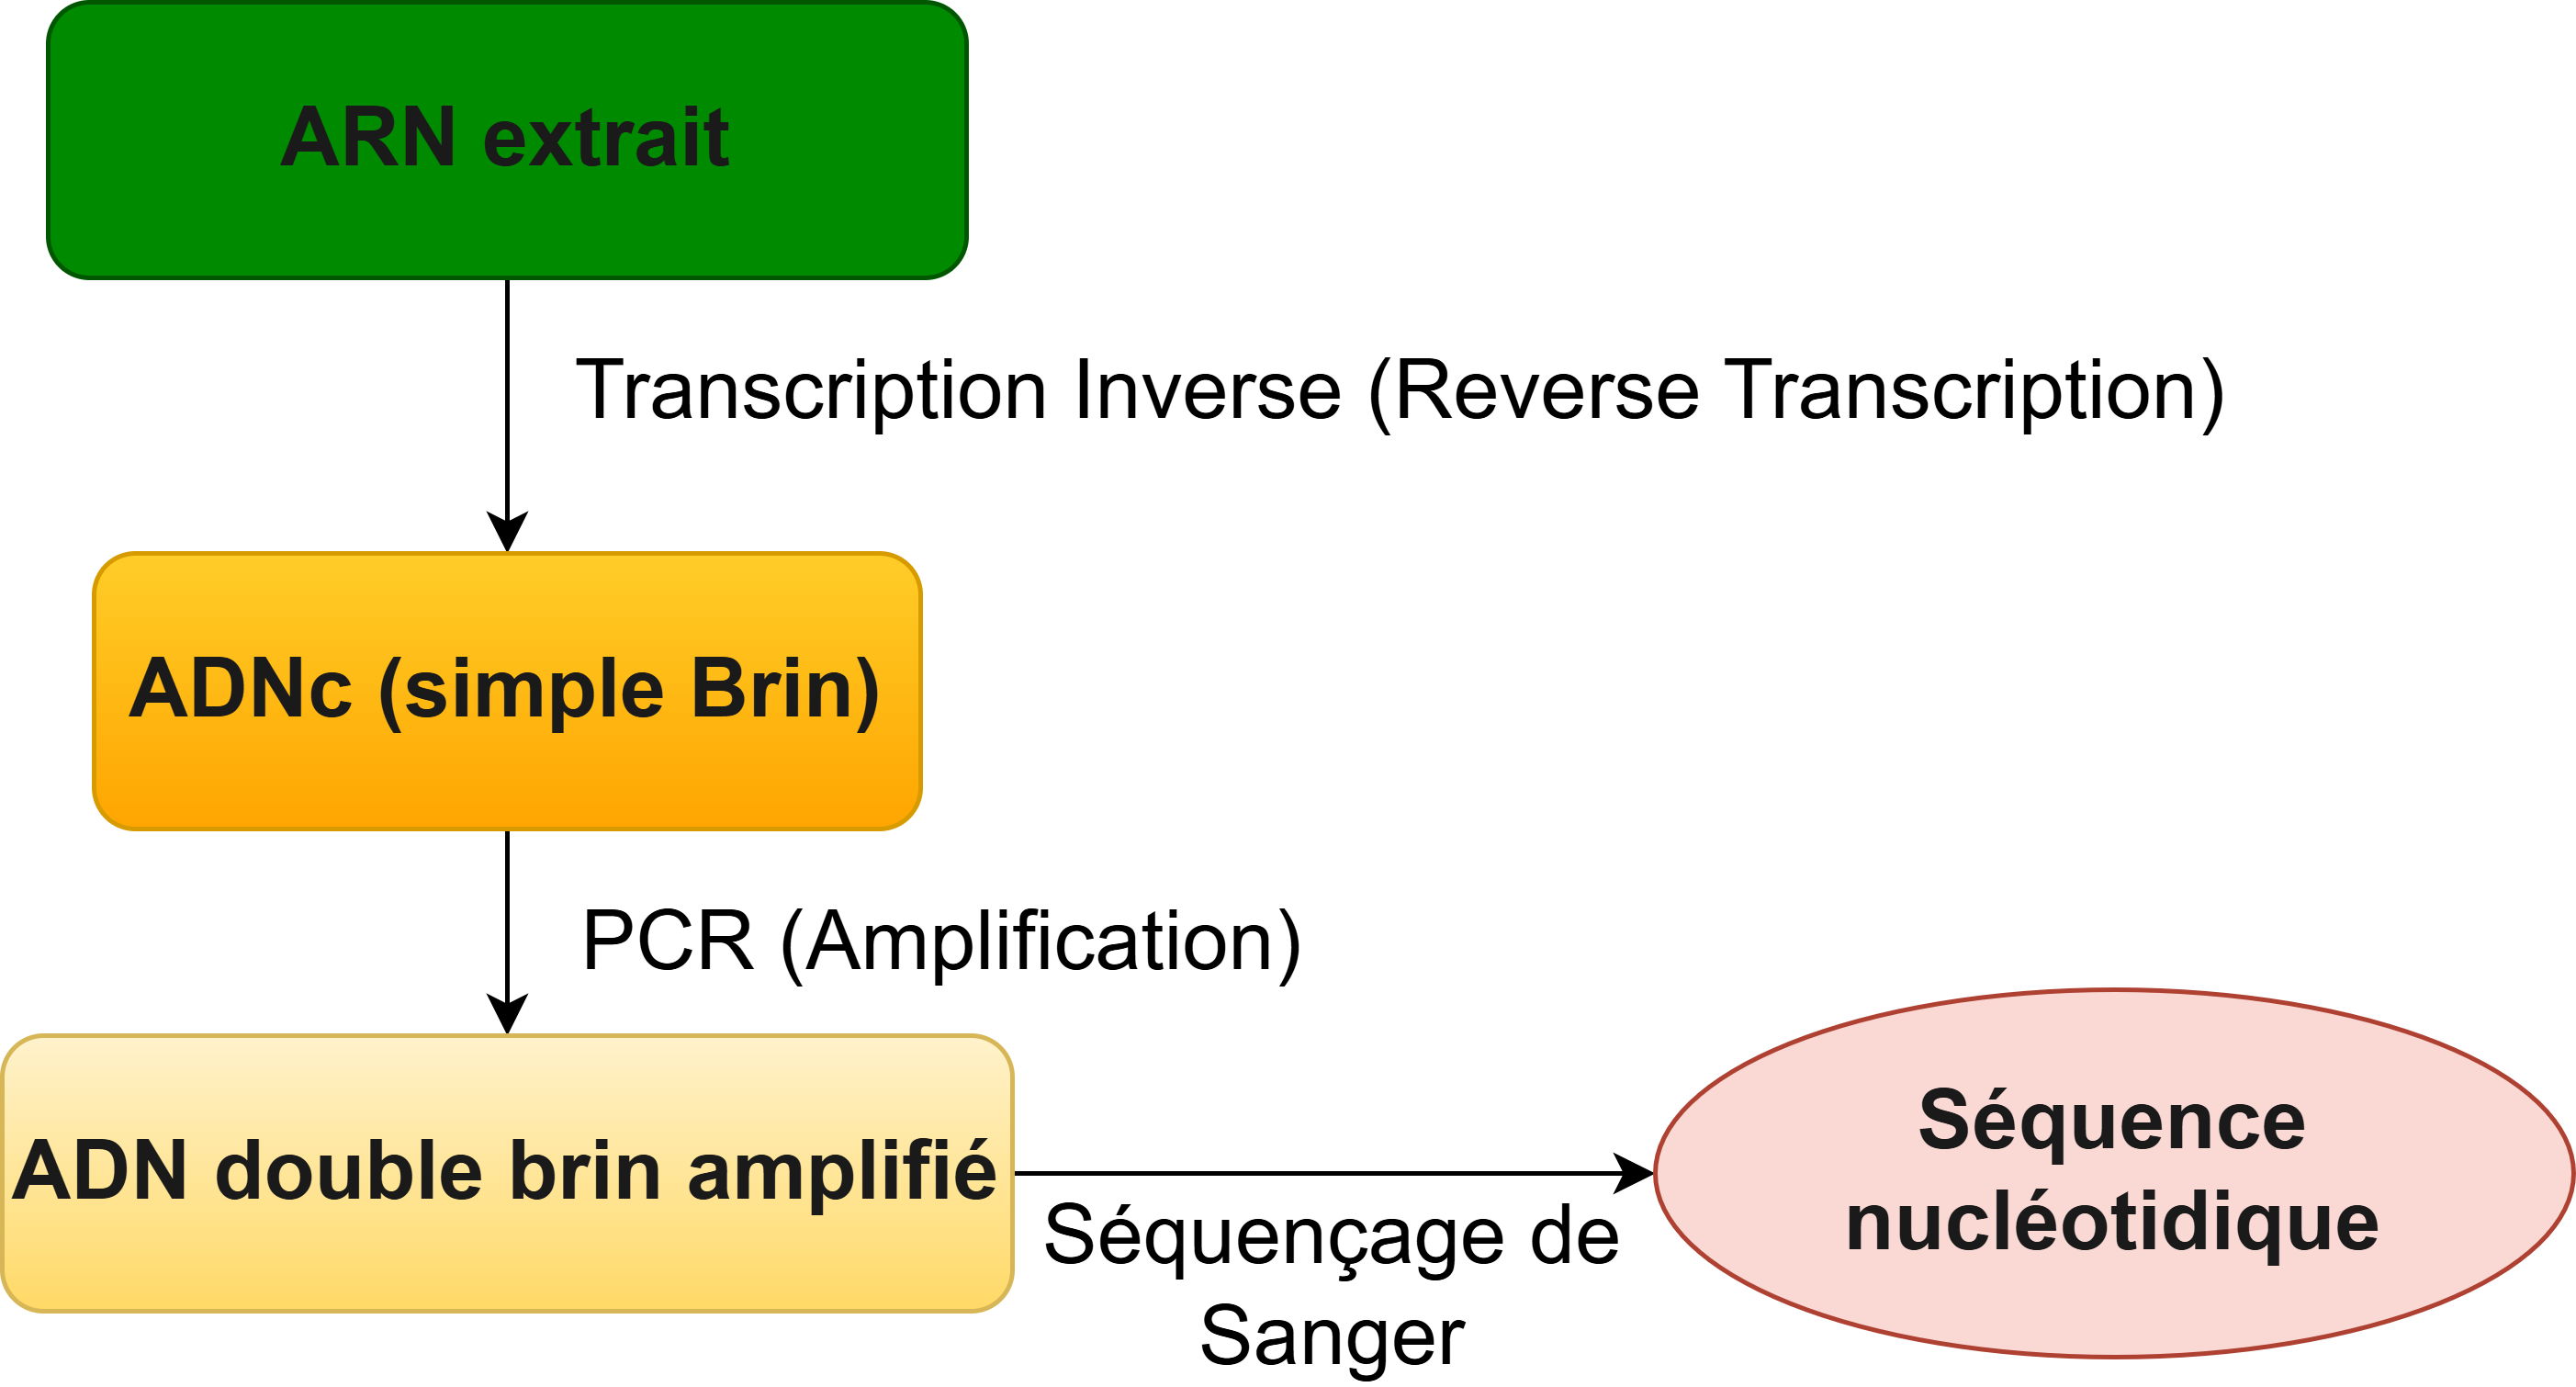
\includegraphics[width=1\textwidth]{./Image/processu.png}
\caption[Processus Sanger] {Processus de la méthode de Sanger: cette figure présente les étapes du séquençage des virus à ARN à partir de DBS (sang séché sur buvard). La couleur verte correspond à l’extraction de l’ARN viral. Après obtention du matériel génétique, une transcription inverse (RT) est réalisée afin de convertir l’ARN en ADN complémentaire ciblant la région d’intérêt. Cette région est ensuite amplifiée par PCR pour produire un ADN double brin. La taille du produit amplifié est contrôlée par électrophorèse sur gel d’agarose, puis l’ADN est soumis au séquençage}
\label{fig:Processus}
\end{figure}

La méthode de Sanger, aussi appelée séquençage par terminaux de chaîne, est une méthode de séquençage d’ADN développée par Frederick Sanger en 1977. Cette méthode nécessite une matrice d’ADN simple brin, une amorce, une ADN polymérase, des désoxynucléotides triphosphates (dNTP) et des didésoxynucléotides triphosphates (ddNTP). Les ddNTP sont des nucléotides dépourvus du groupe 3’OH qui entraîne une modification et stoppent l’élongation de l’ADN. Les ddNTP peuvent être marqués (radioactivité ou fluorescence) pour permettre la détection lors du séquençage. La méthode comprend quatre réactions PCR. Chaque réaction contient les quatre nucléotides normaux, ainsi qu'une solution mère de désoxynucléotides standards (dATP, dGTP, dCTP et dTTP). À chaque réaction, on ajoute un seul des quatre  didésoxynucléotides (ddATP, ddGTP, ddCTP ou ddTTP), les autres nucléotides étant des nucléotides ordinaires. La concentration du désoxynucléotide doit être environ 100 fois supérieure à celle du didésoxynucléotide correspondant (par exemple, 0,5 mM de dTTP : 0,005 mM de ddTTP) afin de produire suffisamment de fragments tout en transcrivant la séquence complète (la concentration de ddNTP dépend également de la longueur de séquence souhaitée). Autrement dit, quatre réactions distinctes sont nécessaires pour tester les quatre ddNTP. Après plusieurs cycles d'extension de l'ADN matrice à partir de l'amorce fixée, les fragments d'ADN obtenus sont dénaturés par la chaleur et séparés par taille par électrophorèse sur gel. À la suite du séquençage, nous obtenons un chromatogramme qui est une représentation graphique du signal électrique produit pendant le séquençage de sanger. Il représente les pics correspondants aux bases (ACGT) \cite{SangerSequencing2026} (figure~\ref{fig:sanger}) 

\begin{figure}[h]
\centering
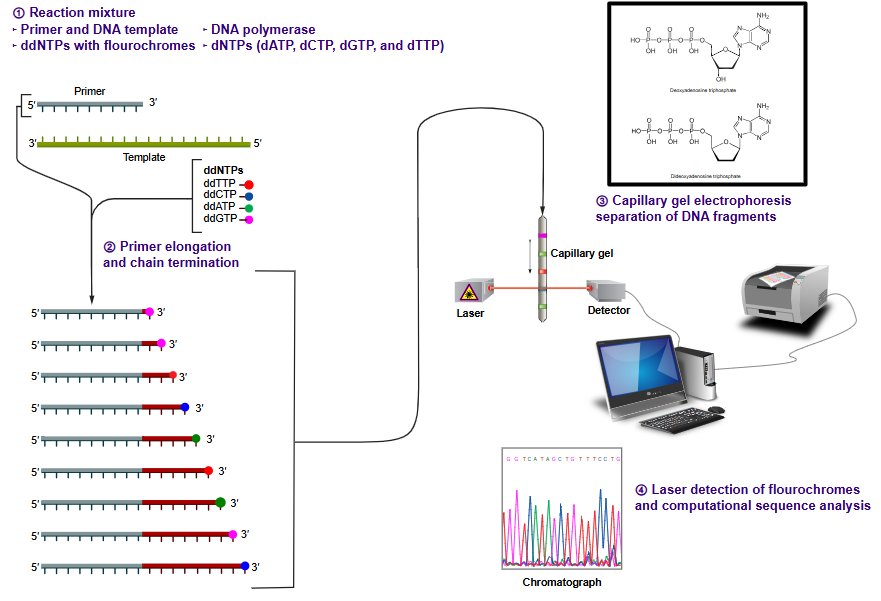
\includegraphics[width=1\textwidth]{./Image/Capture.png}
\caption[Séquençage Sanger] {Séquençage Sanger; souce: \cite{SangerSequencing2026}}
\label{fig:sanger}
\end{figure}

\subsection{Études similaires: révue de la littérature}
Dans cette partie, les articles similaires à notre étude ont été résumé selon leurs méthodologies, les résultats afin de nous appuyer pour pourvoir réaliser notre étude.\\ 


En 2016, \textbf{Vincent Montoya et \textit{al.}} \cite{montoyaDeepSequencingIncreases2016}, ont comparé le séquençage à haut débit au séquençage Sanger pour améliorer la détection des clusters phylogénétiques du VHC. Dans cette analyse, les données viennent de soixante-sept (77) séro convertisseurs du VHC. Un séquençage Sanger a fourni un consensus unique pour chaque individu, et un séquençage à haut débit (illumina) a capturé toutes les variantes intra‑hôte de la région NS5B. Le calcul du seuil pour chaque échantillon utilisé le 50\textsuperscript{e} percentile de la distribution des distances patristiques intra-individu qui sert à identifier les clusters. Les arbres phylogénétiques ont été construits par maximum de vraisemblance en testant sept seuils de distance patristique pour le Sanger: 0,005, 0,01, 0,02, 0,03, 0,04, 0,05, et 0,06. Le seuil de 0,03 a été chosi pour maximiser l’accord positif et négatif avec le deep sequencing. L’analyse comparative compare Sanger et le deep sequencing en examinant les clusters identiques, les nouveaux clusters du deep sequencing et les exclusions du deep sequencing. Sanger et le deep sequencing retrouvent dix (10) individus dans les mêmes clusters. Le deep sequencing ajoute quatre (04) individus à de nouveaux clusters et exclut huit (08) individus que Sanger avait placés dans des clusters, montrant ainsi une meilleure discrimination grâce aux variantes minoritaires. Le seuil Sanger de 0,03 offre le meilleur équilibre d’accord avec le deep sequencing (positif : clusters communs ; négatif : non-clusters).\\
En somme, le deep sequencing surmonte la limite du Sanger (sous-estimation des quasi-espèces) en utilisant un seuil intra-individuel dynamique et en intégrant toutes les variantes pour une phylogénie plus fine. La force de cette étude est que la validation quantitative (accord positif/négatif), application à une cohorte de séro convertisseurs, et démonstration d’un impact concret sur la détection de transmissions. Comme limite de cette étude, une complexité computationnelle du deep sequencing, seuils patristiques à optimiser par dataset, et pas de validation directionnelle des transmissions. Le deep sequencing (illumina) est plus approprié pour obtenir une épidémiologie moléculaire du VHC plus précise, surtout pour les clusters de transmission. \\


 \textbf{Kamila Caraballo Cortes et \textit{al.}(2016)}  \cite{cortesSpousetoSpouseTransmissionEvolution2016}, ont étudié la transmission du VHC entre conjoints et l’évolution des régions HVR1 et 5'UTR par séquençage de nouvelle génération. L’objectif était de déterminer si la souche virale du mari infecté était liée à celle de son épouse atteinte d’une infection chronique depuis 10 ans, tout en suivant l’évolution des variants viraux dans le temps. L’étude portait sur un couple infecté par le sous-type 1b, suivi pendant 9 à 13 mois, ainsi que sur 10 patients chroniques non apparentés utilisés comme contrôles phylogénétiques. Les régions HVR1 et 5'UTR ont été amplifiées par PCR puis séquencées par pyroséquençage 454. La reconstruction des haplotypes a été réalisée avec Shorah, suivie d’un alignement sur les séquences de références 1b et d’une traduction en acides aminés avec MEGA. Les arbres phylogénétiques ont été inférés par maximum de vraisemblance sous le modèle TN93, et l’analyse de l’horloge moléculaire a été réalisée avec MEGA 5.0. La diversité génétique et les paramètres de distance ont été évalués avec DNA SP, la similarité des séquences a été comparée avec la matrice d'identité de Clustal 2.1 et les logos des séquences d'acides aminés ont été générés par Web Logo. \\
 Les résultats révèlent une diversité intra-hôte élevée, avec un nombre important de variants inférés pour HVR1 et 5'UTR, réduits par l’application d’un seuil de fréquence. Au total, 71 923 lectures ont été obtenues. Les résultats ont montré une forte diversité intra-hôte, avec de nombreux variants inférés pour HVR1 et 5'UTR, mais aussi une réduction du nombre de variants après application d’un seuil de fréquence. Une variante minoritaire du donneur, à 1,7\% de fréquence, s’est révélée étroitement apparentée à toutes les variantes du receveur, avec une similitude de 97,1 à 98,3\%. La distance génétique inter-hôtes est restée faible et stable au cours du suivi. L’analyse phylogénétique montre un regroupement des séquences du couple, distinct des contrôles, ce qui soutient l’hypothèse d’une origine virale commune, compatible avec une transmission intra-foyer. \\
Les limites de l’étude incluent un effectif restreint (un seul couple), une fréquence très faible du variant supposé transmis, proche du seuil d’erreur de la méthode, l’impossibilité de conclure avec certitude sur le mode exact de transmission. \\


\textbf {Sofia R. Bartlett, et \textit{al.} } \cite{bartlettPatternsCorrelatesHepatitis2022}, ont publié en 2022 une étude sur l’analyse des patterns de clustering phylogénétique du VHC chez des personnes vivant avec le VIH (PLHIV) dans la cohorte CEASE en Australie, pendant l’ère des antiviraux à action directe (DAA). L’objectif était d’identifier les voies de transmission du VHC chez les PLHIV et d’évaluer des interventions ciblées pour éliminer l’infection. L’extraction d’ARN VHC a été réalisée à partir de gouttes de sang séché (DBS) collectées entre 2014 et 2018 dans la cohorte CEASE (étude prospective sur PLHIV/HCV co-infectés, n=202 avec séquençage). La région Core-E2 du VHC (environ 1,5-2 kb, couvrant des régions hypervariables) a été amplifiée par RT-PCR, puis séquencée par Sanger pour obtenir des séquences de haute-fidélité. Les arbres phylogénétiques ont été construits par Maximum vraisemblance (1000 bootstrap) avec le RAxML, avec un seuil de 3\% de distance génétique pour définir les clusters avec cluster picher et les paires. Une régression logistique mixte a identifié les corrélats du clustering (âge, sexualité, risque sexuel, niveau d’éducation, usage de drogues intraveineuses, etc.). Les résultats montrent que 29\% des 202 séquences (sous-types 1a n=139 ; 3a n=63) appartiennent à des paires ou clusters phylogénétiques. Une forte association est observée chez les personnes de moins de 40 ans (aOR = 2,52 ; IC95\% : 1,20–5,29)  et chez les gays et bisexuels à risque sexuel élevé (aOR = 3,94). Peu de réinfections ont été observées (5 cas), sans lien direct avec les clusters connus. Les clusters sont plus marqués chez les jeunes hommes gays et bisexuels avec un niveau d’éducation supérieur (aOR 2,58). En résumé, la méthodologie Sanger utilisée dans cet article est classique, robuste et adaptée à l’épidémiologie moléculaire pour des régions ciblées comme Core-E2, permettant un clustering fiable sans nécessiter de séquençage haut débit. L’utilisation de DBS (facile à collecter et à stockée), analyse phylogénétique standard (ML + bootstrap élevé), et modélisation statistique pour l’identification des corrélats du clustering. Le Sanger couvre uniquement la région Core-E2 (pas génome entier), le seuil de 3\% est arbitraire, et la directionnalité des transmissions n’est pas établie (inférence indirecte).\\
Cette étude montre la persistance de clusters de transmission sexuelle chez les PLHIV malgré l’ère des DAA, ce qui souligne le besoin d’un traitement rapide et d’une surveillance phylogénétique continue.

\newpage 

\section{Analyses des données}

Ici, nous avons décrit comment on a prétraité les séquences issues du séquençage de sanger, une fois après le prétraitement comment nous avons analysé ces séquences pour répondre à notre question de recherche.

\subsection{Pipeline bioinformatique de prétraitement }

Après le séquençage de Sanger, on obtient des chromatogrammes aux formats .ab1. Ces chromatogrammes  ont été nettoyés en fonction de leur qualité, évaluée à l’aide du score Phred. Ce score correspond à une mesure de la fiabilité de chaque base appelée et reflète la probabilité qu’elle soit incorrecte. le score est definit par:
\[
Q = -10 \log_{10}\left(P_{\mathrm{erreur}}\right)
\]
où où $Q$ est le score Phred et $P_{\mathrm{erreur}}$ est la probabilité qu'une base soit incorrecte. \\
\textbf{Interprétation: }
Plus Q est élevé, plus la base est fiable, car la probabilité d’erreur est faible.\\
\begin {itemize}
\item $Q$=20 correspond à une probabilité d’erreur de 1 sur 100, soit 99\% de fiabilité.
\item  $Q$=30 correspond à une probabilité d’erreur de 1 sur 1000, soit 99,9\% de fiabilité. \\
\end {itemize}
À l’aide du logiciel Chromas, les chromatogrammes ont été visualisés afin de réaliser un contrôle de qualité des pics fluorescents correspondant aux bases nucléiques. En raison du grand nombre d’échantillons, la visualisation manuelle étant longue, un pipeline bioinformatique a été développé en Python (version 3.9.6) en utilisant la bibliothèque Biopython afin d’optimiser et de rendre reproductible le workflow de nettoyage. 
Pour chaque séquence, les régions de faible qualité situées aux extrémités ont été supprimées par trimming, en appliquant un seuil de qualité Phred $Q \ge 20$. Les bases ambiguës (N) résiduelles ont été corrigées en consultant les signaux bruts du chromatogramme aux positions des pics réels.  La séquence primaire a été définie comme la base au signal fluorescent le plus élevé à chaque site (position) et la séquence secondaire comme la deuxième comme le deuxième signal le plus fort avec un seuil de détection de 25\% du signal primaire. Une séquence consensus a été généré en combinant les séquence primaire et secondaire selon la nomenclature du code IUPAC, permettant de capturer les positions présentant une population virale hétérogène détectable (diversité des quasi-espèce). Après le nettoyage, les séquences primaires ont été concaténées entre elles, de même que les séquences secondaires et consensus, à l’aide de la commande « cat », générant ainsi trois fichiers multi-FASTA distincts destinés à l’alignement multiple et aux analyses phylogénétiques (figure~\ref{fig:pipeline}).

\newpage
\begin{figure}[h]
\centering
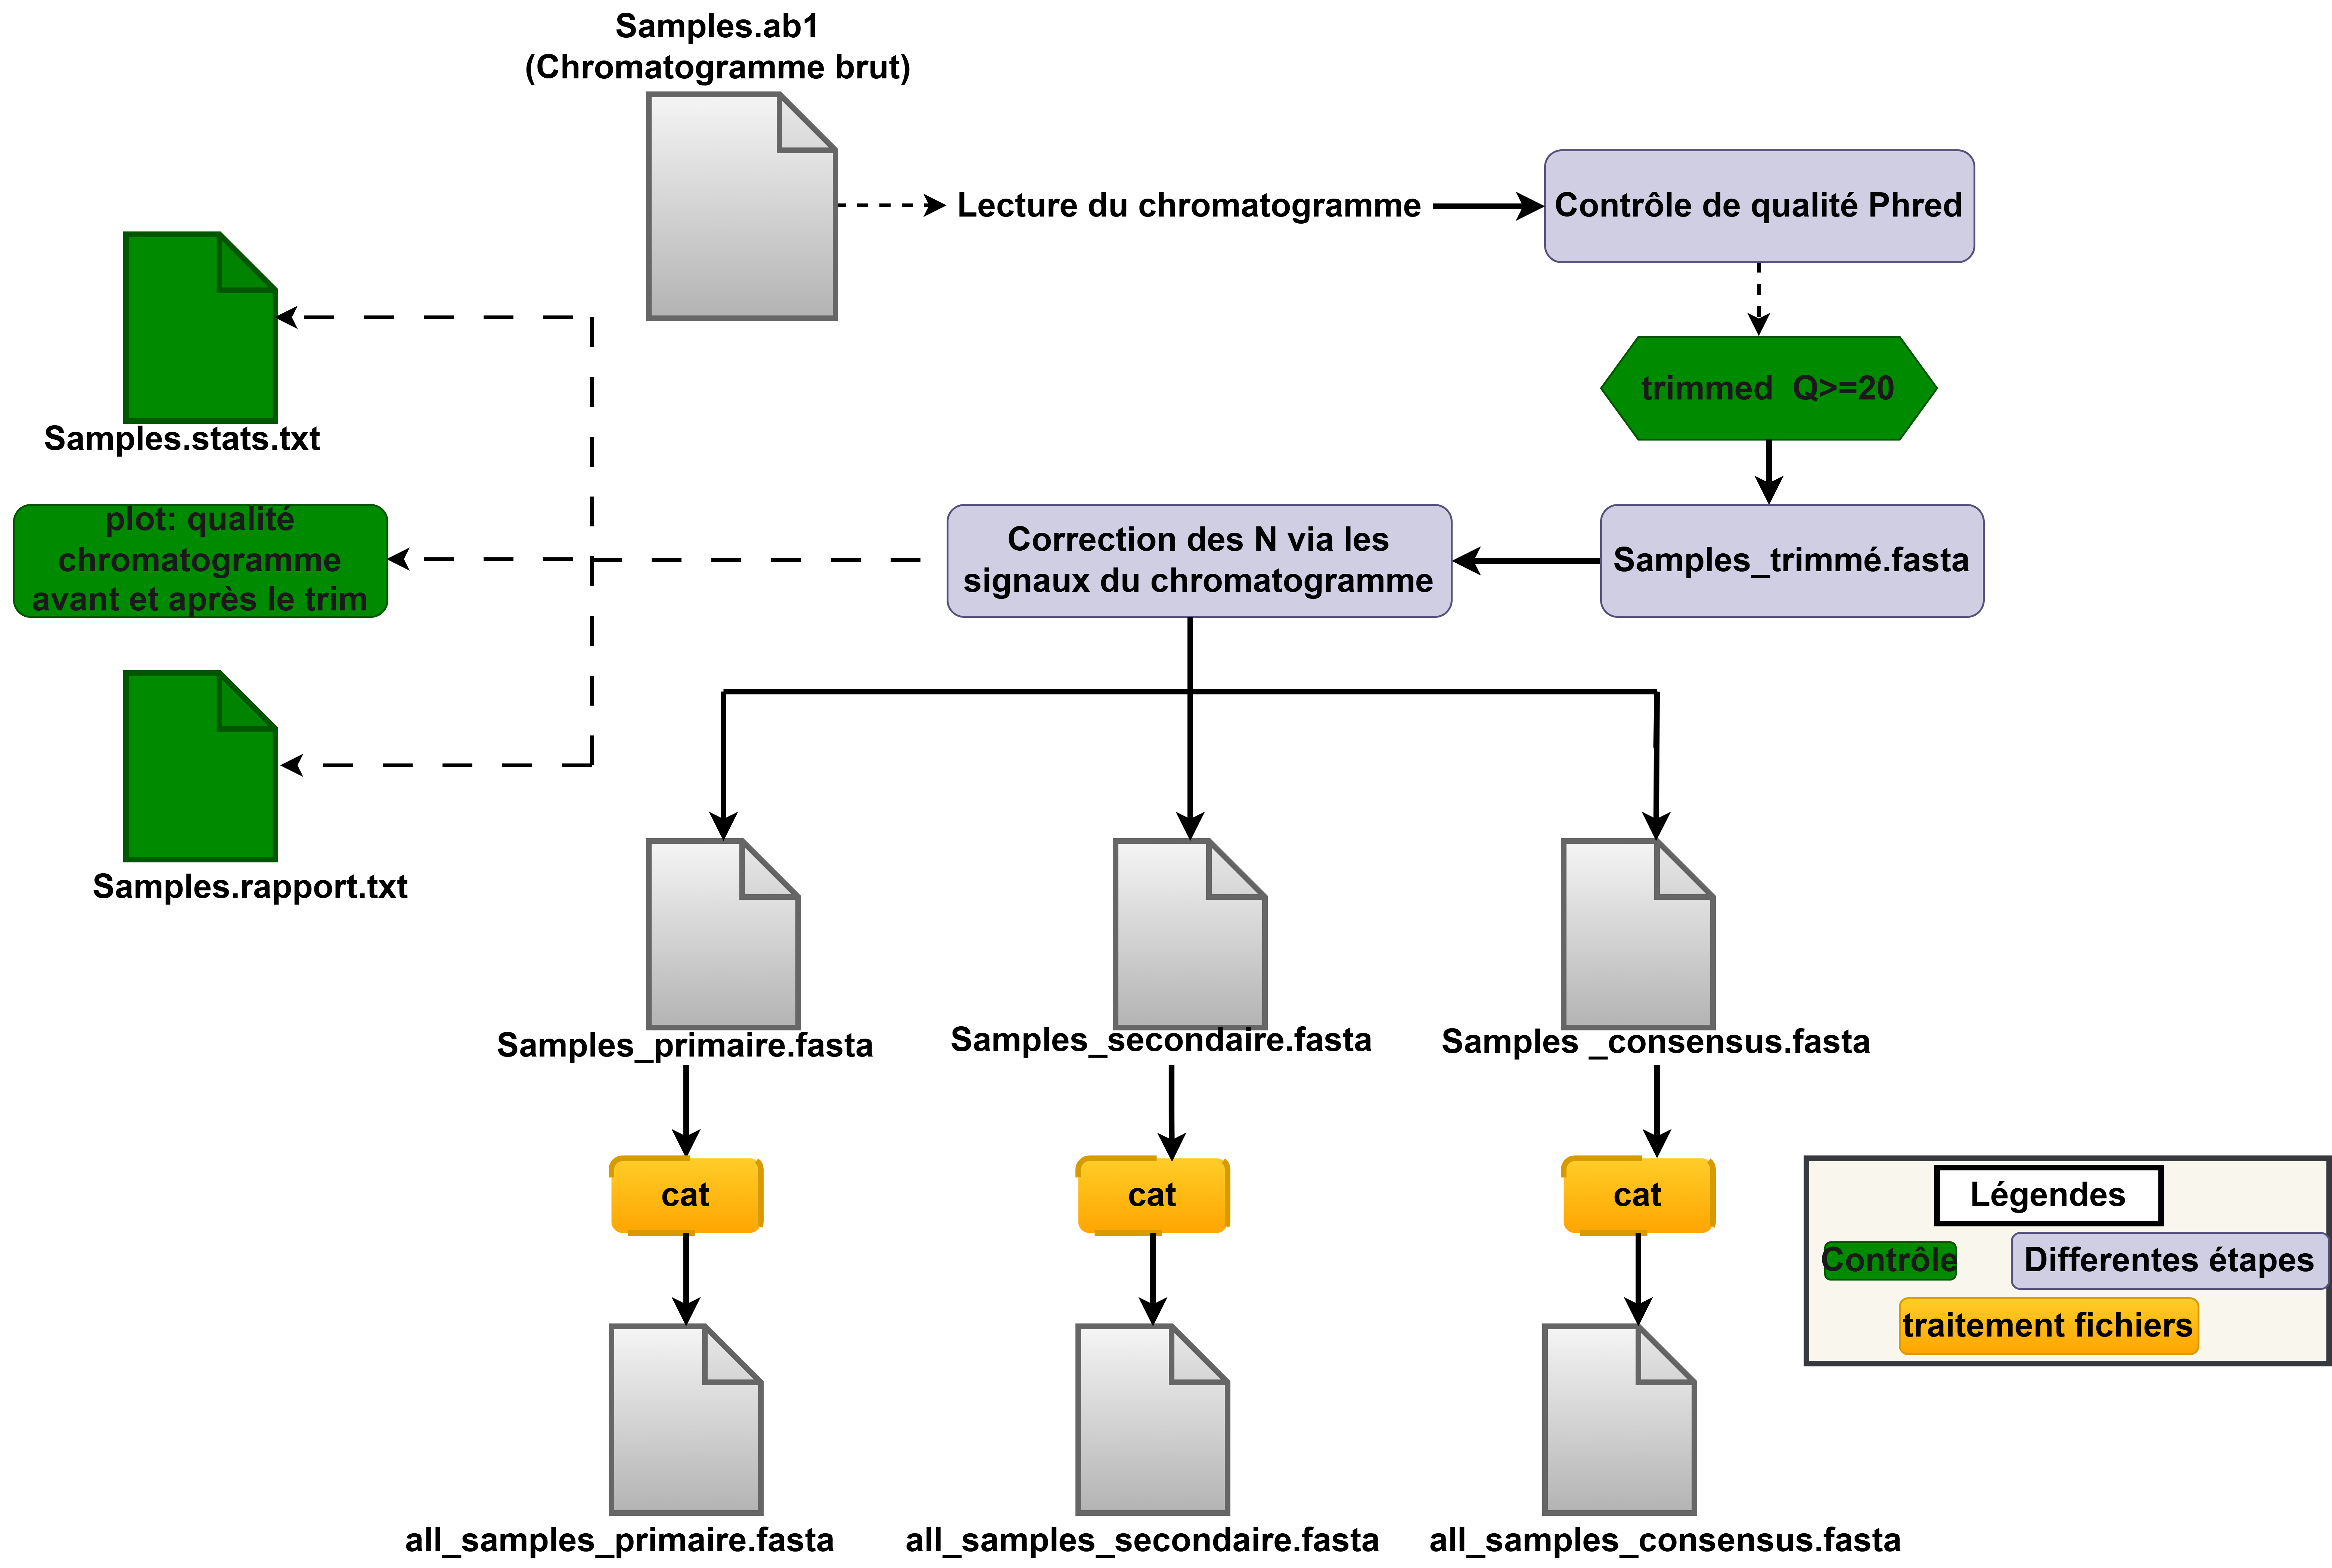
\includegraphics[width=1\textwidth]{./Image/pipeline.png}
\caption[Pipeline de traitement des séquences] {Pipeline de prétraitement des données issues du séquençage de Sanger: notre pipeline prend en entrée les chromatogrammes bruts, qui sont d'abord lus et soumis à un contrôle de qualité. Si la qualité initiale est  mauvaise ($Q < 20$), le programme s'arrêt avec un méssage d'erreur de qualité. Sinon,il poursuit avec le prétraitement, consistant à trimmer les deux extremités à $Q \ge 20$ afin d’obtenir une séquence trimée. \\
Ensuite, les nucléotides N sont corrigés à partir des signaux du chromatogramme. Pour chaque position contenant un N, le programme identifie le pic de signal le plus élevé et remplace le N par le nucléotide correspondant, ce qui génère une séquence primaire. Un deuxième pic, lorsque son signal est supérieur ou égal à 0,25, est également pris en compte pour construire une séquence secondaire. Les deux séquences sont ensuite fusionnées pour produire une séquence consensus, avec correction des positions ambiguës selon le code IUPAC. Des fichiers texte récapitulatifs ainsi que des figures des chromatogrammes avant et après prétraitement ont aussi été générés}
\label{fig:pipeline}
\end{figure}

\subsection [Hétérogénéité génétique intra-hôte du VHC ] {Hétérogénéité génétique intra-hôte (Diversité virale) du VHC dans la population d’étude}

Afin d’étudier l’hétérogénéité génétique intra-hôte au sein de la population d’étude, les séquences consensus des deux groupes (foyers et contrôles) ont été utilisées pour déterminer le nombre de sites nucléotidiques ambiguës dans chaque séquence. Ce paramètre a été considéré comme un indicateur indirect de l’hétérogénéité génétique intra-hôte des populations virales. Le ratio de diversité virale a été calculé à l’aide de la formule ci-dessous:
\[
\text{Ratio} =
\frac{\text{Nombre de sites ambigus}}
{\text{Longueur de la séquence correspondante}}
\times 100
\]

La médiane et l’intervalle interquartile (IIQ) ont été utilisés pour décrire la variation de ce ratio au sein du groupe, suivis d’une analyse de l’hétérogénéité génétique intra-hôte chez les individus appartenant à un même ménage. La comparaison de la diversité virale entre les deux groupes a été réalisée à l’aide du test de Mann-Whitney (test de Wilcoxon).
Pour les séquences consensus issues des foyers, nous avons formulé des hypothèses concernant les événements de transmission du VHC. Nous avons supposé que, pour un individu infecté au sein d’un ménage, la transmission pouvait avoir eu lieu soit à l’intérieur du ménage, soit à l’extérieur. En nous basant sur les distances génétiques, un ménage composé de deux personnes infectées a été considéré comme correspondant à un événement de transmission, tandis qu’un ménage de trois personnes correspondait à trois événements de transmission. Ces événements de transmission ont ensuite été représentés graphiquement.
Afin de déterminer si l’infection était survenue en intra- ou en inter-ménage, un seuil de distance génétique globale a été défini sur la base de la médiane des distances génétiques du groupe contrôle, ainsi que des quantiles à 5\% et 75\%, utilisés comme intervalles de référence. Un seuil de distance génétique de 3\%, basé sur la littérature, a été retenu pour identifier les transmissions probables intra-ménage. Ainsi, les événements de transmission présentant une distance génétique inférieure à 3\% ont été considérés comme des transmissions intra-ménage probables ; ceux situés entre 3\% et 5\textsuperscript{e} percentile comme des transmissions de proximité génétique faible à modérée, ceux compris entre le 5\textsuperscript{e} percentile et la médiane comme des divergences modérées; et ceux supérieur au 75\textsuperscript{e} percentile ont été considérés comme des transmissions inter-ménage.
  

\subsection{Analyses phylogénétiques}
\subsubsection *{Alignement multiple}

L’alignement multiple a été réalisé avec MAFFT (version 7.526) qui est un algorithme de consistance et raffinement itératif. la ligne de commande bash ci-dessous a été utilisée pour lancer l'alignement multiple:
\begin{terminal}
# Commande Bash 
 mafft --auto --reorder sequence_FC_BON.fasta > aligned_sequence_FC_BON.fasta
\end{terminal}
avec deux options importantes (--auto --reorder):  --auto choisit automatiquement la meilleure stratégie d’alignement selon le nombre et le type de séquences, et --reorder réorganise l’ordre des séquences en sortie selon leur similarité. 

\subsubsection * {Distance génétique du VHC}
Pour estimer la distance génétique au sein des foyers, nous avons utilisé la méthode du Neighbor-Joining (NJ), une méthode de clustering ascendant pour la reconstruction d’arbres phylogénétiques, développée par Saitou et Nei en 1987. Cet algorithme repose sur la connaissance des distances génétiques entre chaque paire de séquences  afin de construire l’arbre phylogénétique  \cite{NeighborJoining2026}.\\
En complément de la méthode NJ, nous avons utilisé le modèle de substitution de Tamura-Nei (1993, TN93), qui prend en compte les différences entre les taux de transitions et de transversions, ainsi que les fréquences inégales des bases nucléotidiques (A, C, G, T) et les longueurs de branches. Ce modèle comporte plusieurs paramètres : les fréquences de bases (3 paramètres indépendants), les taux de substitution (2 paramètres), ainsi que les longueurs de branches, soit 2$N - 3$ paramètres pour un arbre non raciné. Au total, le modèle comprend $2N + 2$ paramètres, où N correspond au nombre de séquences (ou feuilles terminales).\\
La matrice de distances génétiques par paires a été calculée sous R (version 4.6.0) à l’aide de la fonction dist.dna(), en utilisant le modèle TN93 avec suppression des positions comportant des gaps par paire (pairwise.deletion = TRUE). Les distances ont été calculées pour toutes les paires de séquences, soit $\frac{n(n-1)}{2}$ comparaisons, puis classées en deux catégories : les distances intra-ménage (entre individus d’un même foyer) et les distances inter-ménage (entre individus de foyers différents).

\subsubsection * {Phylogénétique par Maximum de vraisemblance}
La sélection du meilleur modèle de substitution nucléotidique a été effectuée sous R à l’aide de la fonction modelTest() du package phangorn (version 2.12.1), en comparant les modèles JC69, HKY85, TN93 et GTR, avec et sans distribution gamma (+G) et proportion de sites invariants (+I), selon le critère d’information d’Akaike (AIC). Le modèle présentant la plus faible valeur d’AIC a été retenu.
L’arbre phylogénétique a ensuite été reconstruit par maximum de vraisemblance (ML) avec RAxML, installé via Conda dans un environnement dédié à la phylogénétique, puis exécuté en ligne de commande. Le modèle utilisé dans RAxML a été choisi de manière compatible avec le logiciel. Ainsi, si le modèle retenu par R était différent des modèles directement disponibles dans RAxML, nous avons utilisé le modèle GTR+G (GTRGAMMA) ou GTR+G+I (GTRGAMMAI) \cite{stamatakisRAxMLVersion82014}, qui correspond à l’approximation compatible avec le modèle sélectionné par phangorn. La robustesse topologique de l’arbre a été évaluée par 1 000 réplicats de bootstrap. la ligne de commande est : 

\begin{terminal}
# Activation de l'environnement phylogenetique
conda activate phylogenetics

# Lancement de RAxML
raxmlHPC \
-s alignedFC.fasta \
-n VHCFC \
-m GTRGAMMAI \
-p 12345 \
-x 12345 \
-# 1000 \
-f a
\end{terminal}


\begin{table}[!htbp]
\centering
\caption{Paramètres utilisés pour l'exécution de RAxML}
\label{tab:raxml_parametres}
\begin{tabular}{p{3cm} p{3cm} p{8cm}}
\toprule
\textbf{Paramètre} & \textbf{Valeur} & \textbf{Explication} \\
\midrule
raxmlHPC & -- & Exécutable RAxML pour HPC (High Performance Computing). \\

\texttt{-s} & \texttt{alignedFC.fasta} &
Nom du fichier d'entrée contenant les séquences alignées (format FASTA ou PHYLIP). \\

\texttt{-n} & \texttt{VHCFC} &
Suffixe du nom de sortie ; tous les fichiers générés porteront ce suffixe. \\

\texttt{-m} & \texttt{GTRGAMMAI} &
Modèle de substitution utilisé : GTR + modèle GAMMA d'hétérogénéité des taux + proportion de sites invariants (I). \\

\texttt{-p} & \texttt{12345} &
Graine (\textit{seed}) aléatoire utilisée pour générer l'arbre initial de la recherche par maximum de vraisemblance (ML). \\

\texttt{-x} & \texttt{12345} &
Graine aléatoire utilisée pour le bootstrap rapide (\textit{rapid bootstrap}). \\

\texttt{-\#} & \texttt{1000} &
Nombre de réplicats de bootstrap rapide réalisés. \\

\texttt{-f} & \texttt{a} &
Mode d'exécution : bootstrap rapide suivi de la recherche de l'arbre de maximum de vraisemblance (ML) optimal en une seule exécution. Génère un arbre ML annoté avec les valeurs de bootstrap. \\
\bottomrule
\end{tabular}
\end{table}

un fichier \texttt{RAxML\_bipartitions.VHCFC} a été obtenu qui contient l’arbre ML optimal avec les valeurs de bootstrap annotées sur les nœuds qui a été importé sur R pour la visualisation de l’arbre ML.
Les valeurs de bootstrap supérieures ou égales à 70\,\% ont été considérées comme un support statistique satisfaisant des nœuds internes.


\newpage


\subsection {Analyses statistiques}

Nous avons décrits, les données socio-démographique (age, le sexe, la rélation avec le chef de menage, etc.), des deux groupes (contrôle et foyer). L'âge a été décrit avec la médiane et l’intervalle interquartile (IIQ). La significativité de la différence entre la distance intra et inter-familial à été testée par le test de Mann-Whitney (test de Wilcoxon) ou notre hypothèse alternative: distances intra < distances inter. \\
Afin de représenter la matrice des distances génétiques entre les séquences virales des foyers multiples, une carte de chaleur (heatmap) a été utilisé pour visualiser les distances génétiques entre chaque paire de séquences. Dans cette représentation, chaque case correspond à la distance entre deux individus. Les couleurs claires reflètent une faible distance génétique, alors que les couleurs foncées indiquent une distance génétique plus élevée. La diagonale correspond à la comparaison d'un individu avec lui même donc la distance est nulle. 


\newpage 
\section{Résultats  \& discussions }

\subsection{Diagramme de flux des participants}

Pour cette étude, au total 510 ménages ont été enquêtés, dont 179 comportaient au moins un cas de VHC positif. Parmi ces derniers, 85 ménages présentaient au moins deux cas de VHC au sein du même foyer et ont été considérés comme des foyers multiples. Dans ces foyers multiples, 30 participants ont été sélectionnés pour le séquençage Sanger. Deux régions virales  ont été ciblées, Core et NS5B, mais seule la région NS5B a été retenue pour l’analyse, car elle est décrite dans la littérature comme une région stable et fiable pour le génotypage du VHC. Sur les 30 échantillons, 25 ont été amplifiés avec succès pour la région NS5B. Parmi eux, 18 étaient de génotype 2, génotype particulièrement pertinent dans le contexte de cette étude puisqu’il est le plus répandu en Afrique de l’Ouest selon la littérature. Ces 18 séquences provenaient de 8 ménages appartenant à des foyers multiple (figure~\ref{fig:foyer}). \\
Quant au groupe contrôle, le même filtre a été appliqué. Au total, 80 échantillons ont été sélectionnés, dont 51 amplifiés pour la région NS5B. Parmi ces 51 échantillons, 47 appartenaient au génotype 2 (figure~\ref{fig:controle}). 


\begin{figure}[ht]
    \centering

    \begin{subfigure}{0.48\textwidth}
        \centering
        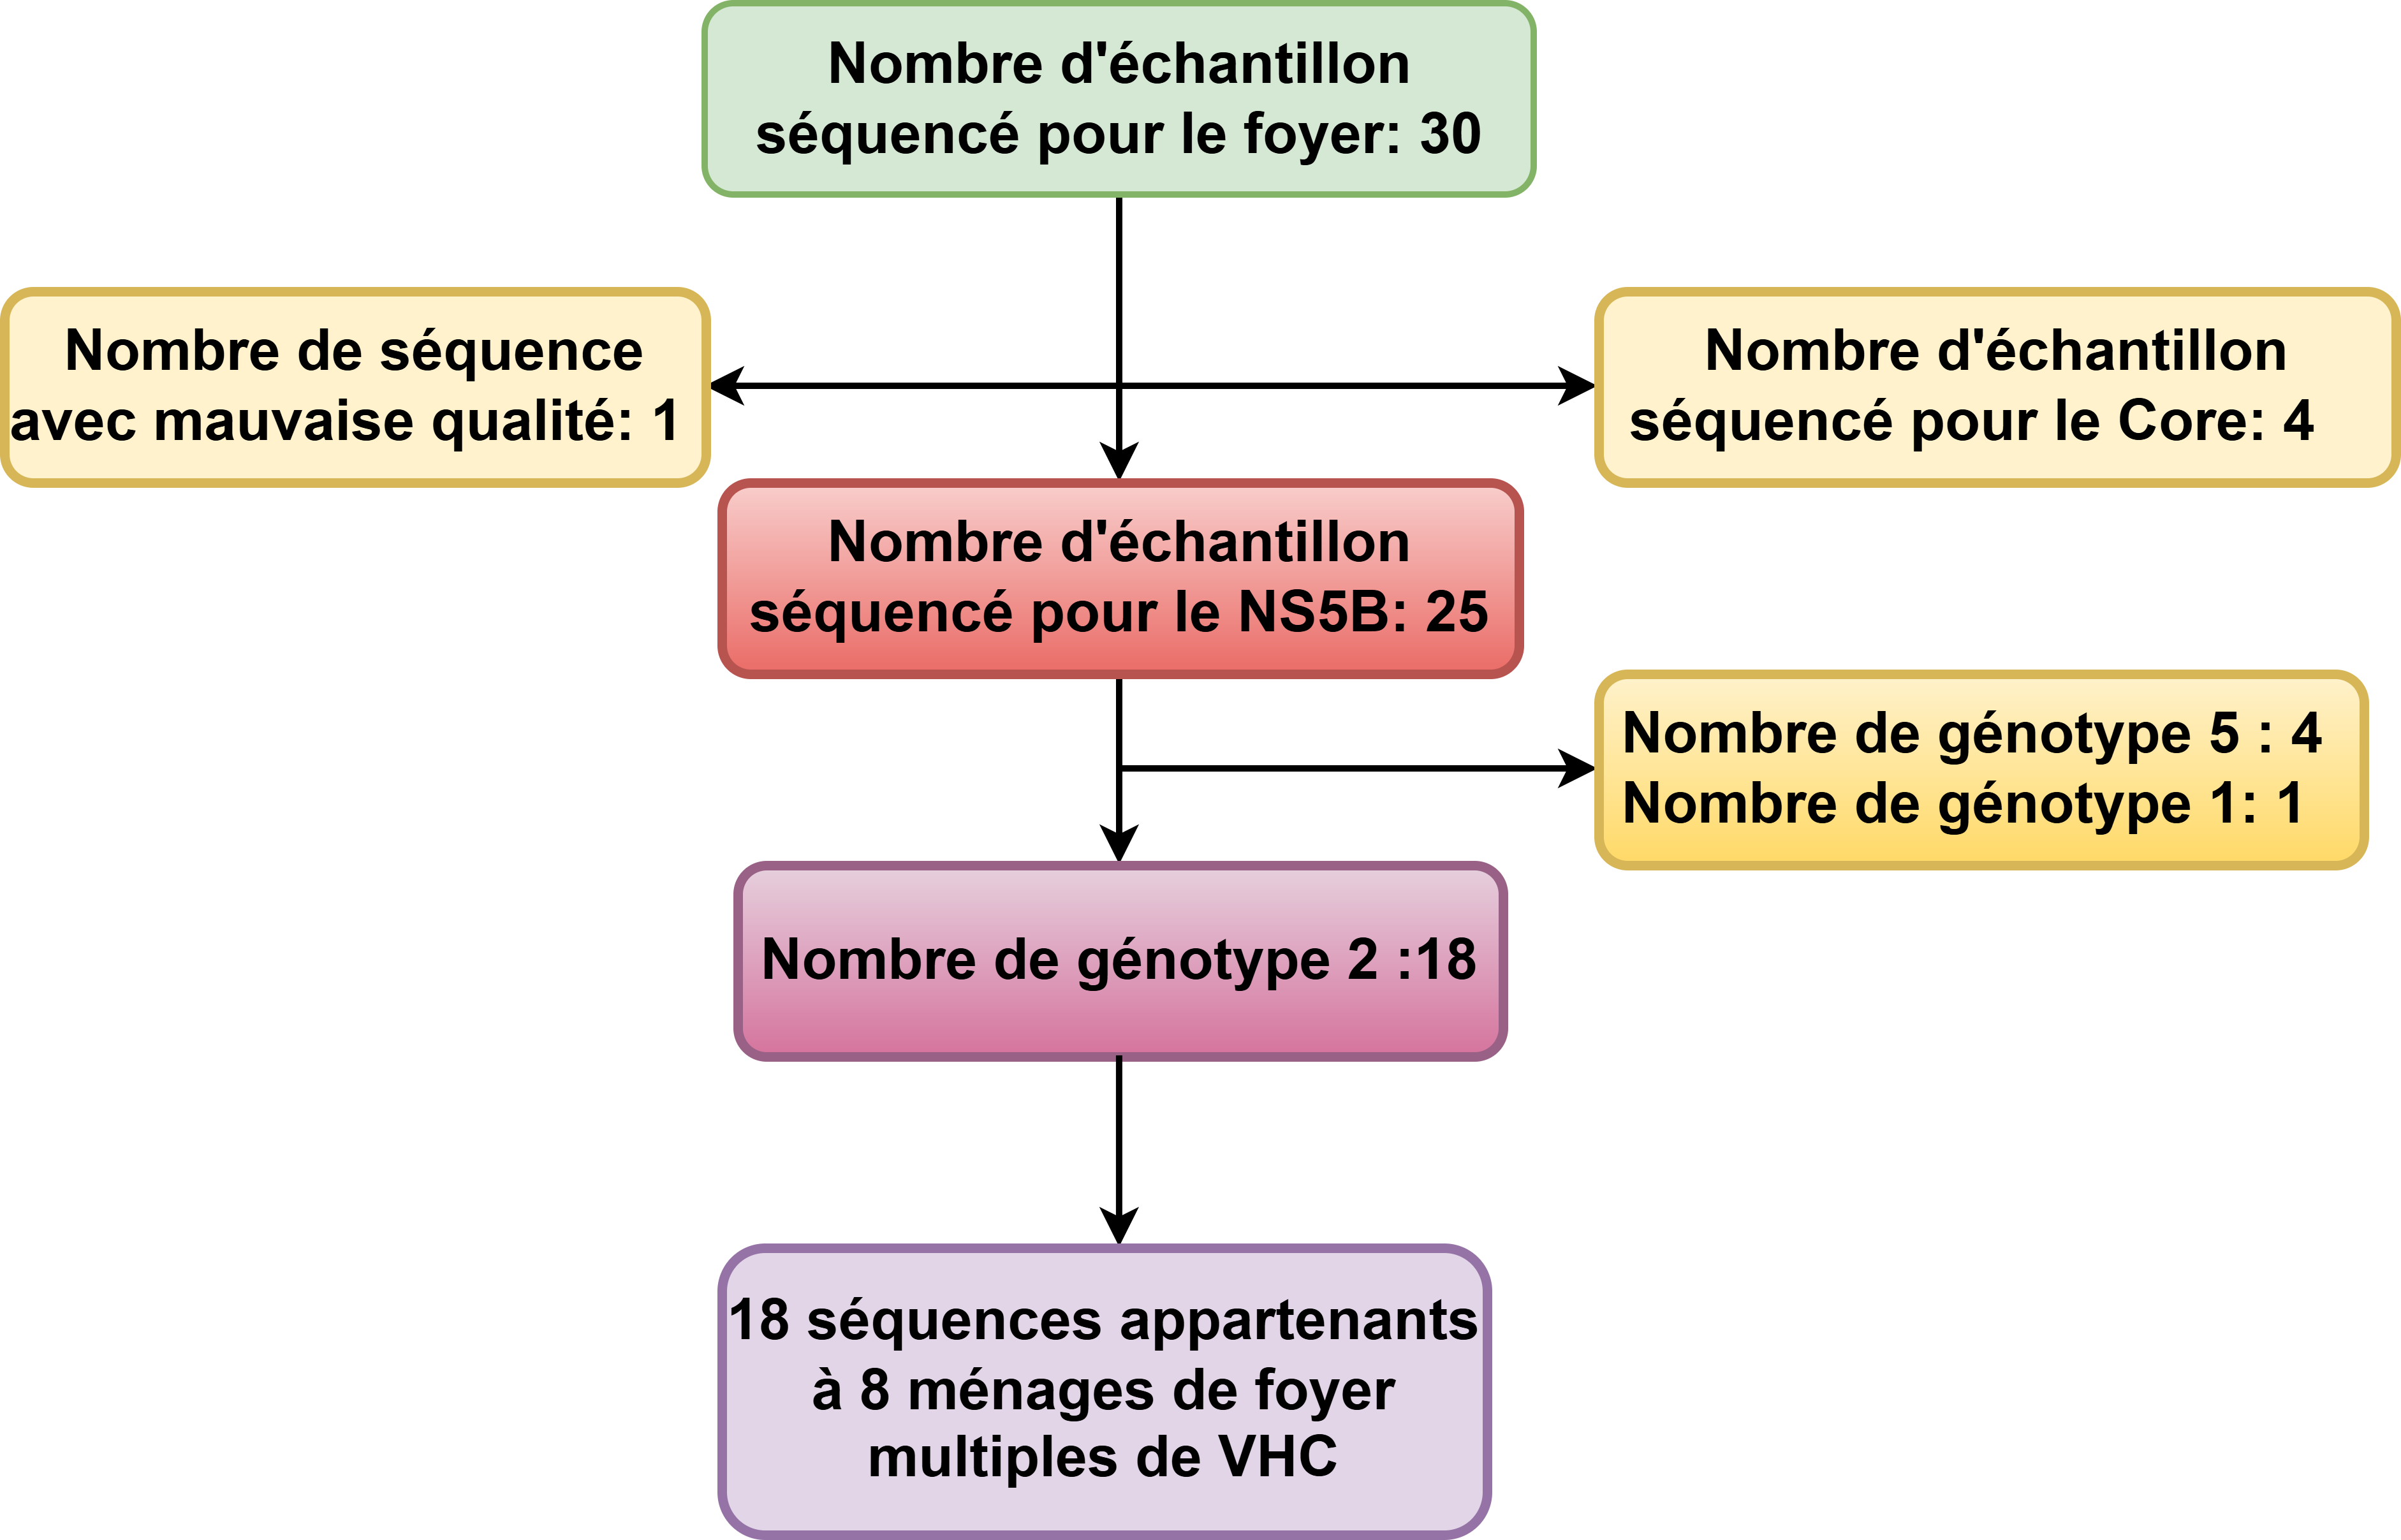
\includegraphics[width=\linewidth]{./Image/foyer.png}
        \caption{Diagramme de flux des Foyers multiples}
        \label{fig:foyer}
    \end{subfigure}
    \hfill
    \begin{subfigure}{0.48\textwidth}
        \centering
        \includegraphics[width=\linewidth]{./Image/contrle.png}
        \caption{Diagramme de flux des contrôles}
        \label{fig:controle}
    \end{subfigure}

    \caption{Diagramme de flux des participants}
    \label{fig:deux_figures}
\end{figure}



\subsection{Statistique descritives des participants}
L'âge médian des participants du groupe des foyers multiples étaient de 40 ans avec un intervale interquartile (IIQ) de [18-57,5] ans, et 38,89 \% étaient des femmes. Dans le groupe contrôle, l'âge médian était de 44 ans avec un IIQ de [31-60] ans, et 59,57\% étaient des femmes (tableau \ref{tab: caracteristiques}).

\begin{table}[!htbp]
\centering
\caption [Statistiques descriptives des participants] {Statistiques descriptives des participants selon lle groupe (foyer multiple et contrôle)}
\label{tab:caracteristiques}

\begin{tabular}{>{\raggedright\arraybackslash}p{5cm}
                >{\raggedleft\arraybackslash}p{4cm}
                >{\raggedleft\arraybackslash}p{4cm}}
\toprule
\textbf{Variables} &
\centering\textbf{Foyers multiples}\\(n = 18)\\N (\%) ou médiane [IIQ] &
\centering\textbf{Groupe contrôle}\\(n = 47)\\N (\%) ou médiane [IIQ] \tabularnewline
\midrule

 \textbf{Âge (ans) }                 & 40 [18--57,5] & 44 [31--60] \\

\addlinespace
\textbf{Groupe d'âge}      &               &              \\
\hspace{0.5cm}Moins de 20 ans & 5 (27,78)    & 3 (6,38)     \\
\hspace{0.5cm}Plus de 20 ans  & 13 (72,22)   & 44 (93,62)   \\

\addlinespace
\textbf{Sexe}              &               &              \\
\hspace{0.5cm}Masculin      & 11 (61,11)    & 19 (40,43)   \\
\hspace{0.5cm}Féminin       & 7 (38,89)     & 28 (59,57)   \\

\bottomrule
\end{tabular}
\end{table}

\newpage

\subsection{Diversité virale intra-hôte du VHC}

Dans le groupe des foyers multiples, le ratio de la diversité virale intra-hôte du VHC variait de 0 à 24,29 \%, avec une médiane de 16,50\% et un IIQ [0,97-18,45], témoignant ainsi une forte hétérogénéité entre les individus. Les ménages M01 (18,15 IIQ[18,03-18,26]), M02 (18,99 IIQ[18,57-19,87]), M07 (15,15 IIQ[13,48-16,81]) et M08 (19,69 IIQ[17,39-21,99]) présentaient des niveaux élevés de diversité chez la plupart des participants, tandis que les ménages M03  (0,64 IIQ[0,48-0,80])et M04 (0 IIQ[0-0]) étaient caractérisés par une faible proportion de sites ambigus, traduisant des populations virales plus homogènes. En revanche, les ménages M05 (10,63 IIQ[6,75-14,50]) et M06 (1 IIQ[0,50-10,38]) montraient une variabilité plus importante entre leurs membres, suggérant des dynamiques évolutives distinctes ou des durées d'infection différentes (figure ~\ref{fig:DVF}).
\newpage
\begin{figure}[h]
\centering
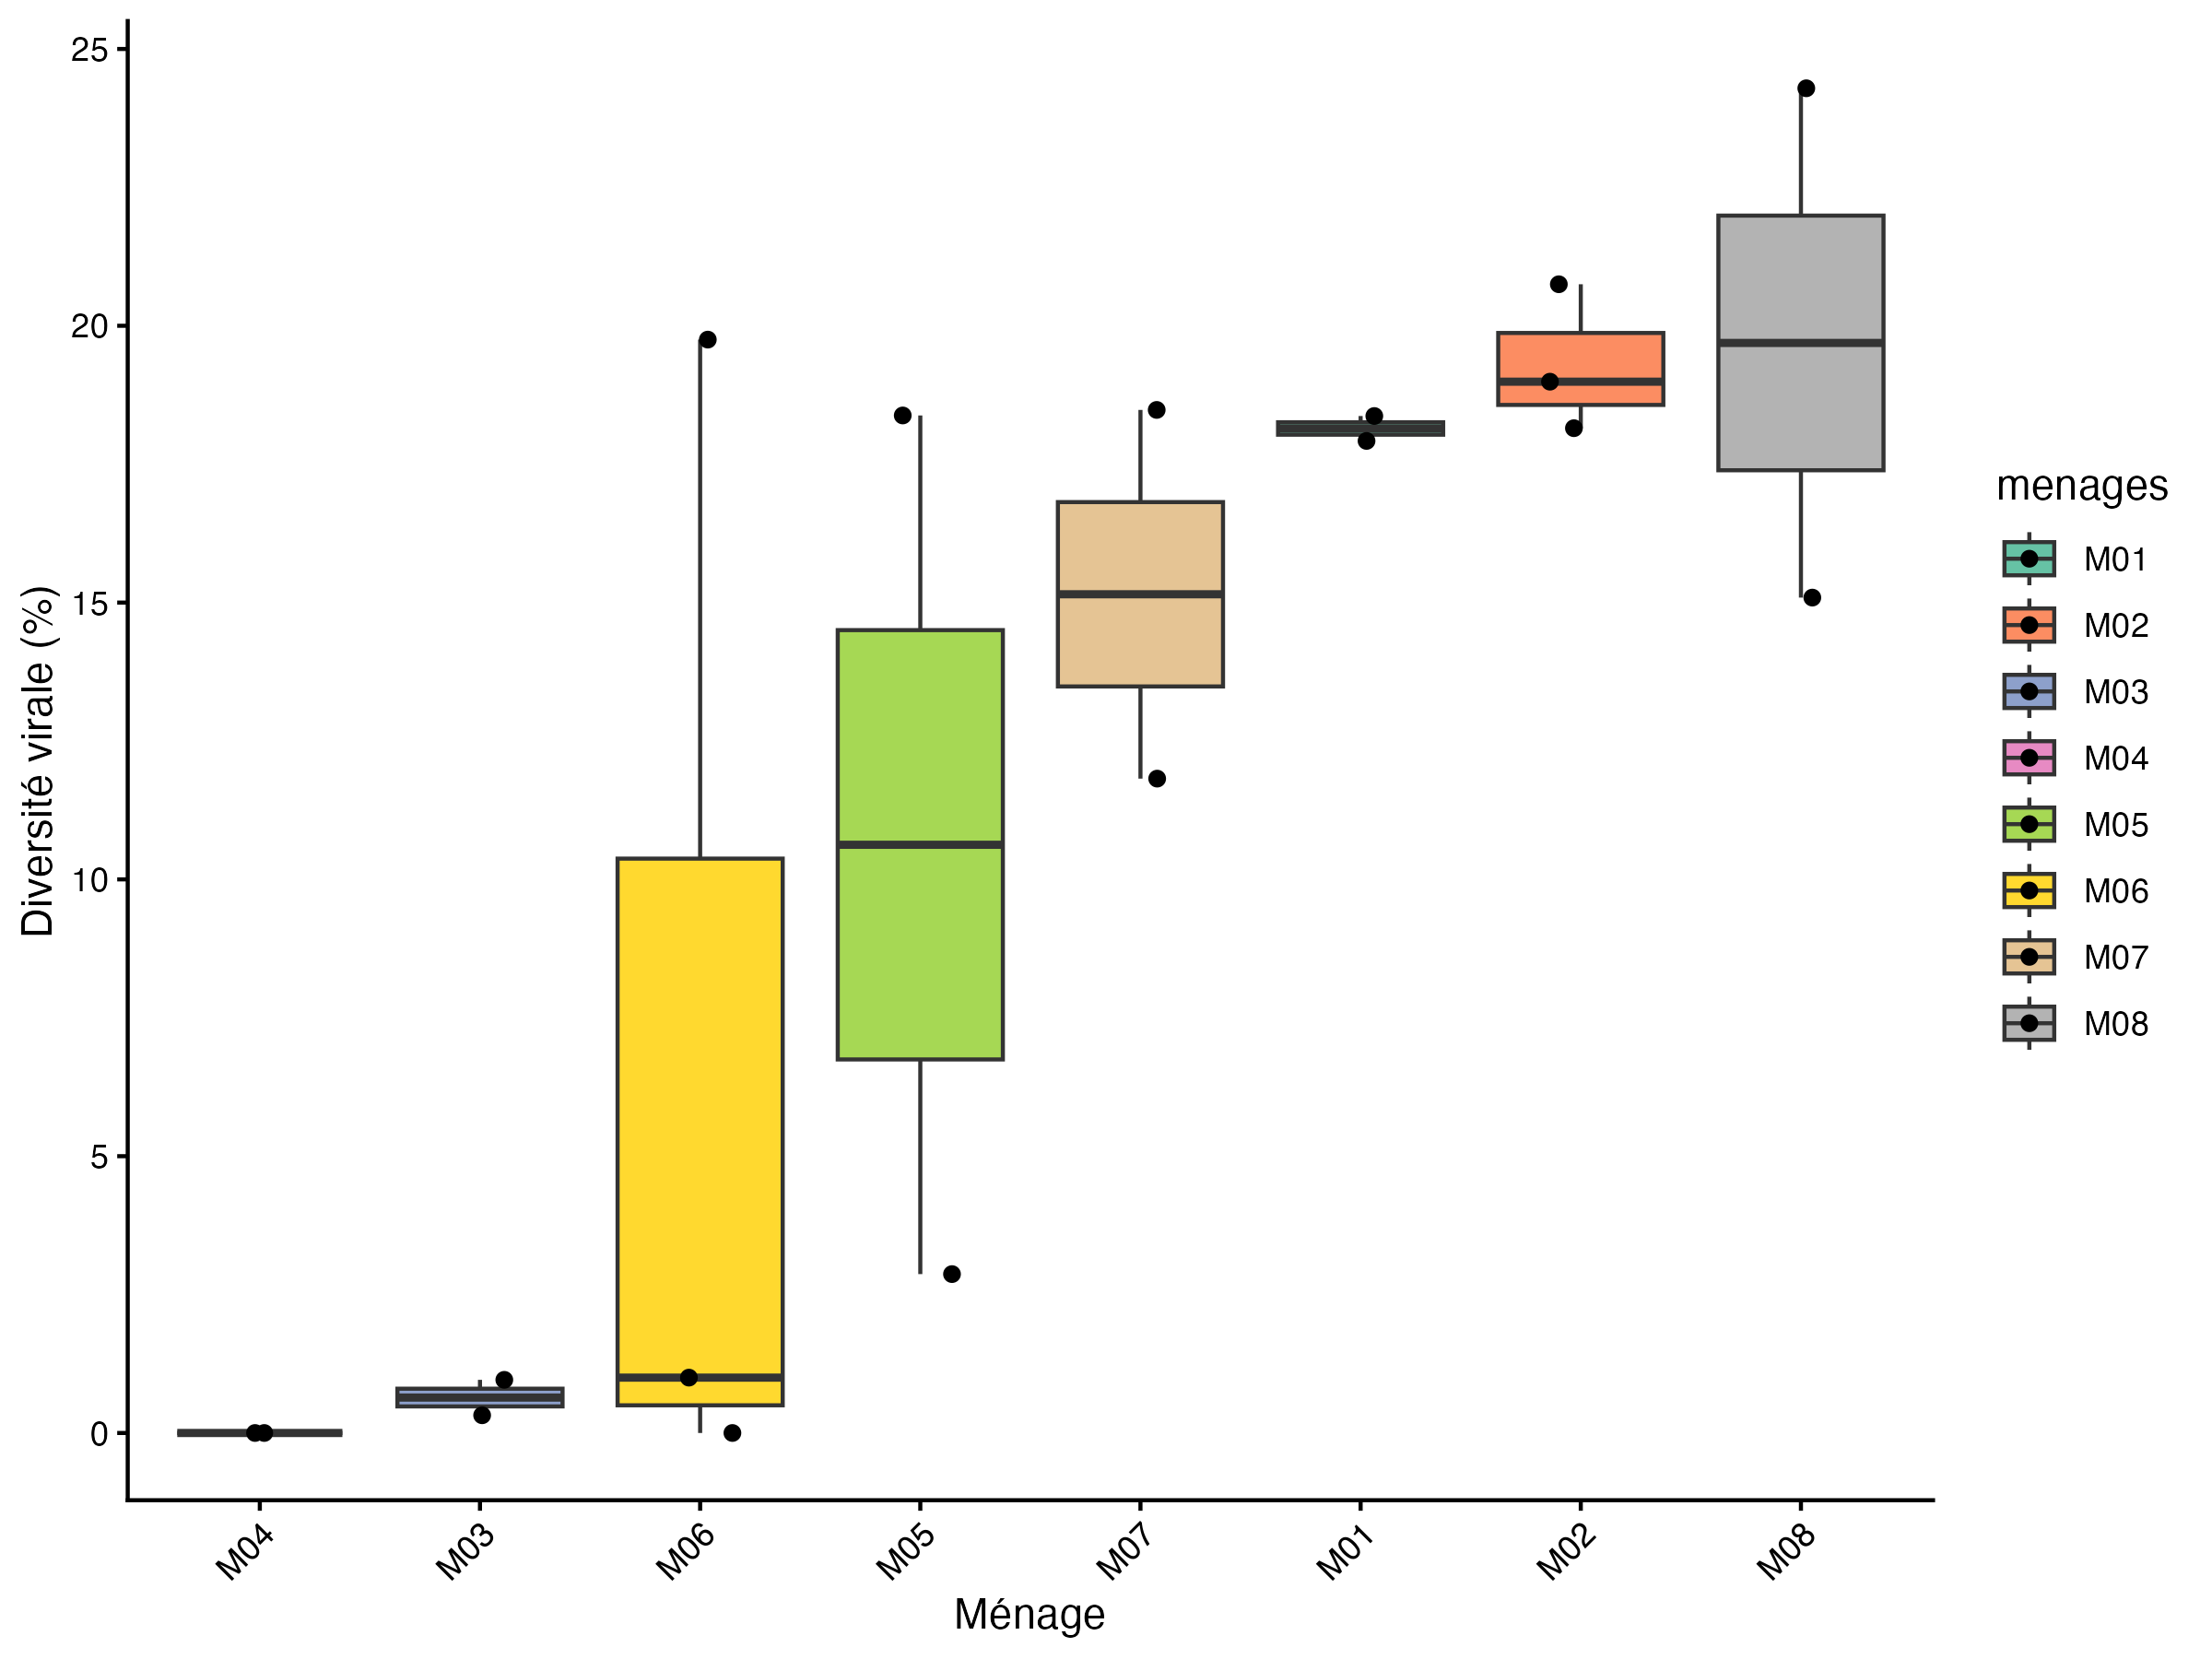
\includegraphics[width=1.15\textwidth]{./Image/diversitviralFoyer.png}
\caption [Diversité virale intra-hôte du VHC dans les foyers multiples] {Diversité virale intra-hôte du VHC dans les foyers multiples: sur ce graphe, l’axe des abscisses correspond aux ménages, distingués par des couleurs différentes, et l’axe des ordonnées au ratio de diversité virale (formule à la page \pageref{14}). La figure présente, pour chaque ménage, une boîte à moustaches illustrant la diversité virale intra-hôte, accompagnée de nuages de points représentant le nombre d’individus par ménage. À titre d’exemple, trois points sont observés pour le ménage M06, indiquant la présence de trois individus, tandis que le ménage M01 en compte deux. La boîte à moustaches décrit la distribution de la diversité virale. On observe que le ménage M08 présentait des niveaux élevés de diversité chez la majorité des participants (19,69 ; IIQ [17,39–21,99]), contrairement au ménage M06 (1 ; IIQ [0,50–10,38]), qui montrait une variabilité plus marquée entre ses membres}
\label{fig:DVF}
\end{figure}
\newpage

Dans le groupe contrôle, le ratio de la diversité intra-hôte variait de 0,31 à 11,36 \%, avec une médiane de 1,86 \% et un IIQ de [0,95-2,90] ce qui suggère une population virale plus homogènes et une faible hétérogénéité de la diversité virale du VHC, possiblement en faveur d’une infection plus récente ou une dynamique de transmission spécifique (figure ~\ref{fig:DVC}).

\begin{figure}[h]
\centering
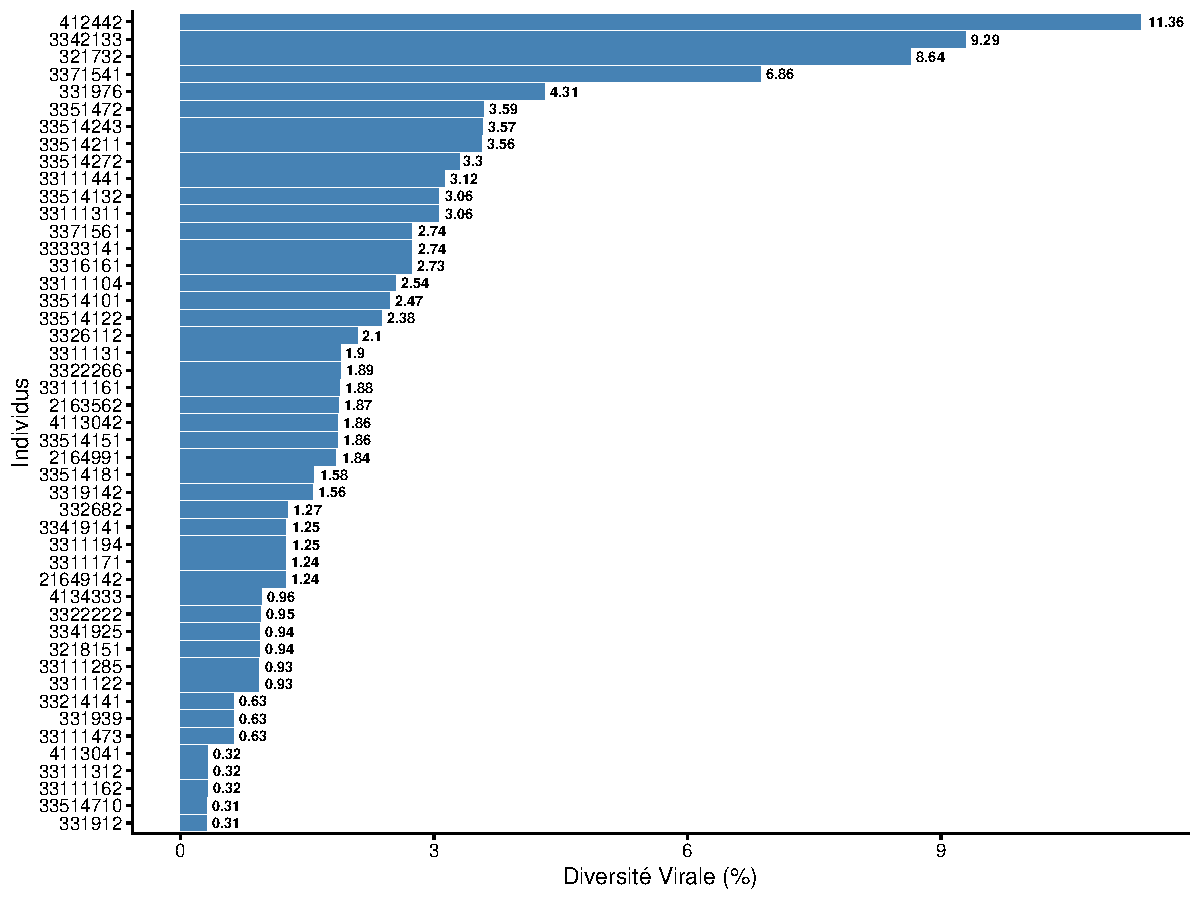
\includegraphics[width=1.1\textwidth]{./Image/diversiteviraleControle.pdf}
\caption [Diversité virale intra-hôte du VHC dans le groupe contrôle] {Diversité virale intra-hôte du VHC dans le groupe contrôle: sur l’axe des abscisses figure le ratio de diversité virale, tandis que l’axe des ordonnées présente les individus, identifiés par leur numéro d’identifiant. Cette figure illustre la diversité intra-hôte du VHC chez chaque individu. Pour l'identifiant \textbf{331912}, la diversité intra-hote est de \textbf{0,31\%} qui peut être compatible avec une infection récente,le virus n’ayant pas encore eu suffisamment de temps pour accumuler des mutations. En revanche, l'identifiant \textbf{412442}, la diversité intra-hôte est de \textbf{11,36\%}, peut suggérer une infection plus ancienne, laissant davantage de temps au virus pour évoluer et muter.}
\label{fig:DVC}
\end{figure}

La comparaison de la diversité intra-hôte du VHC entre les deux groupes, le test de wilcoxon à montré une différence statistiquement significative avec une p-value de 0,02 (figure ~\ref{fig:compare}).

 \newpage

\begin{figure}[h]
\centering
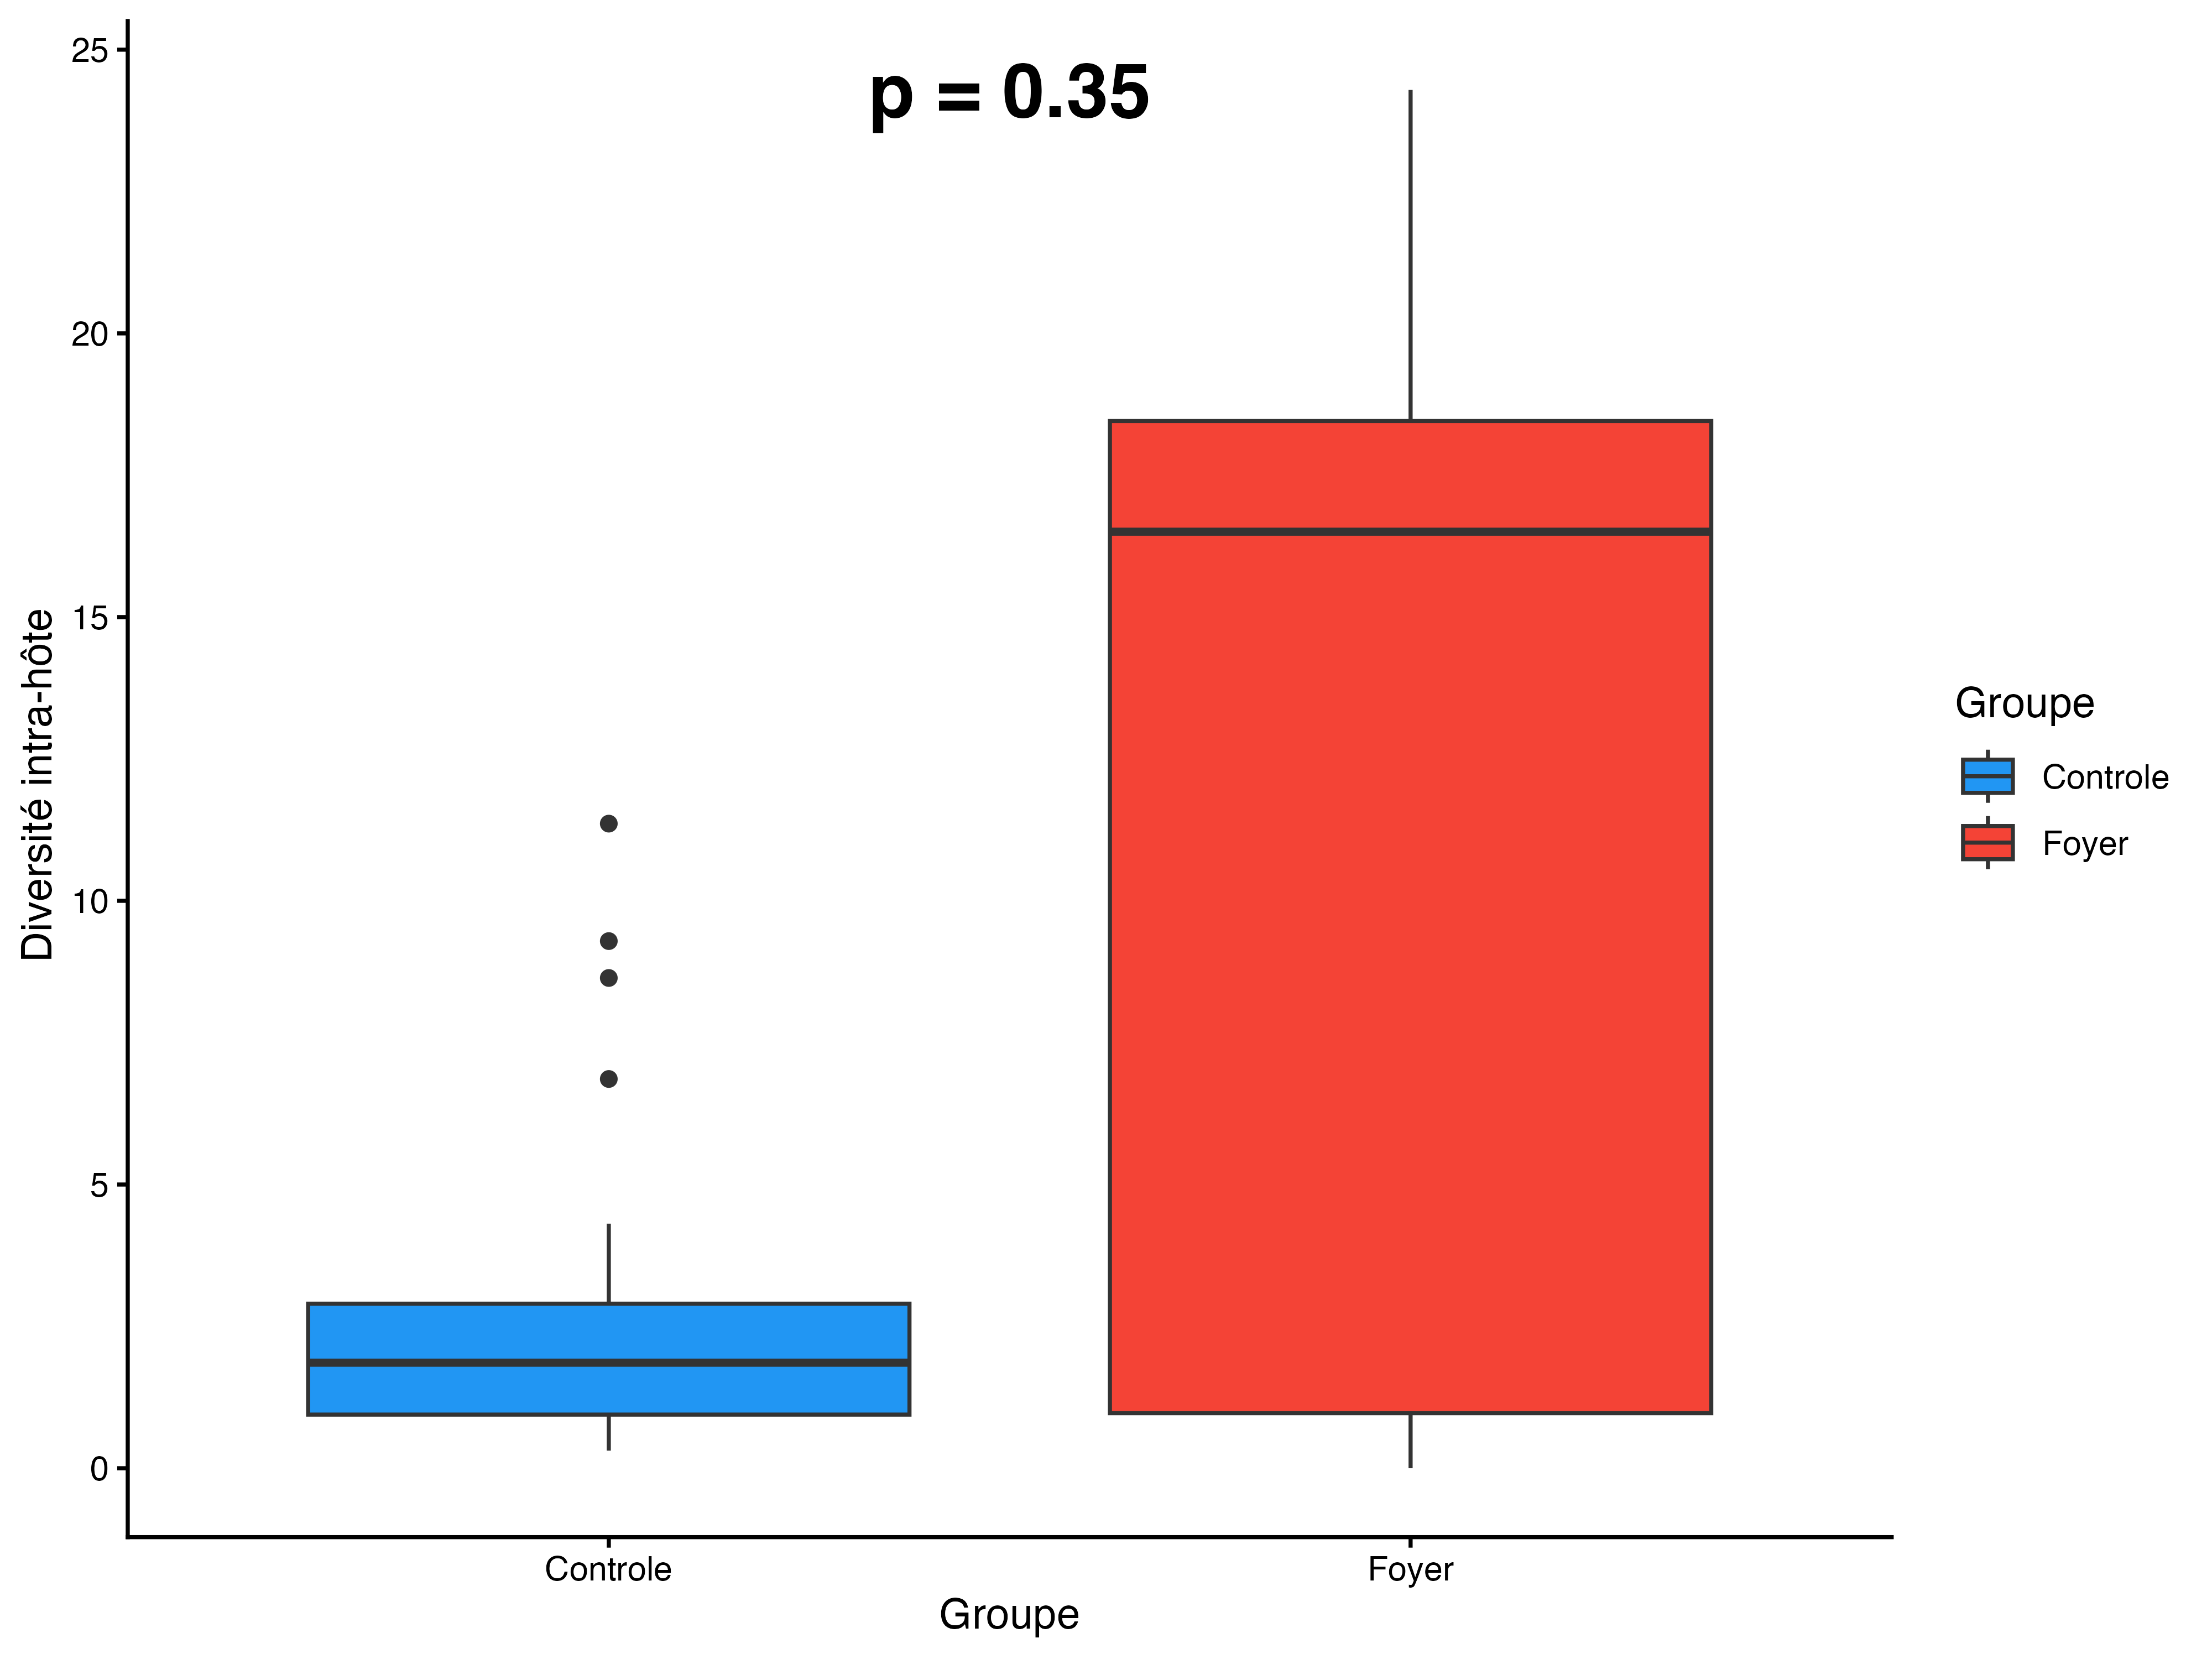
\includegraphics[width=1.18\textwidth]{./Image/diversitefoyercontrole.png}
\caption [Distribution de la diversité intra-hôte du VHC] {Comparaison de la distribution de la diversité intra-hôte du VHC des deux groupes: Cette figure compare la distribution de la diversité intra-hôte du VHC entre deux groupes, à savoir les foyers multiples, représentés en rouge, et le groupe contrôle, représenté en bleu. L’axe des abscisses correspond aux groupes, tandis que l’axe des ordonnées indique la diversité virale. La boîte à moustaches montre que la médiane de la diversité est plus élevée chez les foyers multiples (16,50\%) que chez le groupe contrôle (1,86\%). Cette différence est statistiquement significative d’après le test de Wilcoxon (p-value = 0,02).

}
\label{fig:compare}
\end{figure}

\subsection{Distance génétique du VHC}

De manière globale, la distance génétique variait de 0 à 0,39, avec une médiane de 0,18 et un IIQ de [0,13-0,26]. Dans les foyer multiples, elle variait de 0 à 0,31, avec une médiane de 0,08 et un IIQ de [0,05 - 0,13], traduisant une plus grande homogénéité génétique des séquences virales. À l’inverse, dans le groupe contrôle, la distance génétique variait de 0,01 à 0,38, avec une médiane autour de 0,24 et un IIQ de [0,17-0,28], indiquant une diversité génétique plus élevée. \\


La comparaison entre les deux groupes à l’aide du test de Wilcoxon a montré une différence statistiquement significative (p < 0,05). Cette différence pourrait s’expliquer par une circulation virale plus importante au sein des foyers multiples, possiblement une transmission d'origine commune ou intrafamiliale.

\subsection{Catégorisation de la transmission du VHC dans les foyers multiples}

Au total, les 18 séquences issues des foyers multiple ont permis 153 comparaisons par distance génétique, dont 12 comparaisons intra-foyer et 141 comparaisons inter-foyer. Les distances génétiques inter-foyer présentaient une médiane de 0,22 [0,14–0,26], tandis que les distances intra-foyer avaient une médiane de 0,19 [0,03–0,28]. Bien que les distances intra-foyer soient légèrement plus faibles, la comparaison entre les deux distributions à l’aide du test de Wilcoxon/Mann-Whitney n’a pas mis en évidence de différence statistiquement significative (p = 0,34) (figure ~\ref{fig:compare2}). 
\newpage
\begin{figure}[h]
\centering
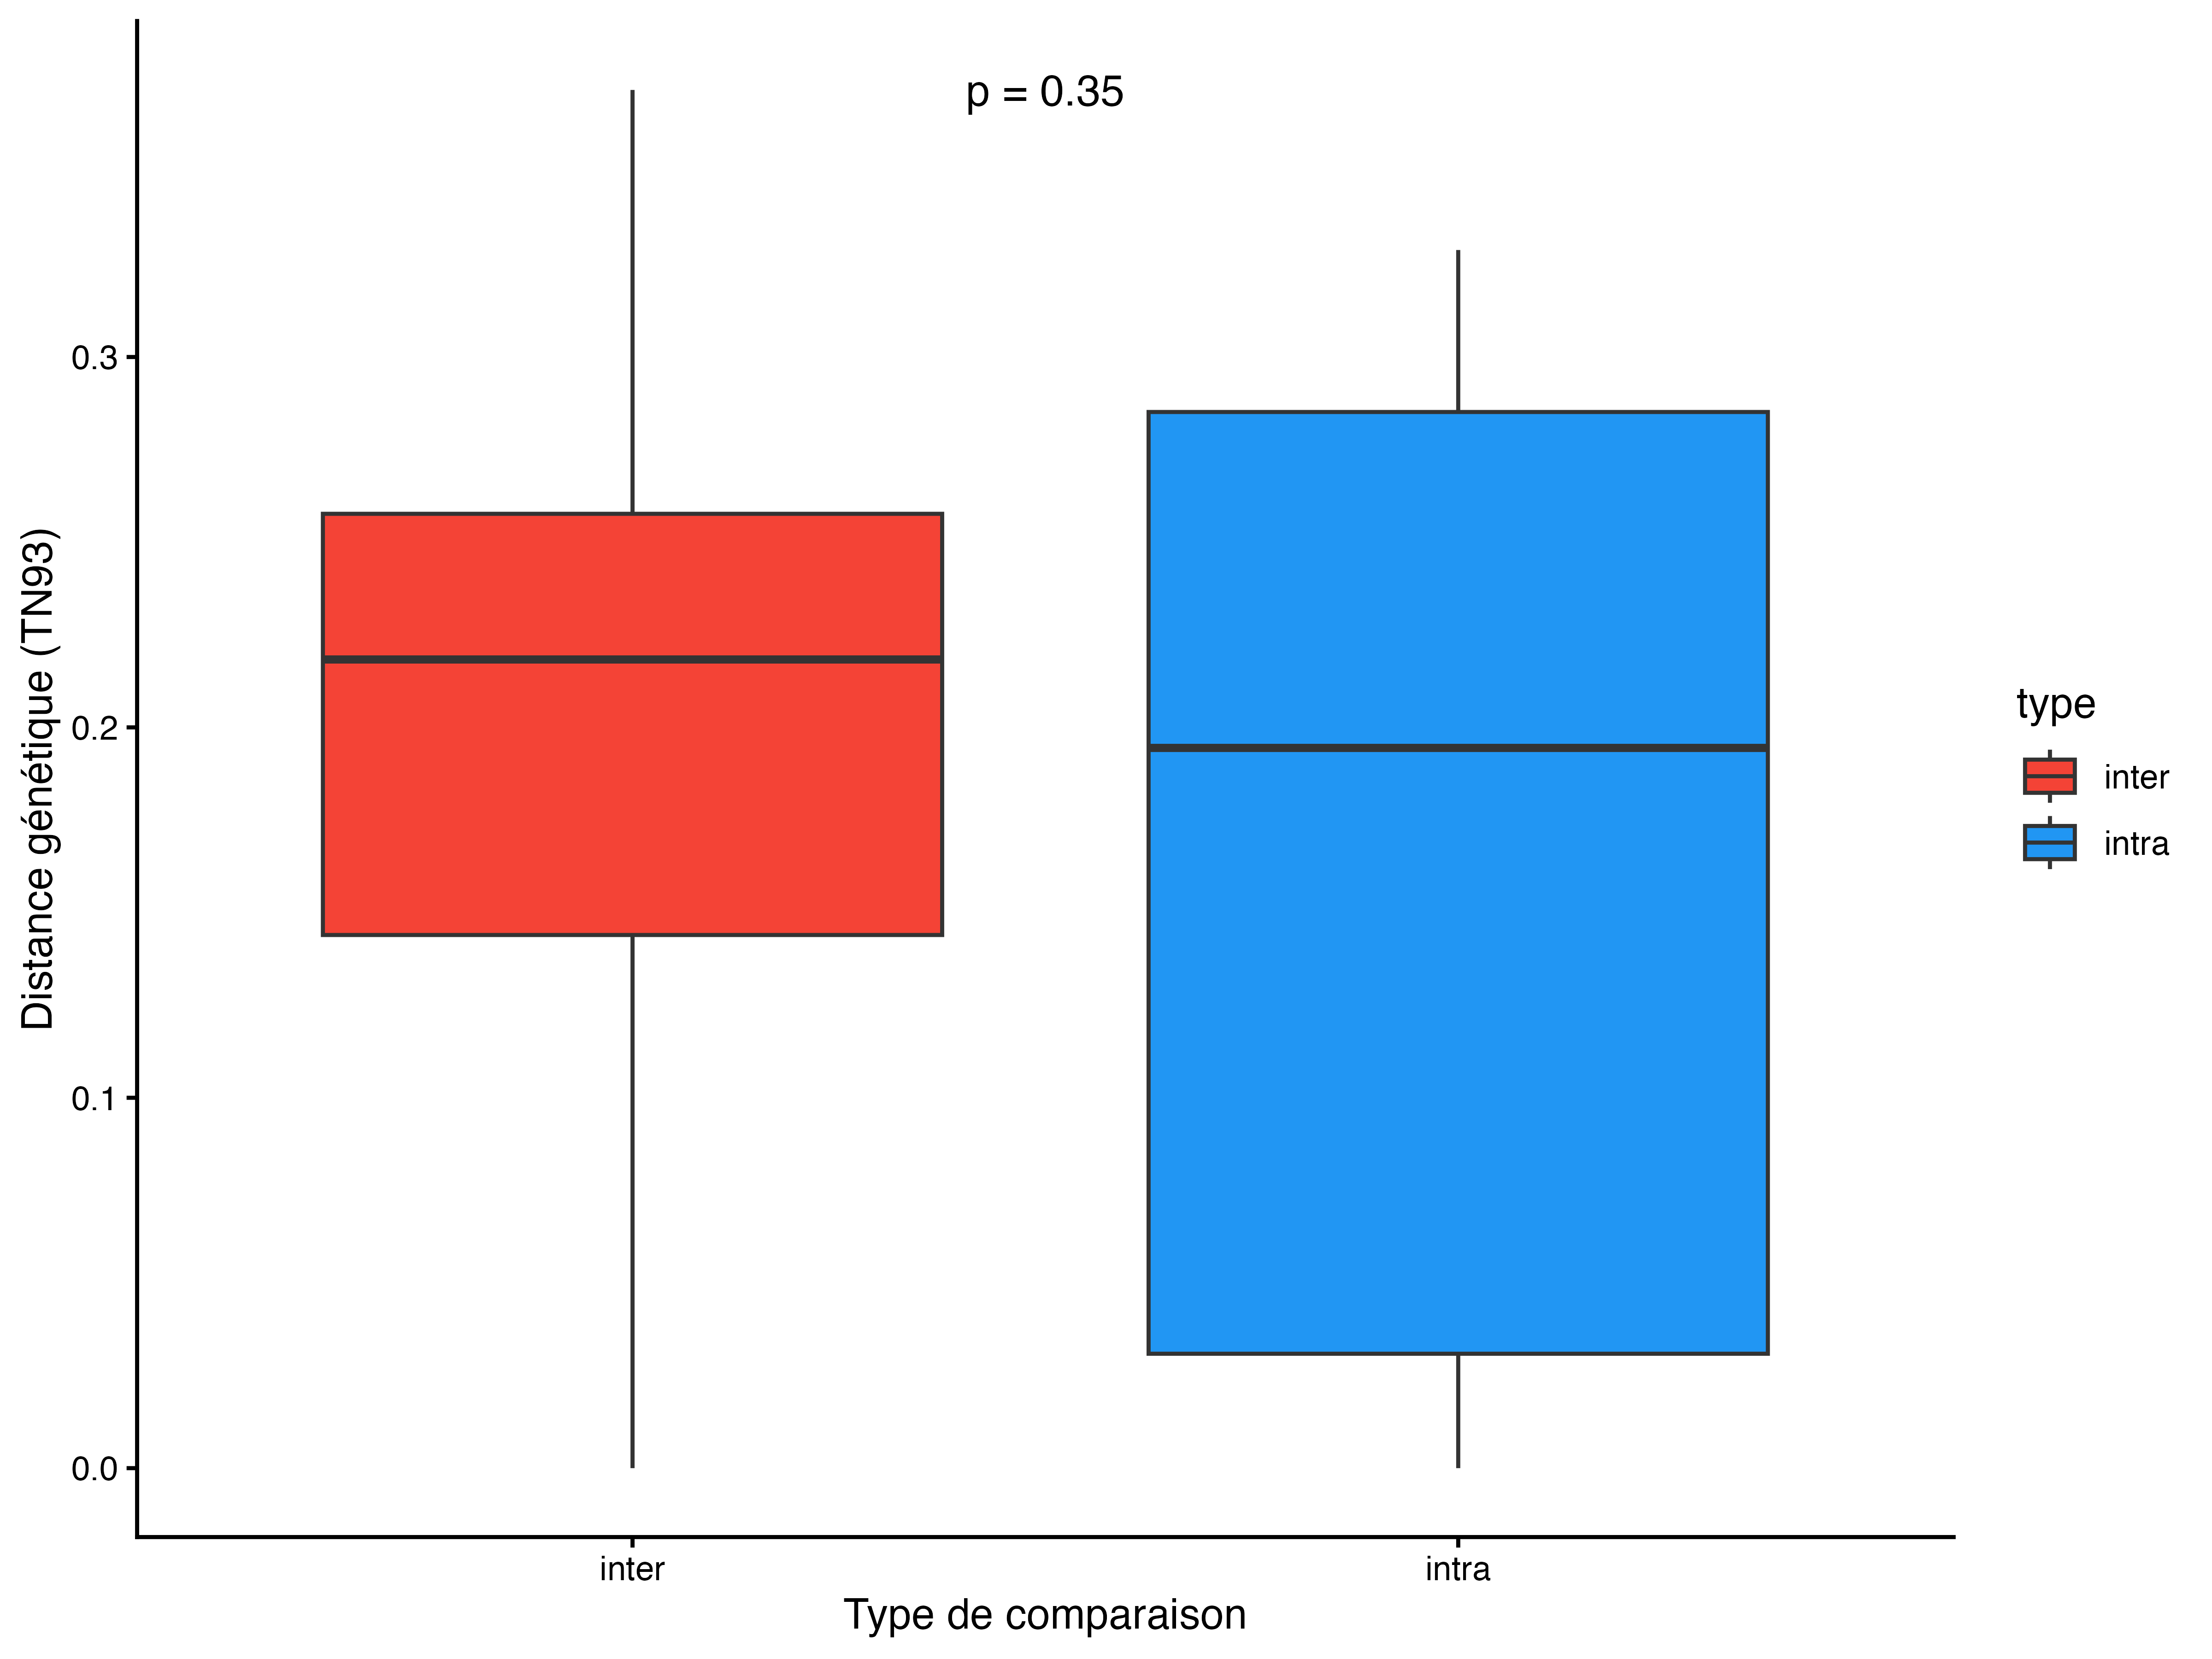
\includegraphics[width=1\textwidth]{./Image/boxplot_intra_inter.png}
\caption [Distribution de la distance génétique du VHC dans les foyers multiples ]{Comparaison de la distribution de la distance génétique dans les foyers multiples (intra et inter)}
\label{fig:compare2}
\end{figure}

À partir de la carte de chaleur, on remarque que deux individus du M06 (intra) et le M04 et M06 (inter)  ont une distance génétique très faible (0) (couleur claire: jaune). En plus de cela, on a une distance génétique observée entre M02-2110425 et M06-3322291 (inter) est très faible (0,0096), traduisant une forte similarité entre les deux séquences virales et une proximité phylogénétique marqué (figure ~\ref{fig:matrice}). Tout cela pourrait s'explique soit par une transmission intra-ménage probable, soit une source commune d'infection, soit une circulation de souches virales commune ou une transmission entre foyers.  Ainsi, ces résultats ne fournissent pas d’argument suffisant pour confirmer une transmission intrafamiliale globale dans les foyers multiples. 
\newpage
\begin{figure}[h]
\centering
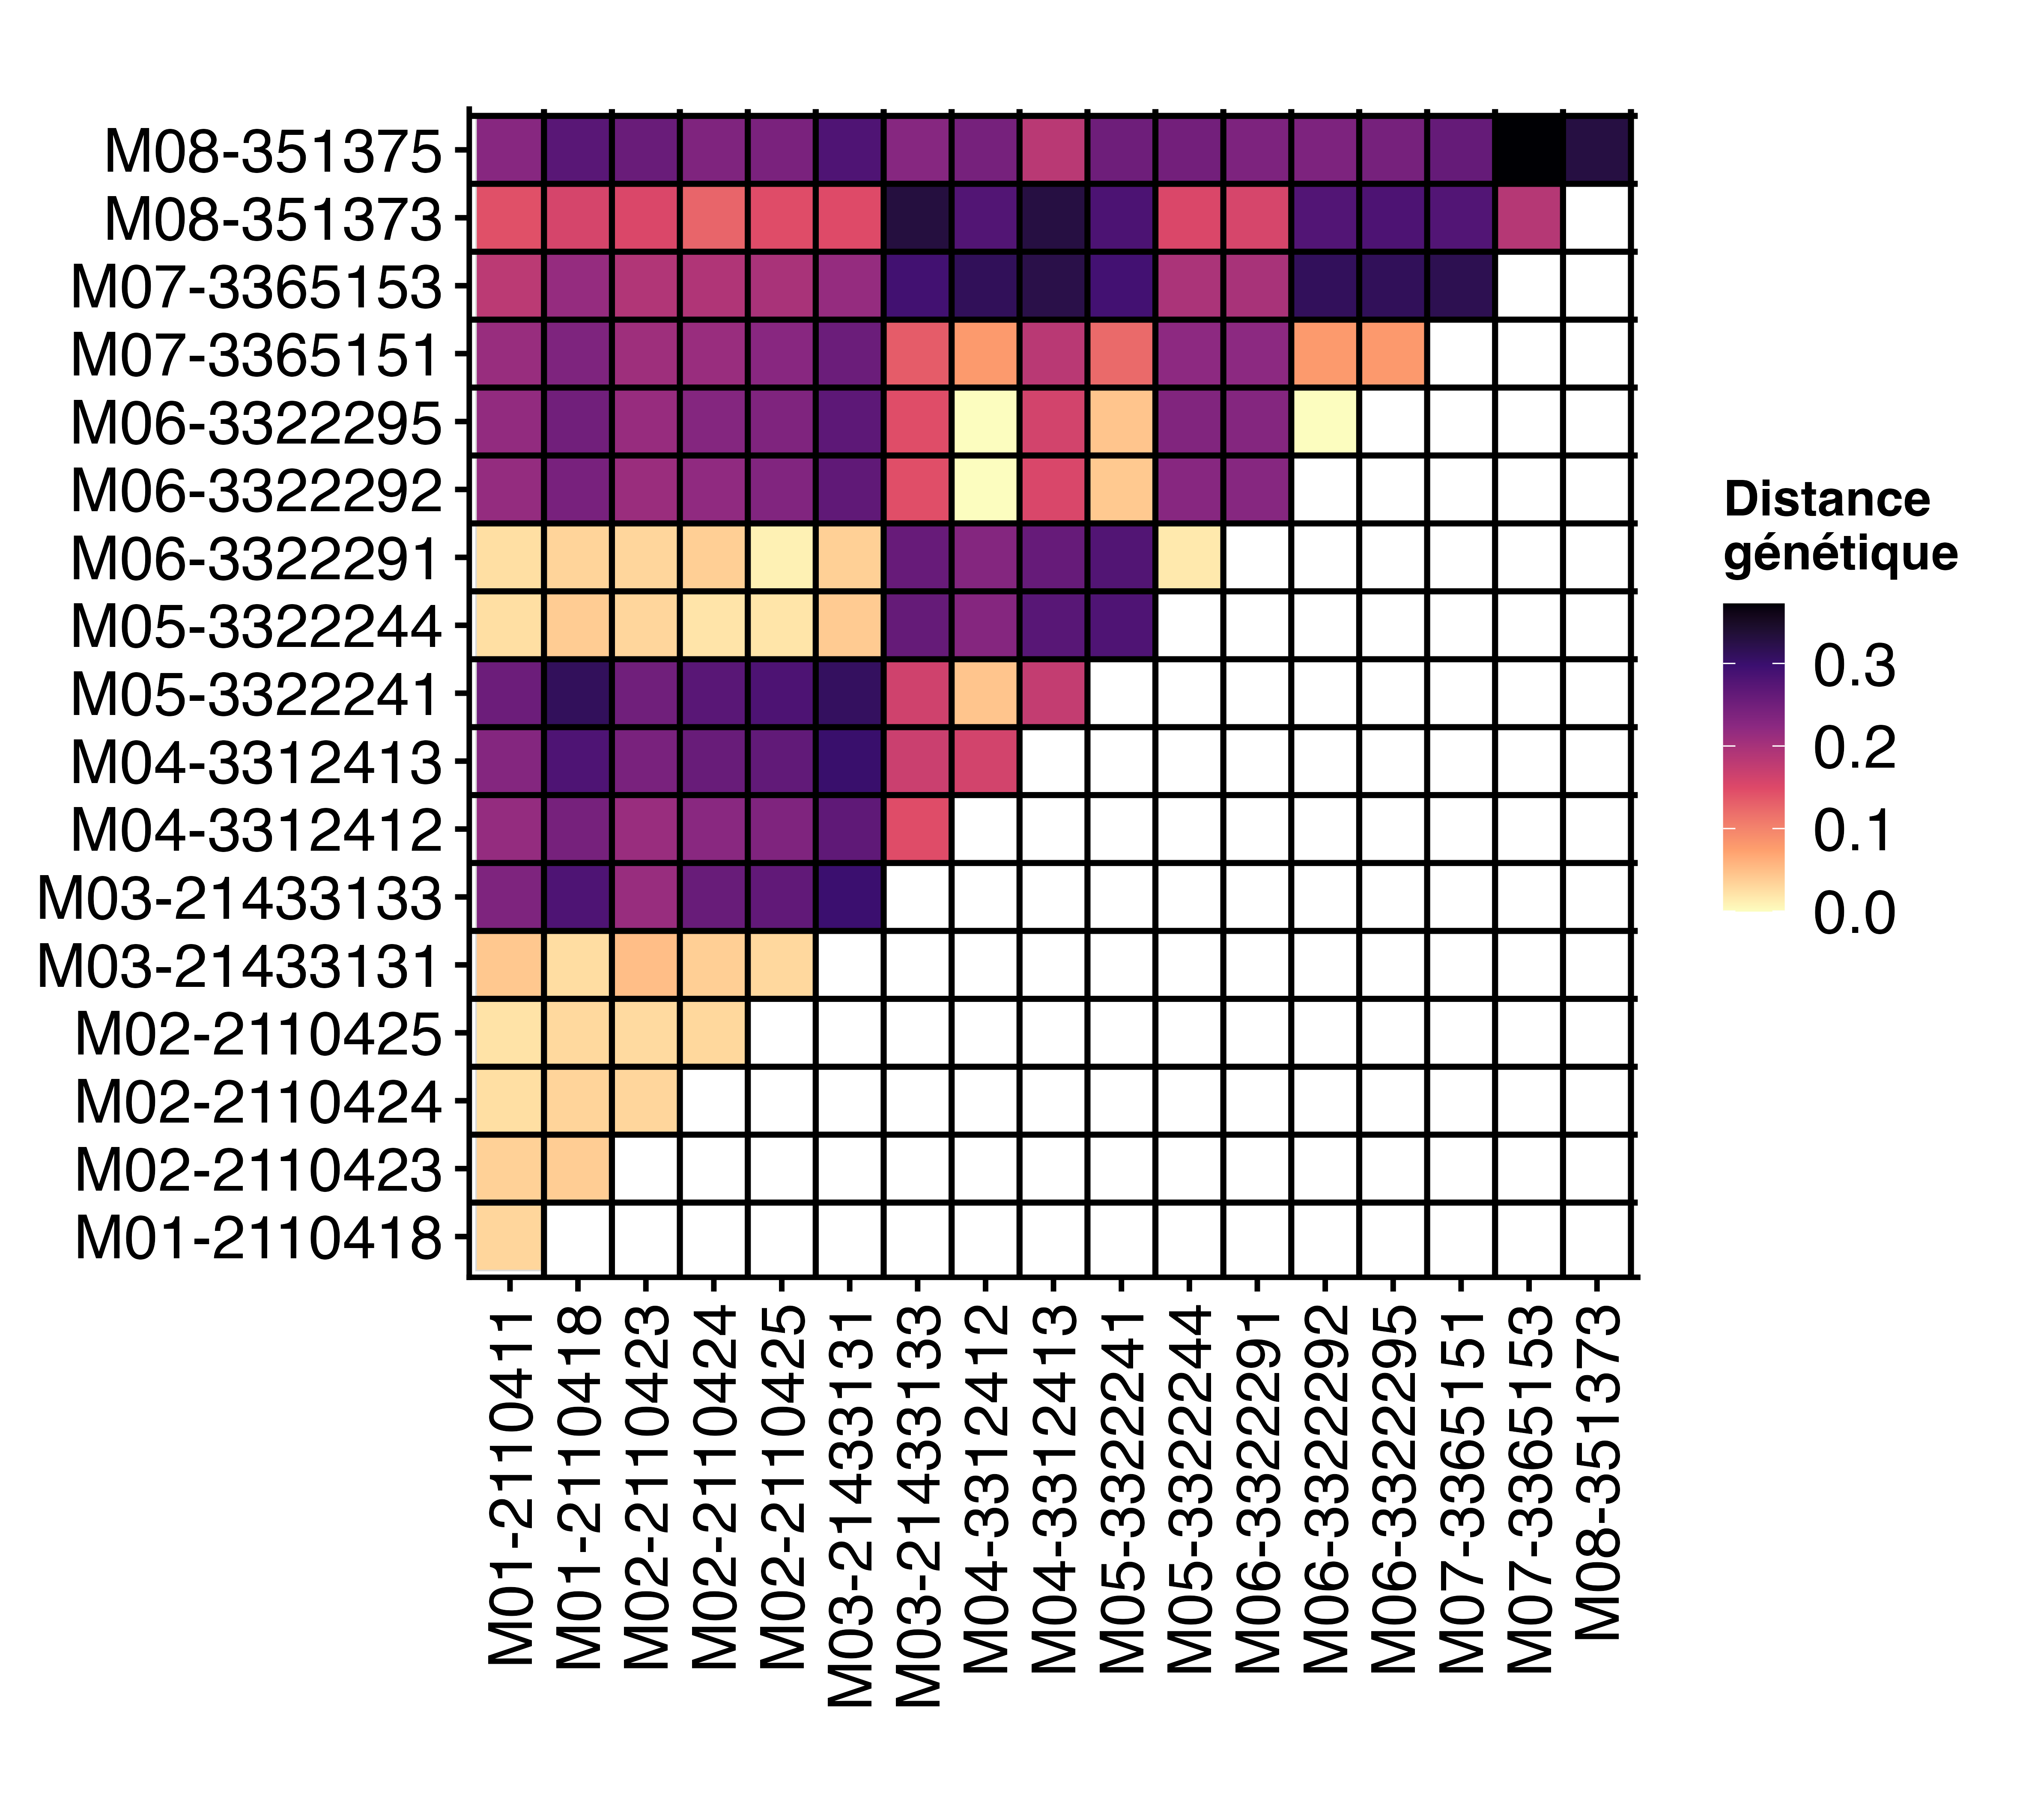
\includegraphics[width=1.15\textwidth]{./Image/heatmap_distancesfoyerprimary2.png}
\caption{Matrice de la distance génétique dans les Foyers multiples }
\label{fig:matrice}
\end{figure}

\subsection{Évènement de transmission du VHC au sein des foyers }

L’analyse des événements de transmission intraménage montre que certains foyers, notamment M01, M02 et un individus de M06, présentent des distances génétiques inférieures au seuil de 3\%, suggérant une forte proximité phylogénétique des séquences virales et une transmission intrafamiliale probable. Les distances génétiques observées dans les ménages M05, les deux individus du M06, M07 et M08, comprises entre le seuil de 3\% et le 5\textsuperscript{e} percentile, se situent dans une zone de proximité génétique faible à modérée, restant compatibles avec une similarité virale importante, mais moins convaincantes qu'une valeurs strictement inférieur à 3\%. Pour le ménage M04, dont la valeur se situe entre le 5\textsuperscript{e} percentile et la médiane, la distance génétique traduit une divergence modérée. En revanche, le ménage M03, caractérisé par une distance plus élevée, suggère une moindre proximité génétique des séquences virales, ce qui est moins compatible avec une transmission intraménage et pourrait refléter une origine distincte des infections ou une source commune non identifiée (figure ~\ref{fig:evenemt}).

\begin{figure}[h]
\centering
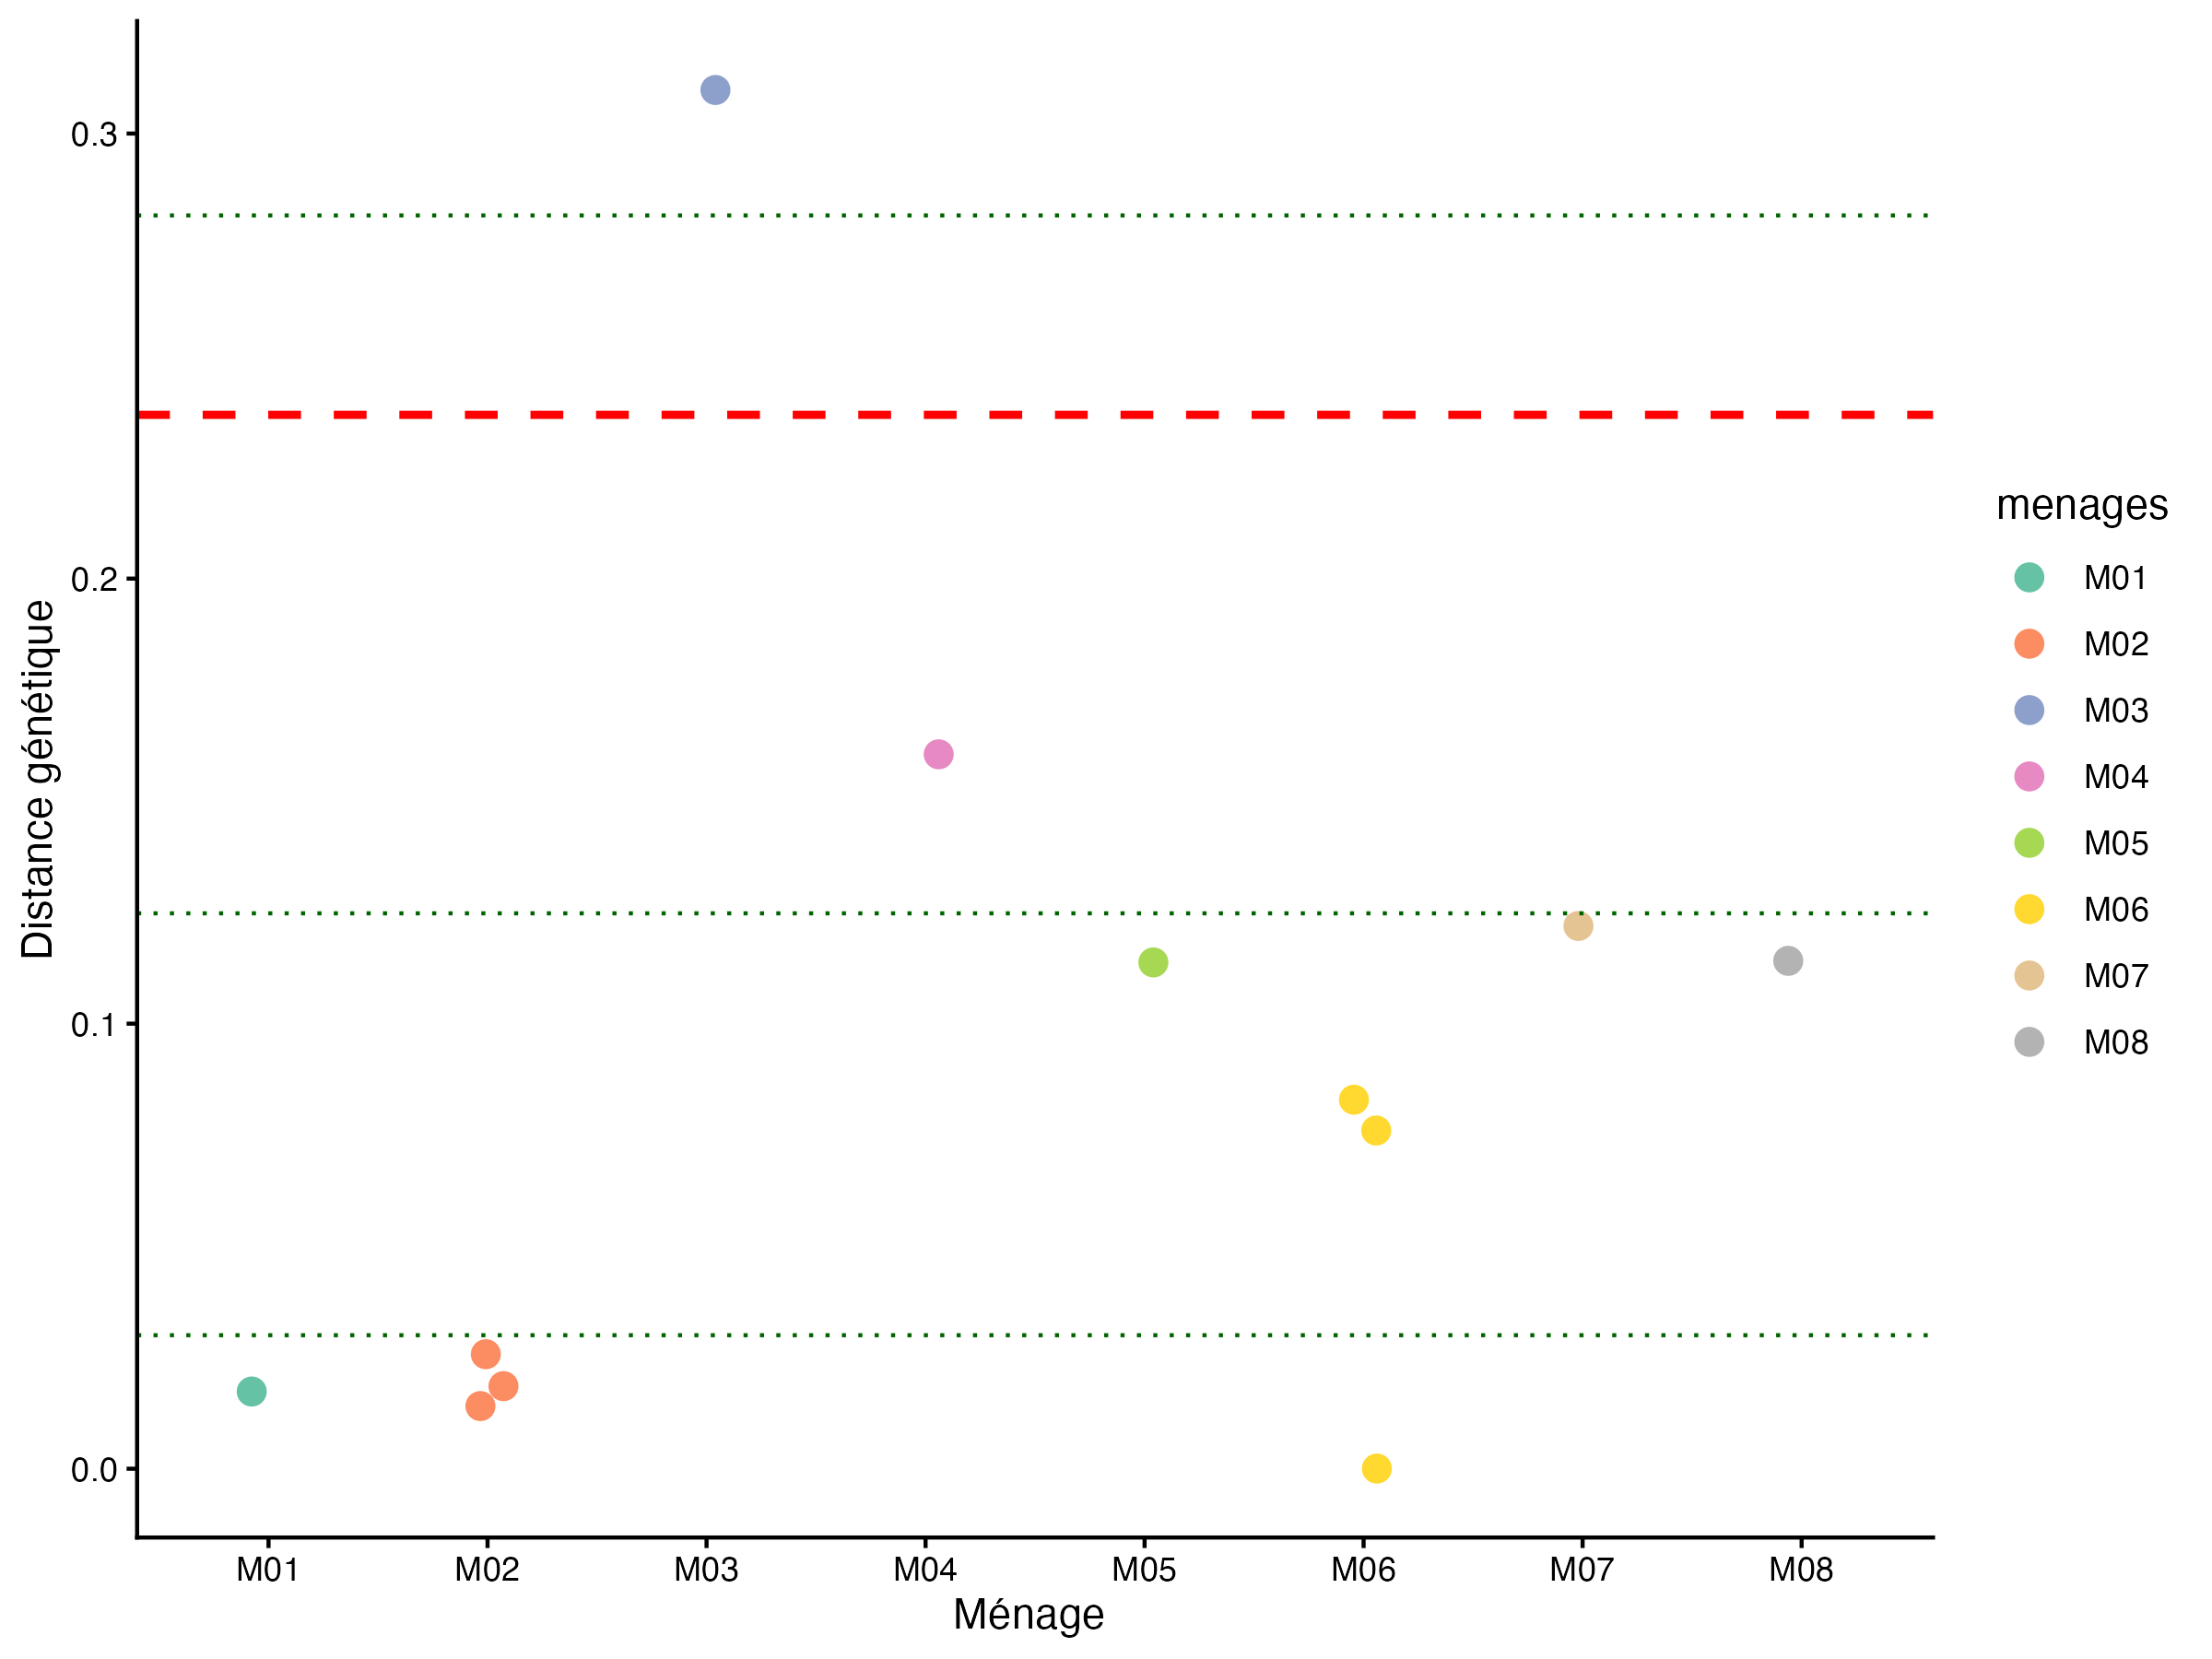
\includegraphics[width=1.15\textwidth]{./Image/evenementtransmission.png}
\caption{Évènement de la transmission du VHC dans les foyers multiples}
\label{fig:evenemt}
\end{figure}


\subsection{Analyse phylogénétique du VHC : foyer multiple}

L’analyse phylogénétique des foyers multiples, réalisée par la méthode des distances et par la méthode du Maximum de Vraisemblance, met en évidence des regroupements partiels de séquences appartenant à un même ménage, suggérant une proximité génétique importante au sein de certains foyers. En particulier, les ménages M02 et M06, présentent des regroupements plus serrés de leurs séquences virales, compatibles avec une forte proximité génétique et une possible transmission intrafamiliale. À l’inverse, d’autres ménages, tels que M03, M05, M07 et M08, montrent une dispersion plus marquée des séquences, suggérant une plus grande hétérogénéité génétique et une transmission moins évidente (figure ~\ref{fig:foyerM}).\\
La topologie obtenue par Maximum de Vraisemblance est globalement proche de celle obtenue par la methode des distances. Plusieurs clades sont bien soutenus par des valeurs de bootstraps comprises entre 74\% et 100\%, ce qui renforce la robutesse de certains regroupements. En particulier, le clade comprenant plusieurs séquences des ménages (M01, M02, M03, M05 et M06) présente un support maximal (bootstrap = 100\%). Un autre regroupement comme M05-3322241 et M06-3322292 est fortement soutenu (bootstrap = 98\%), tandis que leur regroupement avec la séquence M04-3312412 présente un support de 93\%. Mais nous remarquons sur l'arbre que les séquences provenant d'un même ménage ne se regroupe pas strictement au sein du même clade monophélitique exclusifs figure ~\ref{fig:foyerML}), limitant ainsi la conclusion d’une transmission intrafamiliale au sein des ménages. 
 
 \newpage
\begin{figure}[h]
\centering
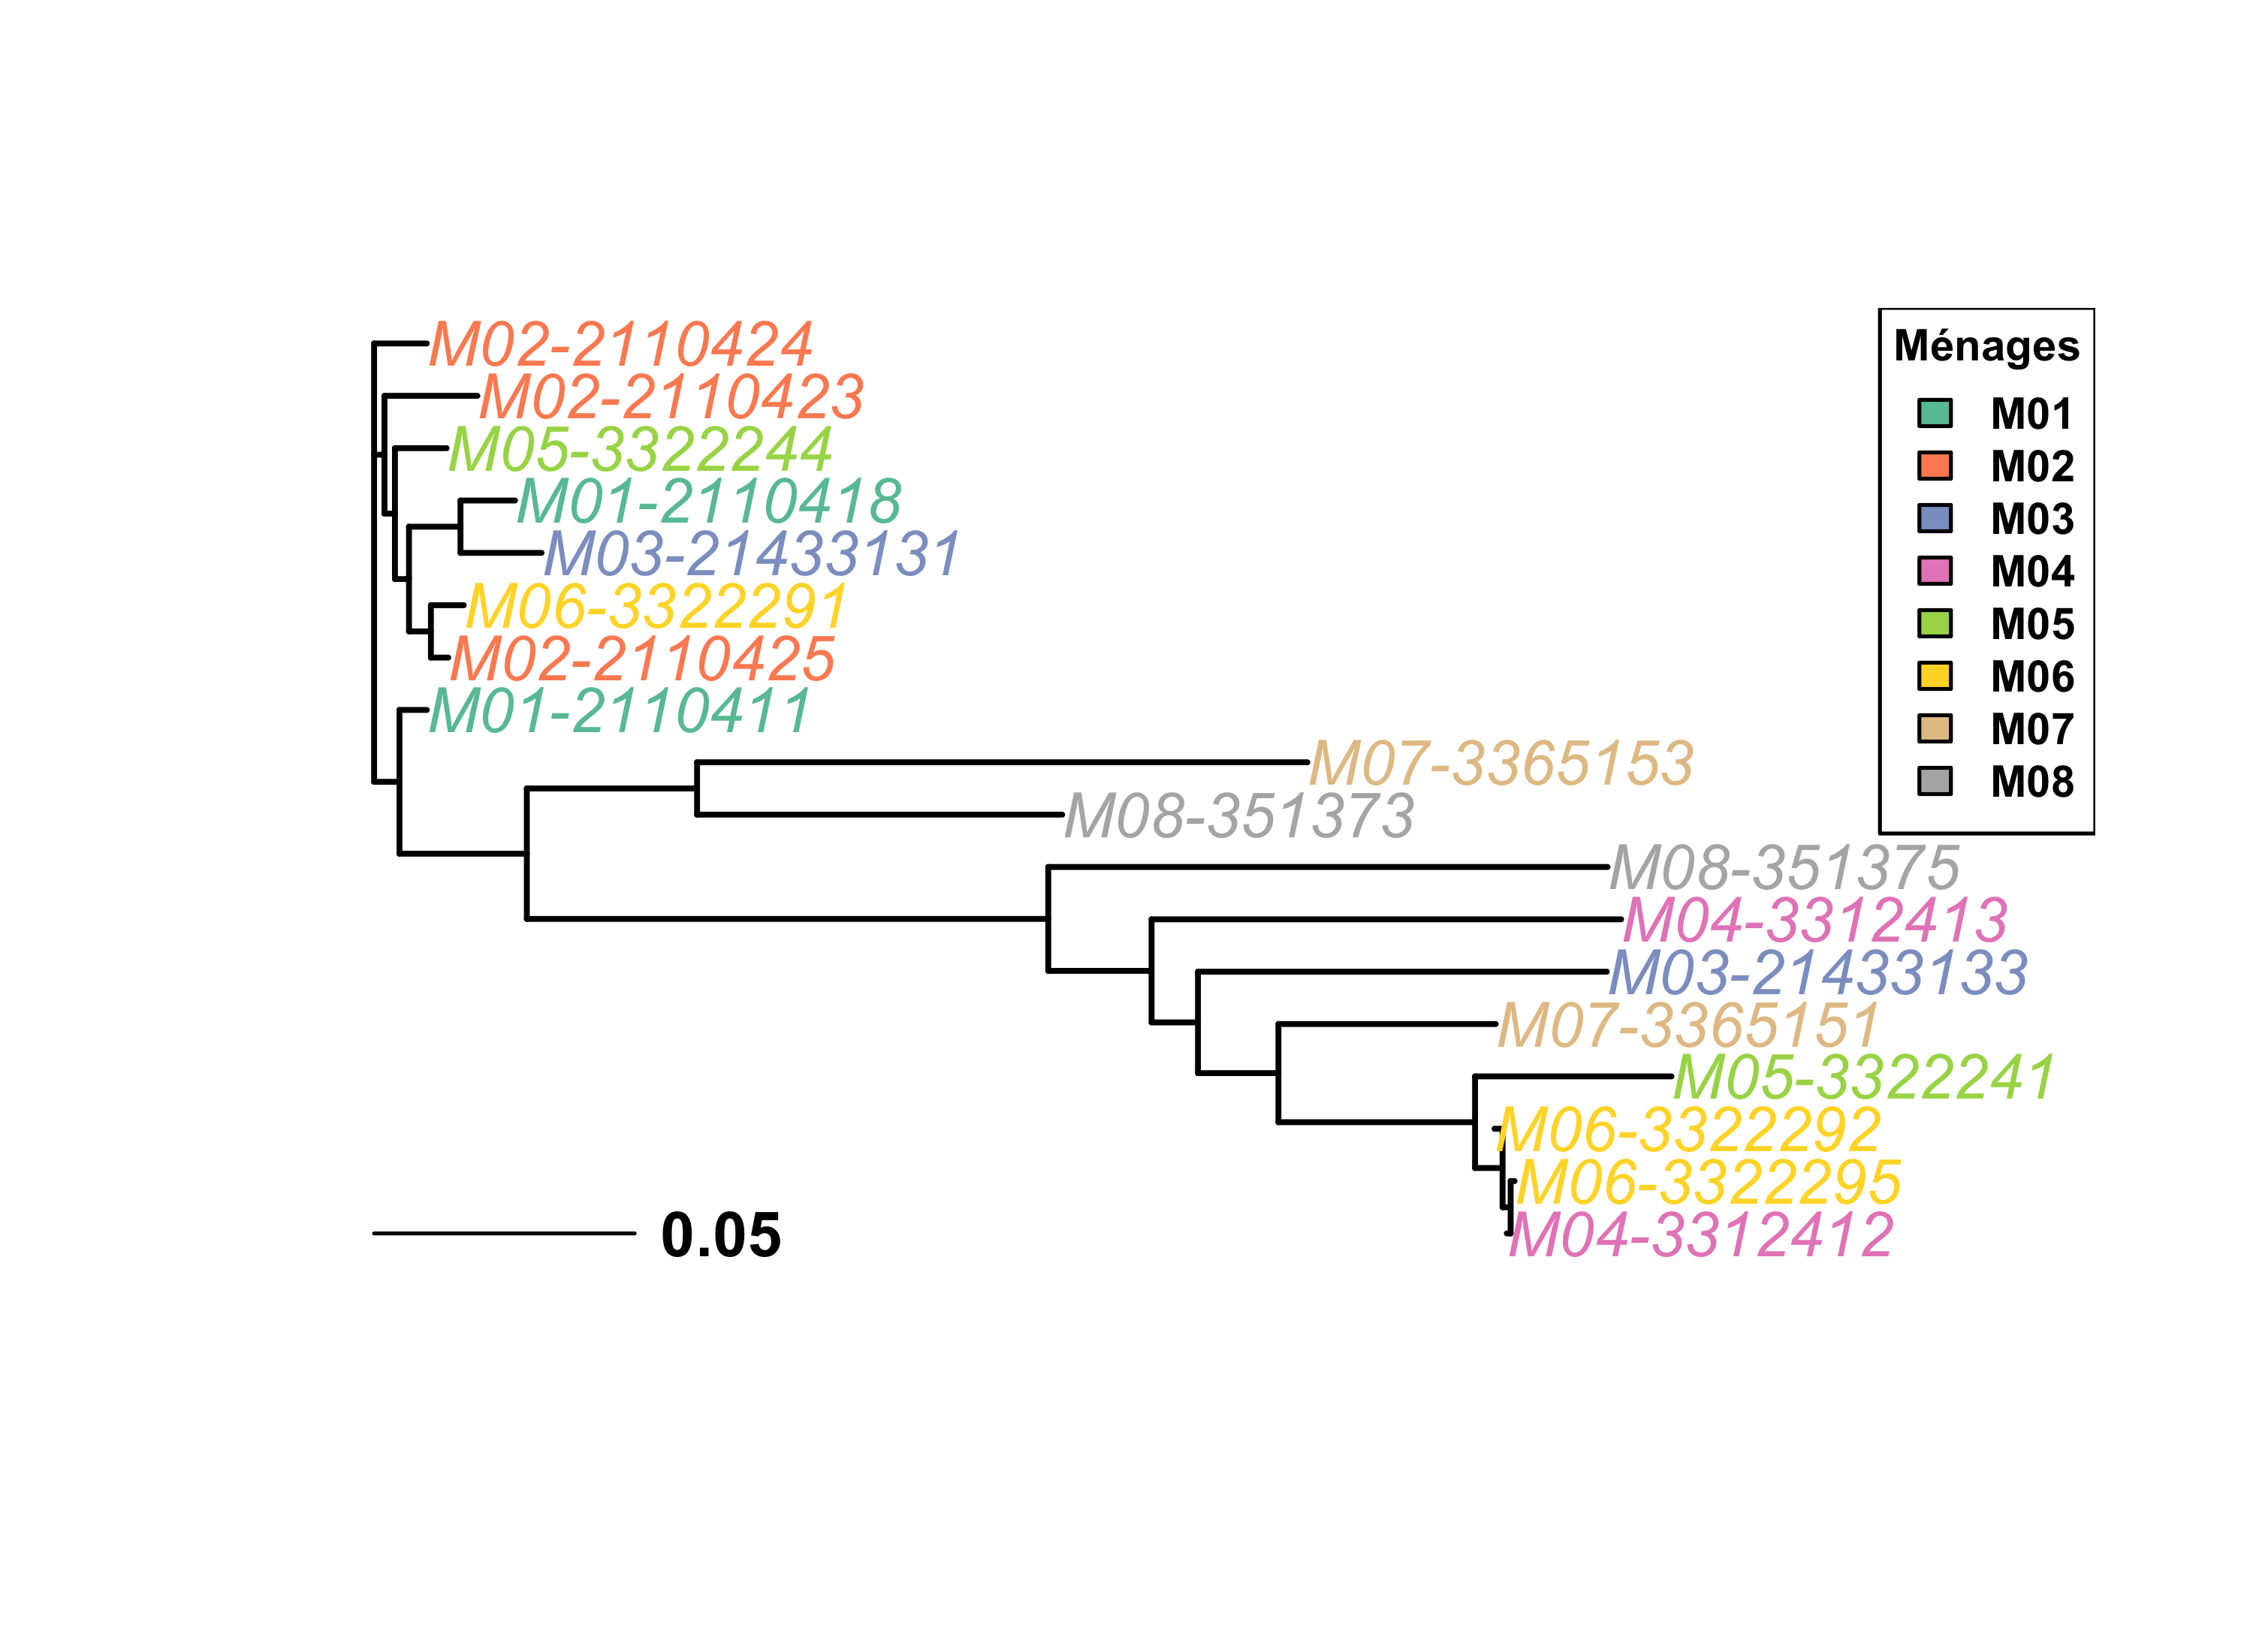
\includegraphics[width=1.18\linewidth]{./Image/phylogenie_VHCfoyerprimDist.png}
\caption{Phylogramme chez les foyer multiples: méthode distance}
 \label{fig:foyerM}
\end{figure}

\newpage
\begin{figure}[h]
\centering
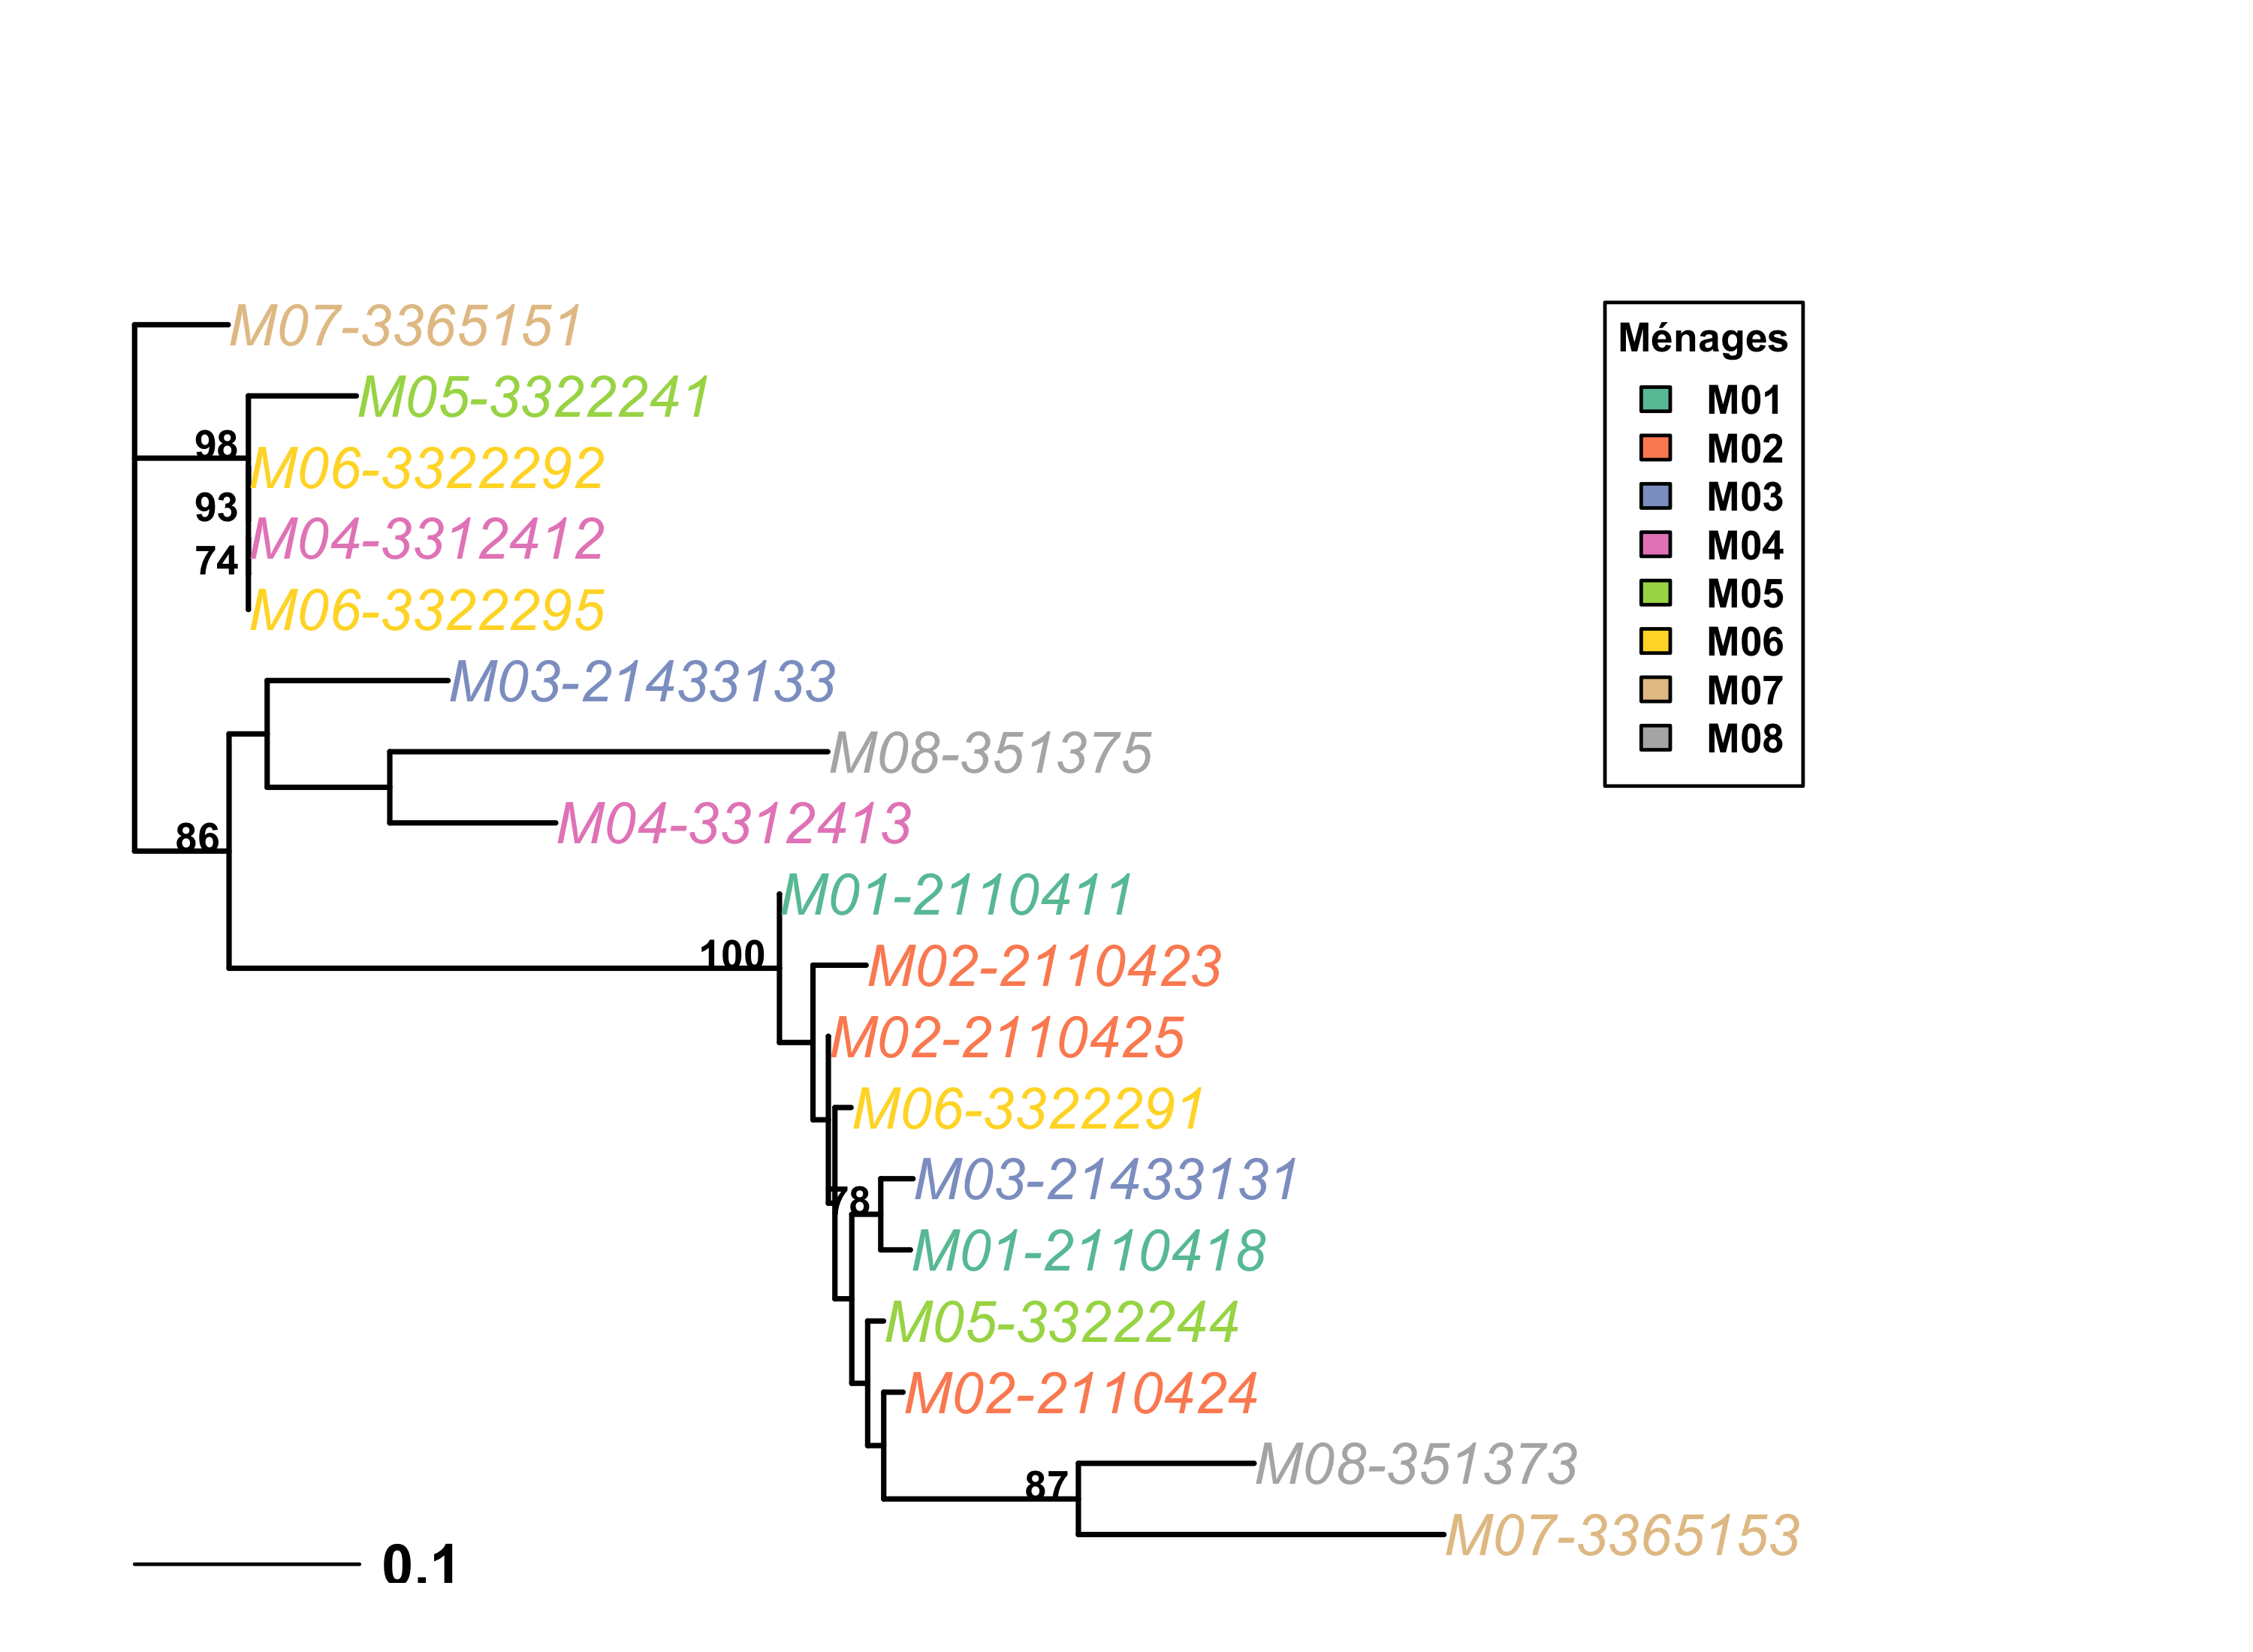
\includegraphics[width=1.2\linewidth]{./Image/phylogenie_VHCfoyerprimaryRAxml.png}
\caption{Phylogramme chez les foyer multiples: méthode ML}
\label{fig:foyerML}
\end{figure}

\subsection{Analyse phylogénétique : foyer multiple et groupe contrôle}

L’analyse phylogénétique intégrant les séquences des foyers multiples et du groupe contrôle en utilisant la méthode des distances (figure ~\ref{fig:Fcontrole}), montre que les séquences des foyers multiples ne forment pas un cluster totalement distinct du groupe contrôle. on constate toujours les sequences des individus ménages M04, M05 et M06 former un même clade, suggérant une proximité génétique compatible avec une circulation virale partagée au sein de  ménages (M06), tandis que d’autres sont plus dispersées et proches de séquences du groupe contrôle. 

Cette organisation indique une hétérogénéité des profils génétiques, ne permettant pas de conclure à une transmission intrafamiliale pour l’ensemble des foyers.

\newpage
\begin{figure}[h]
\centering
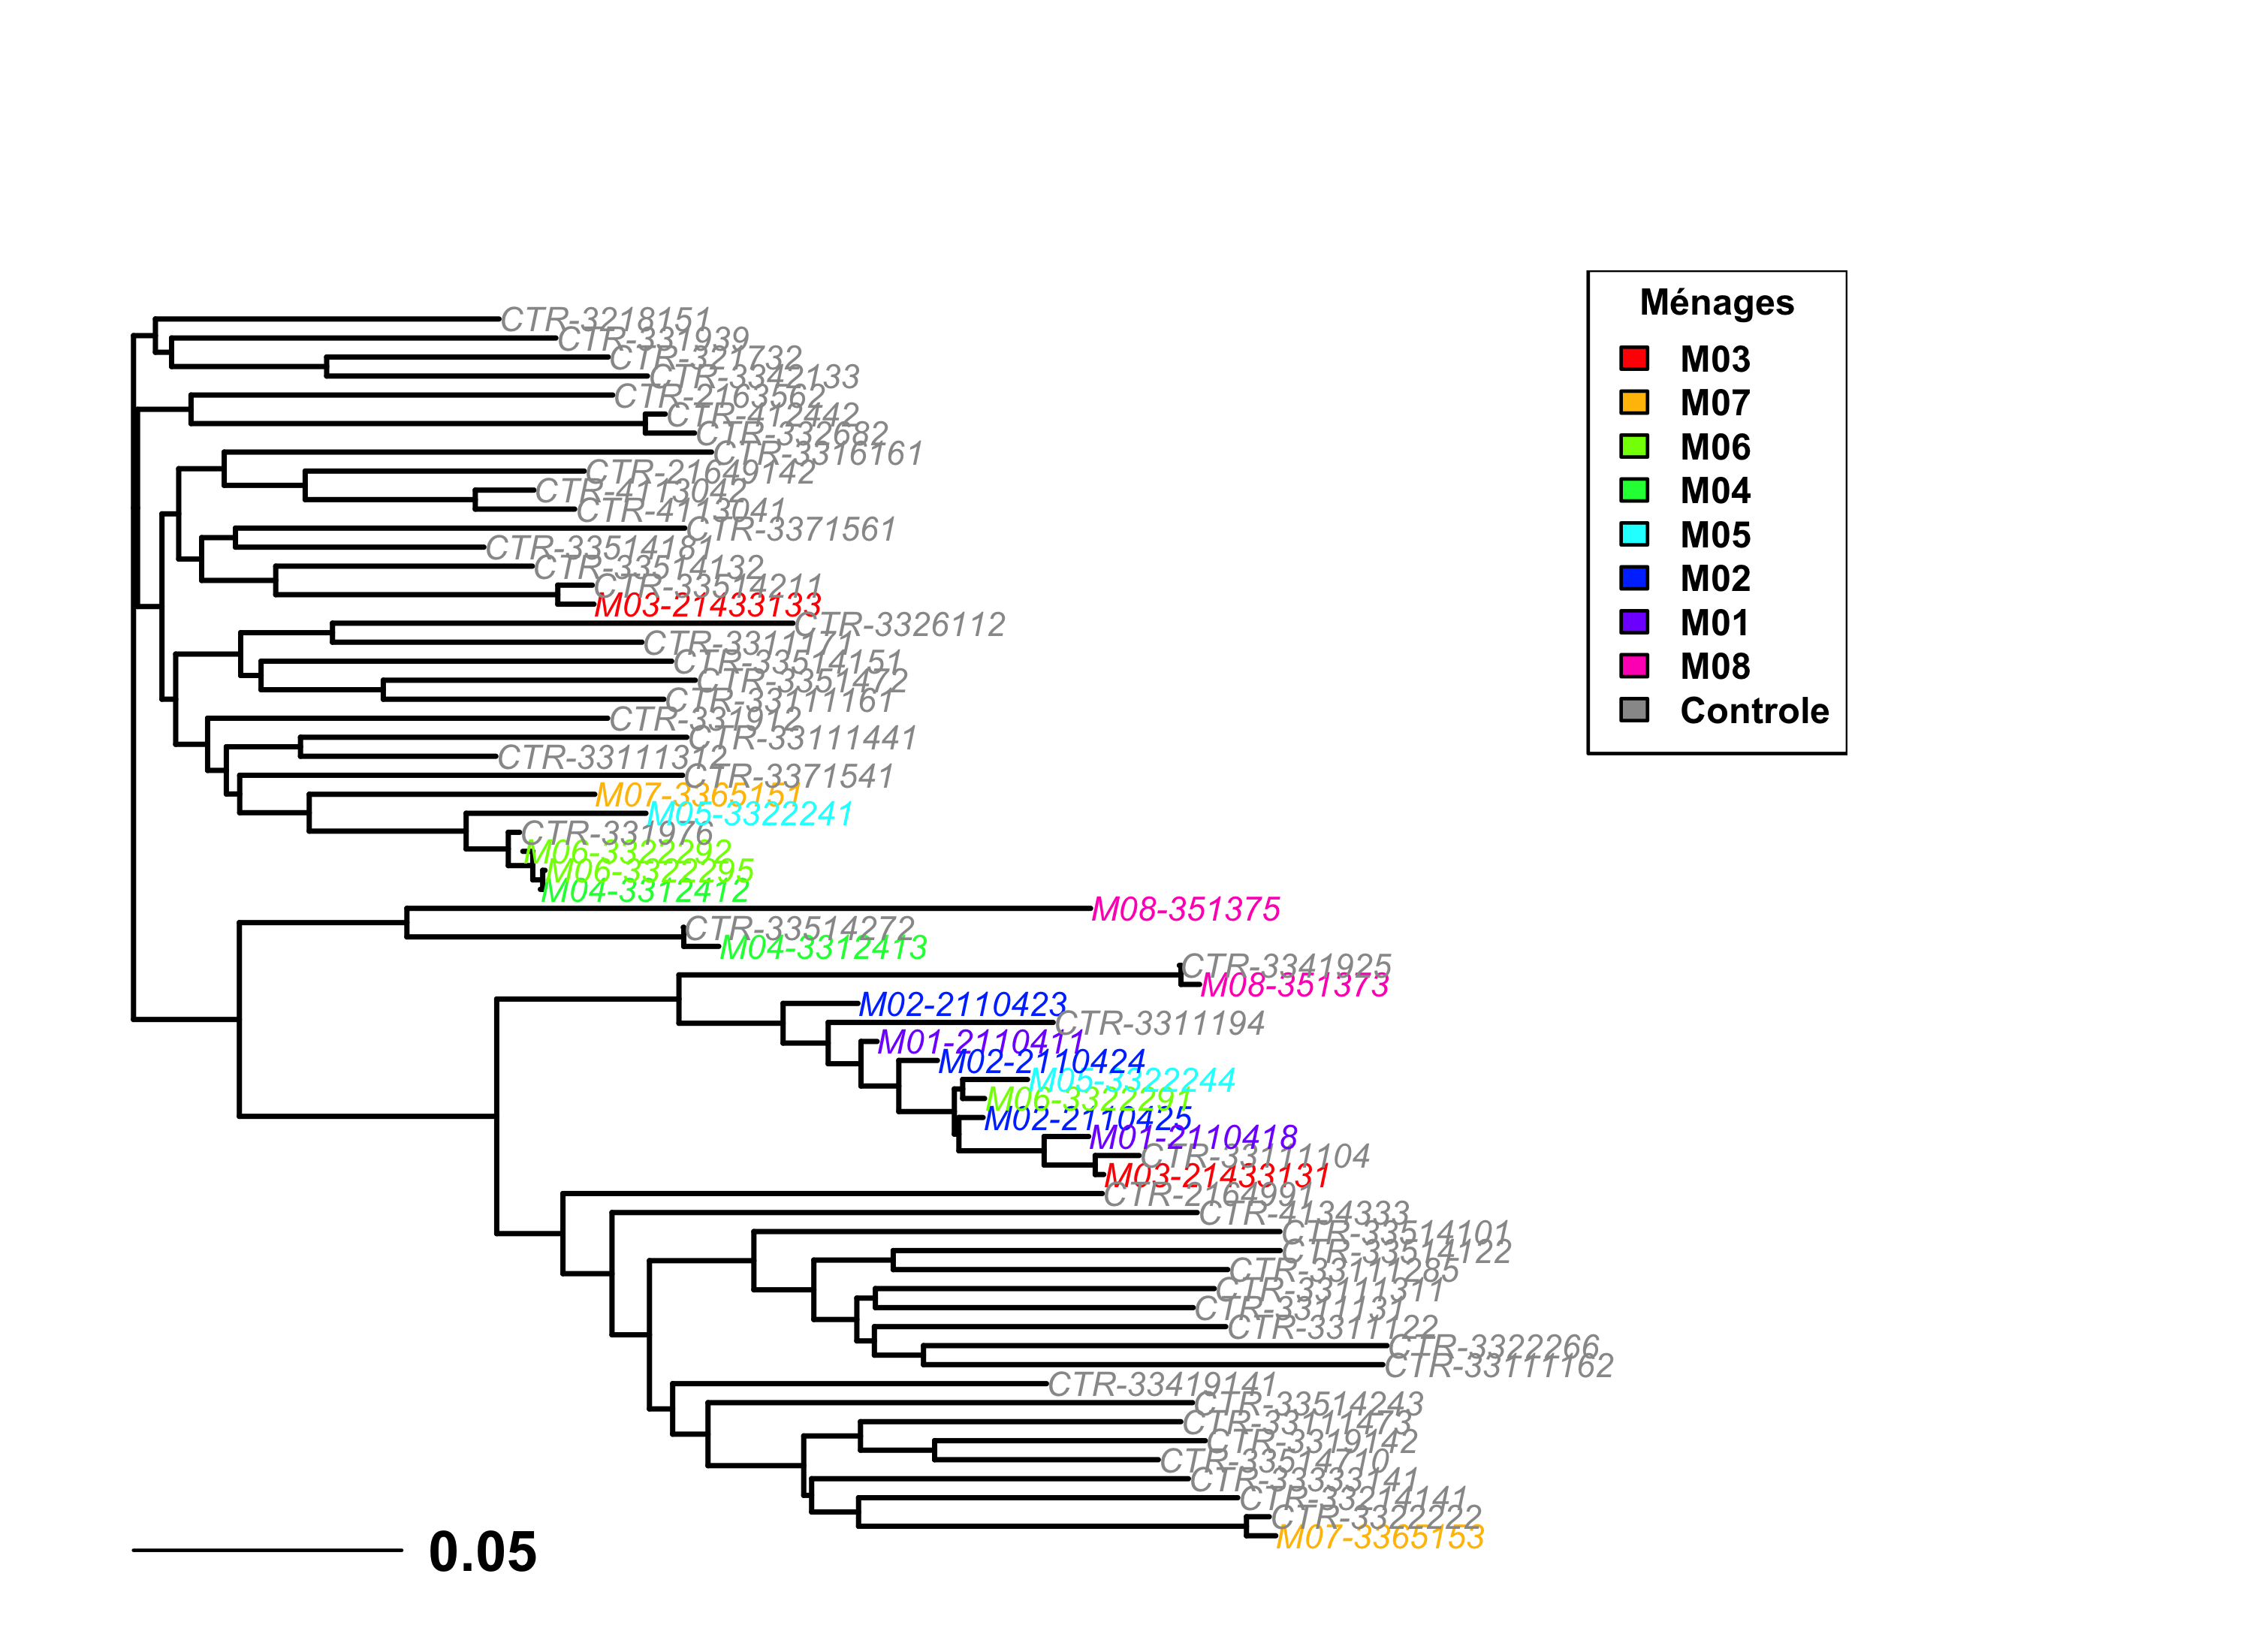
\includegraphics[width=1.18\linewidth]{./Image/phylogenie_foyer_controleDist.png}
\caption{Phylogramme des deux groupes: méthode distance}
\label{fig:Fcontrole}
\end{figure}

\newpage
\begin{figure}[h]
\centering
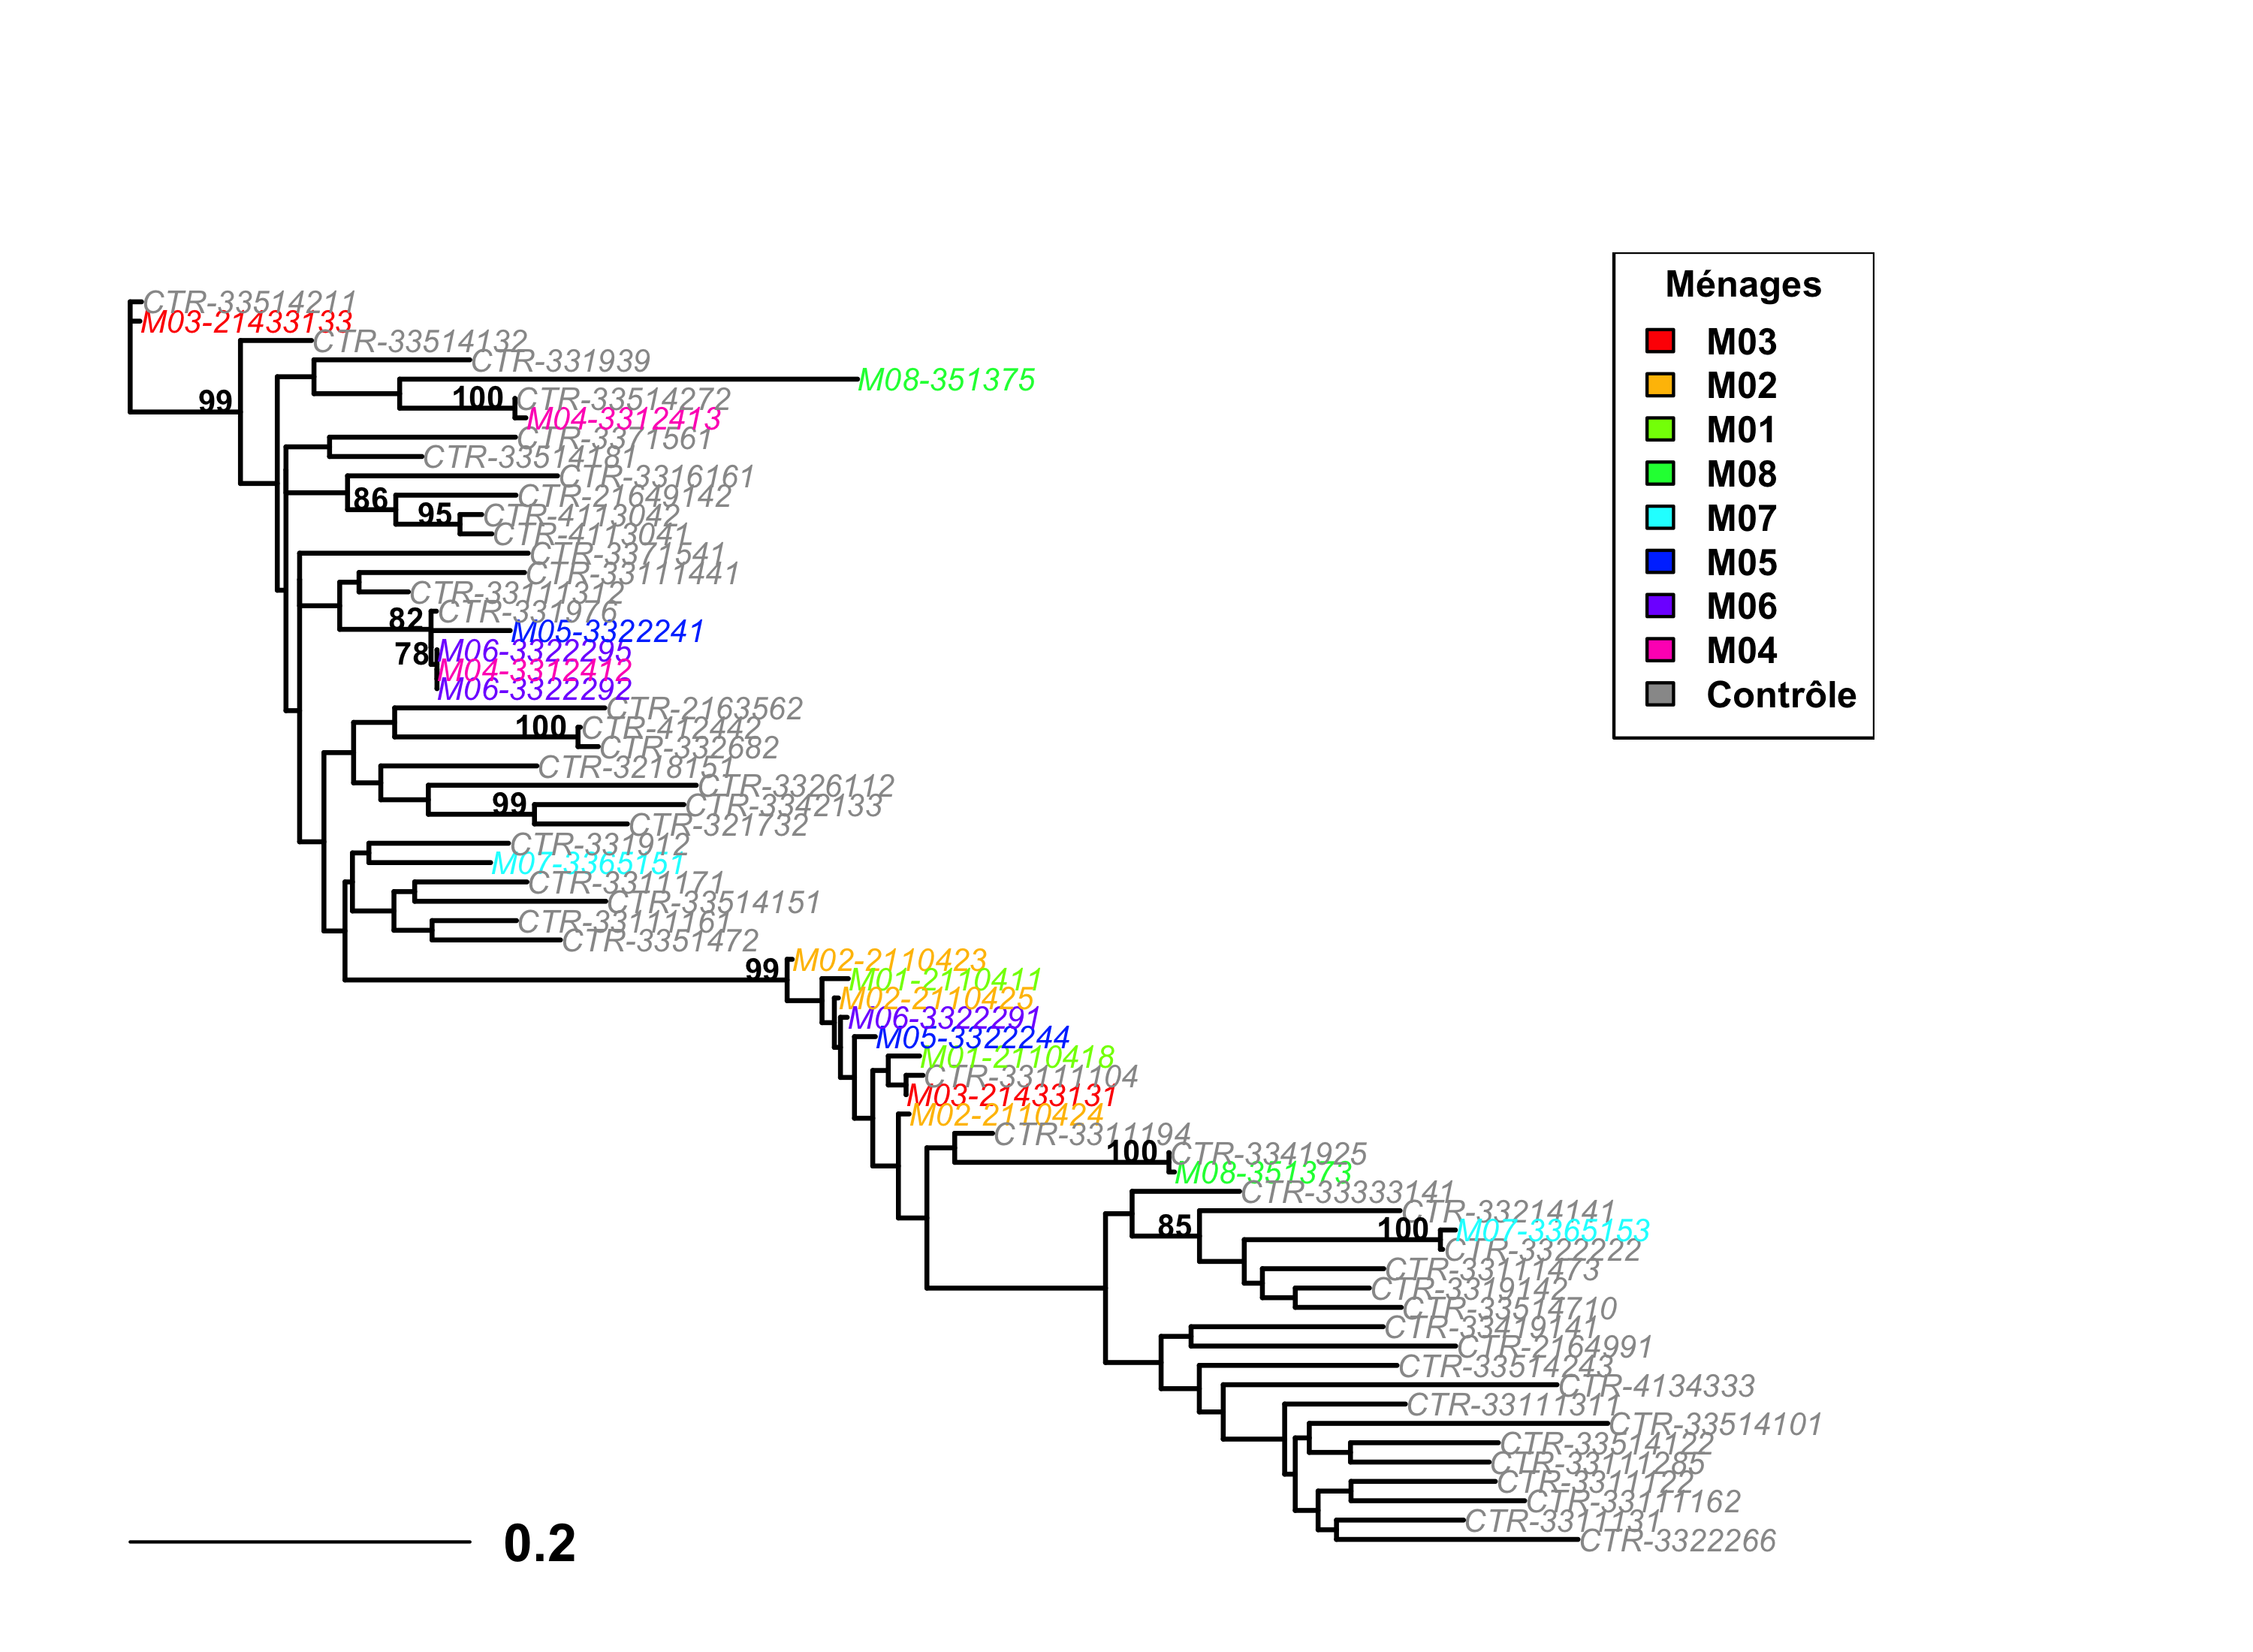
\includegraphics[width=1.18\linewidth]{./Image/phylogenie_VHCfoyercontroleRAxml.png}
\caption{ Phylogramme des deux groupes: méthode ML }
\label{fig:FcontroleML}
\end{figure}


\newpage 

\section*{CONCLUSION}
\addcontentsline{toc}{section}{CONCLUSION}

Globalement, l’arbre met en évidence des profils de clustering variables selon les foyers, traduisant des dynamiques de circulation virale hétérogènes, ce qui limite la conclusion d’une transmission pour l’ensemble des cas.

certains ménages montrent des regroupements robustes, compatibles avec une proximité génétique importante ;

la présence de bootstraps élevés appuie la solidité de certains clades ;

mais l’absence de clades monophylétiques stricts pour tous les ménages empêche de conclure à une transmission intrafamiliale pour l’ensemble des cas


\newpage 

\pagenumbering{Roman}
\setcounter{page}{4}

\printbibliography


\end {document}



